% Remove the oneside option below for double sided printing (e.g. for final (post-viva) submission)
\documentclass[a4paper,12pt,oneside,openright]{book}

% Preamble commands go here
\usepackage{customisations}

\usepackage{siunitx}
%% Some of the below packages may be useful to thesis writers in Physics
%% Googling `latex <packagename>' will usually give you some documentation
% \usepackage[load-configurations=abbreviations]{siunitx} % siunitx typesets physical units in a consistent manner
\usepackage{booktabs} % booktabs provides professional formatting commands for tables
\usepackage{amsmath} % amsmath provides extra maths symbols
\usepackage{textcomp} % textcomp provides extra text symbols (like a degrees celsius symbol)
% \usepackage{tikz} % tikz is a package for drawing diagrams and adding annotations to figures
% \usepackage{threeparttable} % threeparttable allows for adding notes to tables
% \usepackage{eps2pdf} % eps2pdf allows background transformation of eps files to pdfs so they 
%						work seamlessly with pdflatex. If using this with the LaTeX editor Kile,
%						you need to add --shell-escape before '%source', in
%						Settings -> Configure Kile... -> Tools -> Build -> build_pdflatex
\usepackage{mathtools} %To allow multiline eqns
\usepackage{blindtext}
\usepackage{pdfpages}
\usepackage{graphicx}


%Custom commands

\newcommand{\insertapproachfigures}[4]{
\newpage
\subsection{#2mM Site #3}
#4

\begin{figure}[ht!!!]
    \centering
    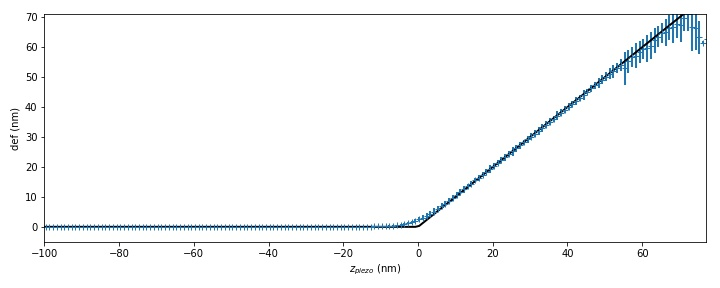
\includegraphics[width=0.7\linewidth]{chapter#1/#2/Site #3/approach_df_zp_bin}
    \caption{A graph demonstrating the binned average curve post fit for #2mM LiCl at contact site #3.}
    \label{fig:#2_site#3_forcezp}
\end{figure}

\begin{figure}[ht!!!]
    \centering
    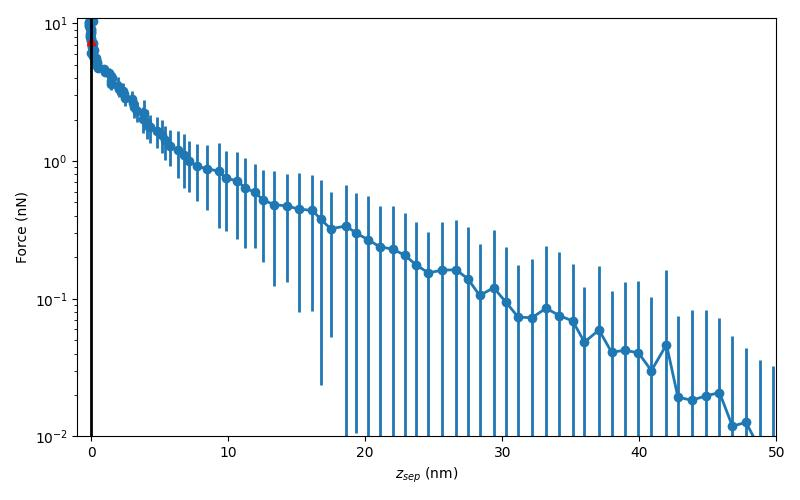
\includegraphics[width=0.6\linewidth]{chapter#1/#2/Site #3/approach_force_sep_log_lin_cont}
    \caption{A log-linear plot of the force as a function of the Z-piezo position, highlighting the interaction phase for #2mM LiCl at contact site #3.}
    \label{fig:#2_site#3_loglin}
\end{figure}

\begin{figure}[ht!!!!]
    \centering
    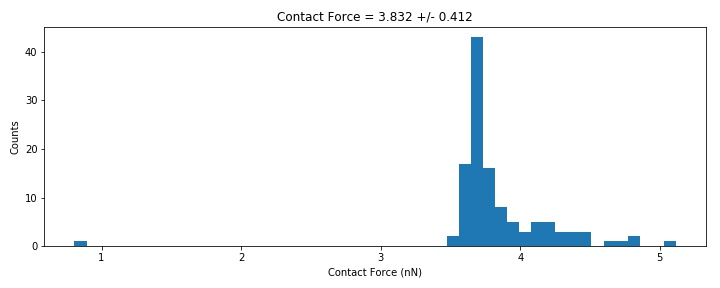
\includegraphics[width=0.7\linewidth]{chapter#1/#2/Site #3/approach_f_c_hist}
    \caption{A graph demonstrating the force histogram calculated from the range of curves for #2mM LiCl at contact site #3. The averaged contact force with the standard deviation is given above.}
    \label{fig:#2_site#3_hist}
\end{figure}
}


\newcommand{\insertsnowflakefigures}[4]{
\newpage
\subsection{#2mM Site #3}
#4

\begin{figure}[ht!!!]
    \centering
    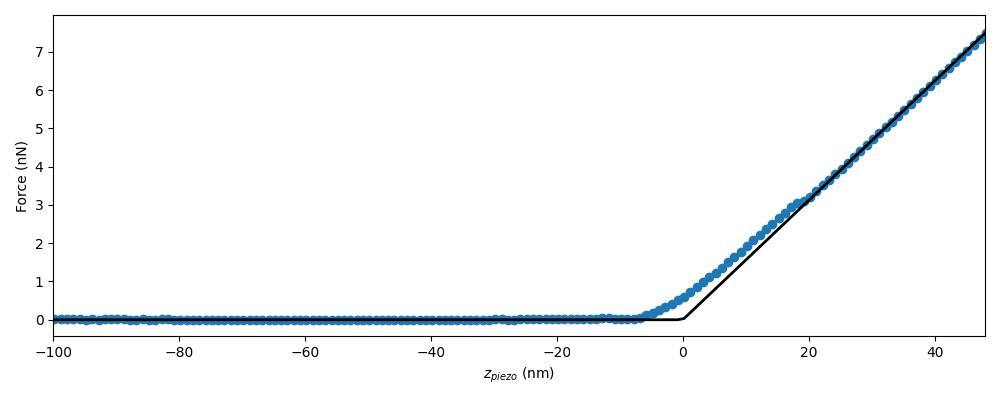
\includegraphics[width=0.7\linewidth]{chapter#1/#2/Site #3/approach_force_zp_bin}
    \caption{A graph demonstrating the binned average curve post fit for #2mM LiCl at contact site #3.}
    \label{fig:#2_site#3_forcezp}
\end{figure}

\begin{figure}[ht!!!]
    \centering
    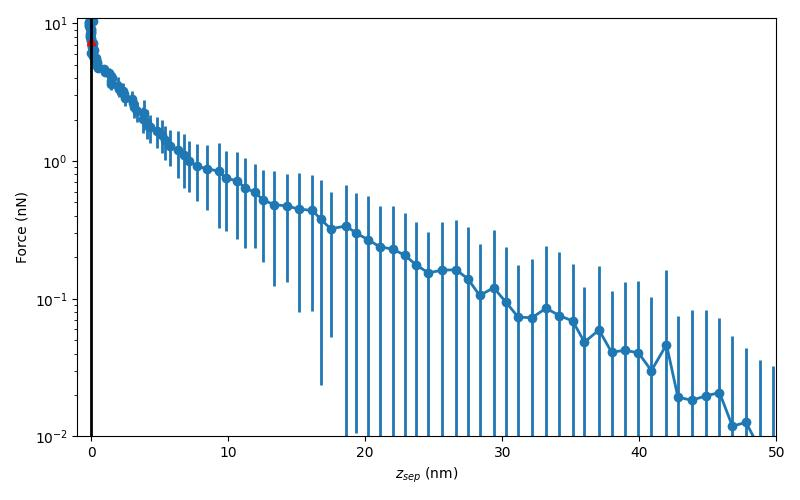
\includegraphics[width=0.6\linewidth]{chapter#1/#2/Site #3/approach_force_sep_log_lin_cont}
    \caption{A log-linear plot of the force as a function of the Z-piezo position, highlighting the interaction phase for #2mM LiCl at contact site #3.}
    \label{fig:#2_site#3_loglin}
\end{figure}

\begin{figure}[ht!!!!]
    \centering
    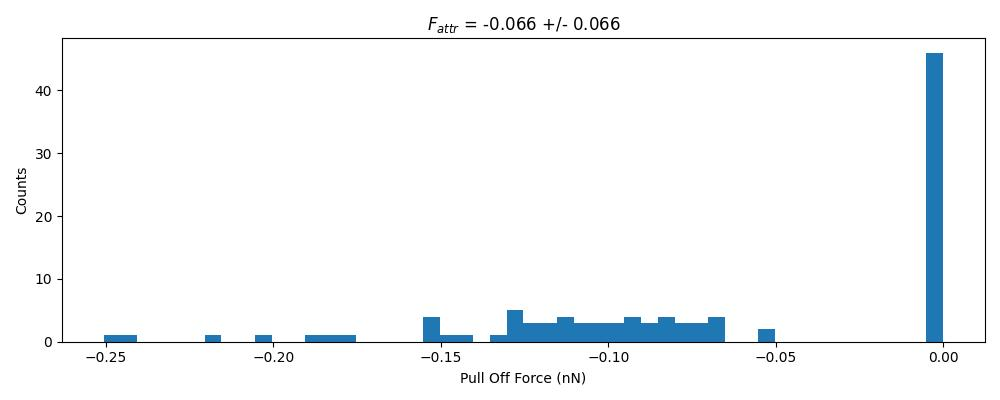
\includegraphics[width=0.7\linewidth]{chapter#1/#2/Site #3/approach_f_a_hist}
    \caption{A graph demonstrating the force histogram calculated from the range of curves for #2mM LiCl at contact site #3. The averaged attractive force with the standard deviation is given above.}
    \label{fig:#2_site#3_hist}
\end{figure}
}

\newcommand{\insertretractfigures}[4]{
\newpage
\subsection{#2mM Site #3}
#4

\begin{figure}[ht!!!]
    \centering
    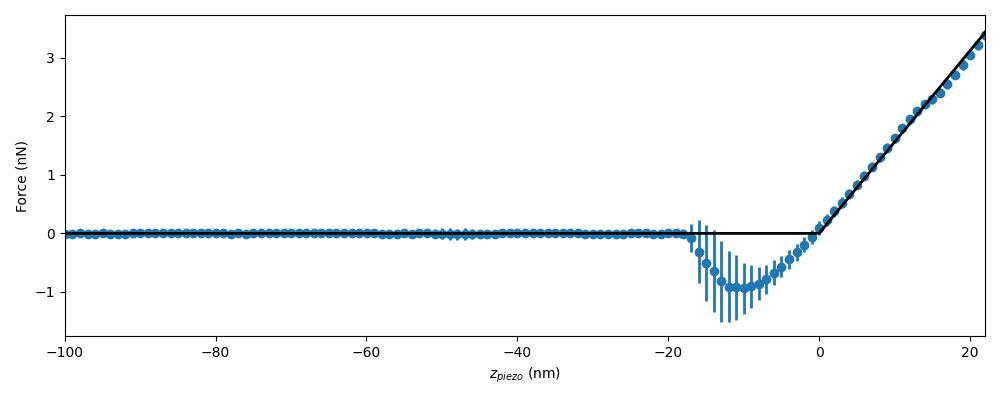
\includegraphics[width=0.7\linewidth]{chapter#1/#2/Site #3/retract_force_zp_bin}
    \caption{A graph demonstrating the binned average curve post fit for #2mM LiCl at contact site #3.}
    \label{fig:#2_site#3_forcezp}
\end{figure}

\begin{figure}[ht!!!]
    \centering
    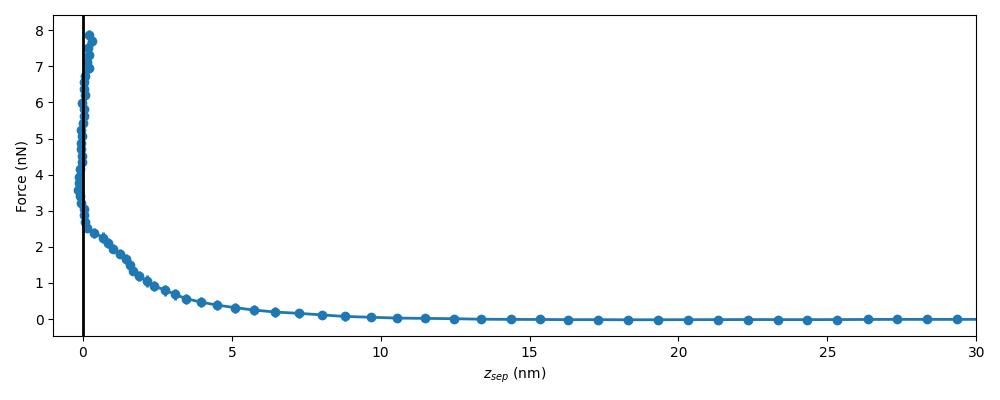
\includegraphics[width=0.6\linewidth]{chapter#1/#2/Site #3/retract_force_sep}
    \caption{A linear plot of the force as a function of the Z-piezo position, highlighting the contact phase alignment for #2mM LiCl at contact site #3.}
    \label{fig:#2_site#3_loglin}
\end{figure}

\begin{figure}[ht!!!!]
    \centering
    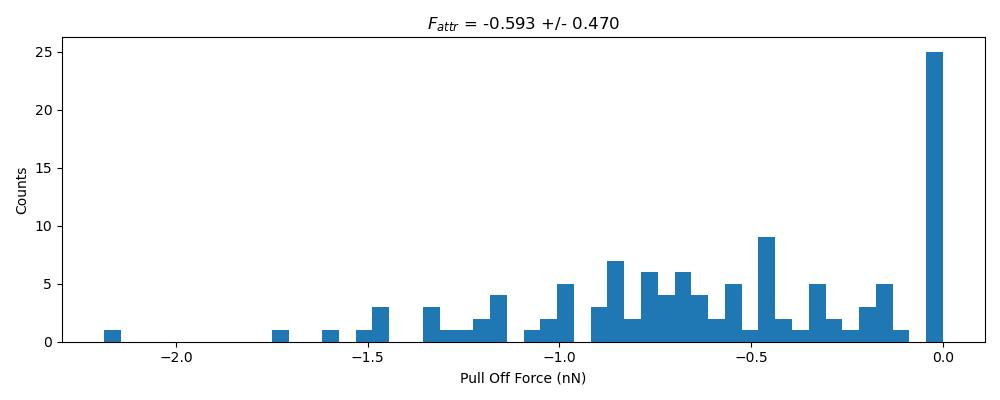
\includegraphics[width=0.7\linewidth]{chapter#1/#2/Site #3/retract_f_a_hist}
    \caption{A graph demonstrating the force histogram calculated from the range of curves for #2mM Li




% End preamble

% REPLACE THESE with your thesis title, your name and the date of submission of the thesis


\begin{document}

%Regulation 34
%\section{Regulation 34 agreement}

Regulation 34: “Every student must incorporate a signed declaration in the thesis, research project or dissertation submitted for assessment, stating:

(a) That the thesis, research project or dissertation has been composed by the student, and
(b) either that the work is the student’s own, or, if the student has been a member of a research group, that the student has made a substantial contribution to the work, such contribution being clearly indicated, or
(c) that the work has not been submitted for any other degree or professional qualification except as specified, and
(d) that any included publications are the student’s own work, except where indicated throughout the thesis and summarised and clearly identified on the declarations page of the thesis.”

Signed:

$Joseph$ $French$

\tableofcontents
%Background
%Reviewing/done
%\chapter{Introduction to surface forces}
%Intro
%Surface forces - van der waals, electrostatics, charge screening, DLVO, derjaguin
%hydrodynamics - lubriciating, viscous forces
%brownian 
%Rheology - bulk & translation, shear thickening, friction, industry
%MOVE OUR SYSTEM TO CHAPT4
%Conclision
%Check what I define what a long range force is, what is a short range force is?
%add nomenclature/glossary
%Where is Ue(r) defined ?
%REFERENCES ARE BUGGERED PLEASE FIX BEFORE SENDING OFF TO BE READ!!!
 
\title{Introduction}
%The methods of how particles interact with one another has been a longstanding area of interest in physics. As matter encroaches upon one another %there in an interplay of attractive and repulsive forces.
The fundamental interactions between particles has long been an area of active research in physics. The interplay of attractive and repulsive forces which occurs at the boundary between particles is both difficult to understand and vital to master.
%These forces and mechanisms are known as interacting surface forces, and the interplay of these interactions define the systems we experience and observe in day to day life. Some examples include the wetting of surfaces from an interfacing liquid or the means in which an organism adheres to a surface. 
Examples of the emergent behaviour which arises from these interactions includes the spreading of a water droplet across a surface and the adherance of micro-organisms to surfaces.
These forces
%while from the perspective of the universe are nothing new,
have
%gained
recieved increasing interest and understanding over the last century
%to
from scientists and industry alike. The demand for a clear and concise picture of these interactions only increases as innovations in technology rely more and more on these interactions, from touch screen developments, 
%water resistant
superhydrophobic surfaces, bacterial frustrating surfaces or even the humble custard. 
There are several ways to 
%flirt with
probe these forces 
%either as an innovator; 
either by chemically treating the surface, altering the physical structure of said surface or by altering the
%inter-facial 
nature of the 
%solute 
solution said surface finds itself involved with. By changing these properties, new promising technologies can 
%push
advance our understanding of such 
%a
systems.
%to it's limits. 
As %scientific study
researchers become
%s
more and more involved on 
%elucidating
studying these interactions,
%on the molecular scale
 we find more and more of the world we live in is 
%defined by our understanding 
a result of the emergent behaviour of such systems and as a result, it is imperative to not only question the history of our combined understanding, but to test such systems experimentally.
%The history of surface forces finds itself
Our modern understanding of surface forces is derived from van der Waals 
%forces, 
theory,
%a theory produced by 
the result of a series of papers produced by London, Debye and Keesom \cite{AFMvdW}. %These 
Attractive forces were combined with repulsive double layer forces to %form 
give the main theoretical basis %of 
for particle-particle interactions, %consequently 
subsequently %known 
referred to as DLVO theory (derived from Boris Derjaguin and Lev Landau, Evert Verwey and Theodoor Overbeek) as a result of two groups reaching the same conclusion independently\cite{Verwey}\cite{DERJAGUIN}. This underlying theory describes the %resultant 
surface forces felt between two particles in solution .
%From these simple particle-particle interactions bulk behaviours are derived, 
More complex behaviours arise emerge as a result of these interactions - for example %such as the case for 
colloidal systems. Mixed phase suspensions, called colloids are a combination of a solvent and a solute. Indeed, one only has to look inwards to find a fascinating colloidal system (albeit a very complicated one). \cite{surfThesis} \cite{christian2018a}
Systems defined by inter-molecular forces are prevalent in a wide range of applications, said theory providing the basis for several industries such as water purification, batch processing (food, pharmaceuticals, detergents, paints) and mining.\cite{TABOR19772}
%Born from (history)
\section{Forces between molecules}
%wrong - don't trust interpretation 
Inter-molecular forces are essentially electrostatic in nature, as postulated from quantum theory, initially defined by the Hellman-Feynman theorem. %From the Coulomb force and complex fluctuating forces observed around the surfaces of atoms. 
However, %simple solutions to the Schrödinger are hard to come by, 
solving Schrodinger's equation for poly-atomic systems is very difficult and as such, this unified force is fractured down into smaller %classifications 
components to simplify their definition and %equation
computation. These categories are %known as 
ionic forces, van der Waals forces, hydrophobic forces, hydrogen bonding and solvation forces. 
%Covalent / coloumb interactions, short range and strong
Chemical bonding depends on the interaction of neighboring atomic orbitals, while steric forces arise from quantum mechanical or electrostatic interactions between separated particles. %They are an emergent property of the electronic structure of the atoms, as apposed to a molecular orbitals, where the molecular configuration is in a state of semi-perminance and free from flux changes.
%A main difference between the two is the permanence of charge distribution changes, where in the case of the former is retained as long as the bond is retained.
Coulomb's %forces 
law %are 
describes the force %of the charge effects of two charges applied upon one another with respect to distance. 
which arises from the electrostatic interaction of charged particles:
%loose
%In  approximation the inverse square force is given by: %Not atoms per say
%Why is this the simpliest
\begin{equation}
F \propto \frac{Q_1 Q_2}{kr^2}
\end{equation}
Where upon this can be expanded into:
\begin{equation} %\frac{Q_1 Q_2}{4\pi\varepsilon_0\varepsilon r^2} =
F = -\frac{dw(r)}{dr} =  \frac{z_1z_2e^2}{4\pi\varepsilon_0\varepsilon r^2}
\end{equation}
where w(r) is the free energy of the Coulomb interaction, r is the distance between the two charges Q\textsubscript{1} and Q\textsubscript{2}. $\varepsilon$ is dielectric constant of the medium, and z is the ionic valency of the atom in question, in relation to the elementary charge e. % Due to it's inverse square law nature it is a force highly dependant on distance. 
The inverse square relationship between the free energy of interaction and distance between the point charges makes this force drop off sharply as the distance increases.
%w(r) is Joules, ~ 8x10^-19J, kT is 5x10^-21J. Stronk.
%lennard jones potential here?
\section{Brownian Motion}
%Traditionally; 
The term colloid was coined in 1861, drawn from the Greek word $κόλλα$ (kolla), meaning glue, from Thomas Graham's observations of particle aggregation\cite{old_colloid}. %Nowadays 
today, a colloid is defined as %the intermixing 
a mixture of two separate phases; a dispersed, suspended phase and a continuous%, medium
phases in which the former find themselves in. %For our area of interest, we place our scope on a particular colloidal suspension; a dispersion of solid particles within a liquid medium. 
Colloids consisting of solid particles suspended in a liquid medium shall be the focus of this thesis.\cite{review_colloid1}
Consider the idea of marbles kept within a liquid. At rest, they would lie upon the bottom of the container, yielding to the force of gravity\cite{Neuton}. However, as you scale down these marbles, to smaller and smaller sizes, the kinetic energy of the system is enough for keep the marbles dispersed within the liquid, due to Brownian motion\cite{Brown}.
At micrometer sizes however, the marbles begin to affect one another; when two marbles are brought together by Brownian motion, provided the interactions between the two of them are attractive, they will attract towards each other, and eventually aggregate, until they are large enough to sediment again. If there is no attraction, or indeed repulsion, between the marbles, they will stay suspended within the solution.
%Interactions between the marble's surfaces, are defined by a few fundamental forces resolving linearly with one another. These interplay of forces, borne from electrostatics, van der Waals and solvation forces, all sum up into a force profile based on distance between the two surfaces.
The various interactions between the marble surfaces can be combined to give a force profile, describing the strength of the interaction between the marbles with respect to the distance between them.
These force profiles depend upon a number of % intrinsic 
properties intrinsic to the phenomena. %To define these variables in a broad stroke; the liquid the solid colloid is immersed in (liquid phase properties), the surface properties of the solid phase (solid phase properties) and interactions between same phase particles (same phase interacting properties).
On the macro scale, these interactions %equal out to resolve into their 
ultimatley contribute to bulk properties. As this system is disturbed by external forces, a 
%resultant 
characteristic relaxation time is observed, dependant on the ions in solution and surface properties of the solid phase particles. %From these disturbances, new dipole moments can arise additionally. 
These properties give rise to the %hysteric effects 
time dependent effects seen in systems such as these.
With such a complex system of non trivial interactions, the history of elucidating such a complex system has not been a simple one. Ideally in physics finding a unifying, complete equation to describe all manner of interactions would be the goal, however, even if that were possible, colloidal systems are not frozen in an equilibrated state and are the result of combining relations between intrinsic properties and dynamic, sympathetic effects. As such the current state of the theory relies upon simplified simulations to push forward the field, and as such, an experimental analysis %upon 
 of said models is required. \cite{FoundColloidBook}\cite{IsGreenBook}



%AFM background
% Should be done??
%\chapter{Atomic force microscopy}

%Todo
%Anatomy of a force curve with chapt 4-6 in mind
%Force mapping
%uhhh
%Tip speed 
%Hydrodynamic effect on tip (specifically on tip, hydrodynamic forces in chapt 1)

\section{Introduction}
The origins of microscopy are believed to date back to the thirteenth century, stemming from the development of eyeglasses and spectacles. The first practical microscope, which utilized the visible spectrum to image samples through photonic light, evolved over centuries into what is known today as the light optical microscope. However as the optical microscopy design improved, it eventually hit a major limitation - the diffraction limit of photons. New techniques and designs were created using methods to overcome this limitation, circumventing the limitations of photons. These novel methods expanded the scope of microscopy beyond its initial reliance on emissions from the visible spectrum. Some such examples include phase contrast microscopy, electron microscopy and local probe microscopy. While these techniques share a name and history, there are major practical differences between them.

Local probe microscopy particularly differentiates itself from other microscopy techniques as it does not rely on a trans-migratory radiation particular source to convey information on the exposed sample. Instead, an image is generated by physically probing the surface with a specialized tip, wherein the tip's physical location becomes the key means of conveying information about the sample. This is in contrast to various microscopy techniques, which generally use some form of radiation to interact with a sample. The differences between these two results in different data structures for each respective technique. \cite{giesbers2001surface}
%Above might be a bit janky - poor flow?

The first progenitor of the probing microscopy family, the Scanning Tunneling Microscope (STM), was invented in 1981. This pioneering technique allows for mapping the topography of a conductive surface with atomic resolution. In STM, the probe's height above the surface is determined by the tunneling current that flows when the conductive tip is brought within approximately 1 nm of the sample. This current occurs due to quantum tunneling, where electrons pass from the tip to the surface (or vice versa) depending on the bias voltage applied. The tunneling current is highly sensitive to the distance between the tip and the surface, decreasing exponentially with increasing distance. By maintaining a constant current (which implies a constant tip-surface separation), the STM can map out the surface topography with remarkable precision.\cite{STMreference}
%Missing citation (add to bibtex)

Atomic force microscopy (AFM) is based on the force between the tip and the sample and tracks the physical location of the probe tip via a reflected laser. This enables the analysis of both non-conducting samples and samples that needs to be in liquids. It is this versatility and adaptability that AFM allows that gives it one of it's greatest strengths. The method is novel compared to conventional microscopy techniques as it does not rely on lenses for observation; instead the position of the stylus is detected by a laser reflecting off the surface of the cantilever. Equally, issues of absorbance or transparency are negated, as the results are of a physical contact nature. By probing the surface of a specimen the surface characteristics can be observed, such as the hardness or elasticity of a sample, all while remaining a relatively non-destructive method of imaging. AFM can be specialised further with specific tips or attaching specific molecules to detect surface chemistry, adhesion or arrangement of ions on a surface\cite{KislonAfm}. 

%The tip itself is comprised of a nanometer sharp stylus mounted on a flexible cantilever. Upon the back of cantilever is a reflective surface; some common examples being antimony and gold, which is used to reflect the detecting laser back. This probe is mechanically driven over the surface using a piezoelectric motor where the sharpest point of the stylus grazes atop the surface of a sample returning height data as it moves. As the probe interacts with the surface the cantilever bends in response to the surface below, with the piezo motor adjusting the pressure applied to the sample based off the deviation of the reflected laser angle. As this setup bends, so too does the reflected laser angle shift, with the motor automatically compensating and moving in response to this. It is from this movement that the recorded height is calculated.

As a result of these phenomena, AFM stands out when compared to light microscopy. Its intrinsic ability to resolve images at nanometer length scales, overcoming the optical diffraction limit of standard microscopy techniques, means that it is one of the best methods to view and interact with samples non destructively. Since AFM's resolving power is limited by the radius of the tip, different tips can be used depending on the application such as nanometer sharp tips to resolve on the atomic scale, tips with a specialised surface chemistry or tips for use in liquid conditions. A further strength is the ability to image specimens under different conditions; within air, water, or especially in the case of biological samples; within buffers to reduce the adverse effects of observing samples. \cite{WetAFM}. 

Another benefit that AFM provides to its operator is the ability to measure small forces acting between the tip and the probed surface. This interaction is particularly useful in measuring single particle interactions, and is one of the major methods used in this thesis described below.

%This is observed by the small attractive or repulsive forces bending or pulling the cantilever towards or away. This interaction is measured over distance from approach or retract, giving a detailed surface force profile at different separation distances.

With all these benefits there comes a cost. There is a large amount of interplay between each of the different forces, geometries and mechanisms; meaning that interpretation of recorded data is usually more complicated compared to an image produced by light microscopy. As a result, there is an art to AFM that every operator has to learn and master in order to gain meaningful data. Futhermore, it is on the operator to prove that their interpretation is accurate and avoid some of the common pitfalls in using the technique.

\section{Basic overview of AFM operation}

In order to describe in detail the methods used in this thesis for data collection, a basic understanding of how AFMs work must be understood. While some AFMs differ in design and implementation, they all rely on largely the same fundamental design and principles. 

All local probe microscopes rely on the same mechanism, the information gathered from a sample comes from an interacting probe. Consider the example of a blindfolded person using a cane to map out the surface in front of them: the map they put together in their mind would represent the topology of the space around them. AFM works in largely the same way, but in place of a mind is a computer, and the cane itself is a much smaller cantilever. Instead of the surface being felt out by hand it instead uses a few sensors to determine the sample's properties. While the range of output variables is relatively small compared to other methods, these can be greatly expanded upon by transforming this information to give properties such as elasticity, attractive and repulsive forces and more. This interaction is then processed across the sample window, giving a map of different information with respect to lateral position.

\begin{figure}[h]     %Insert a figure as soon as possible
        \begin{center}
          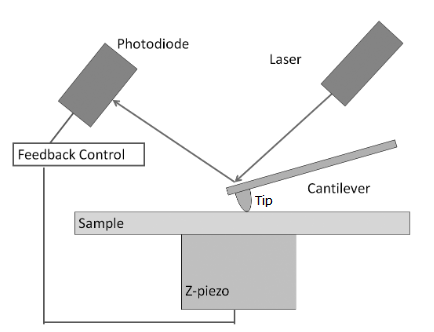
\includegraphics[width=110mm]{chapter2/RAFMSch.png}
\end{center}
\caption{A basic schematic of an set up AFM. Image adapted from \cite{RAFMSchRef}.}
\label{fig:AFMSch}                 % Reference label to the figure.
\end{figure}


%use "origin" rather than "0,0"
The general schematic of an AFM is shown above (figure \ref{fig:AFMSch}). The only directly interacting point upon the sample is the tip (which is mounted on a cantilever), keeping the interaction between the sample and mechanism to a minimum. A laser is emitted and aligned to the head of the cantilever above the tip. This laser is then reflected off the back side of the cantilever into a photodiode which converts input light into an output electrical signal. Initially the laser is set up to reflect into the origin position (the center) of the photo diode. This ensures that it has the maximum amount of room to translate across the surface as the cantilever deflects. As the tip is brought into contact with the surface the cantilever bends and relaxes as it processes over the sample. These translations alter the reflected angle off the cantilever, depending on the underlying sample surface topography. This reflected light then changes the positioning of the detected light on the photodiode, translating its x, y component relative to the alterations of the cantilever. The cantilever itself is moved across the surface by a piezoelectric motor with a high degree of precision. In some implementations, the piezo is singularly used to control the height position (z axis) of either the stage, or the tip. However, particularly in imaging mode AFMs, the piezo can additionally accommodate lateral and horizontal (x and y axes) movement. Generally, an emphasis on accuracy is placed on z-axis sensitivity (with most AFMs citing the operational error on the z-axis to be within the order of magnitude of an \AA{}ngstrom, whereas the x/y-axis component error is within a nanometer). From this basis, the accuracy of the piezo controller may be one of the more important capabilities of any AFM, as all data and features fundamentally rely on fine position control and piezovoltage output readings. The piezo controller fundamentally controls the rate in which the AFM can operate as well. 
%citation about x, y a nd z

The feedback mechanism from these position controls relies on a laser reflected off the back of the cantilever. To aid this effect, the back of the cantilever is coated in a reflected material, such as gold or antimony. As the laser is reflected off and detected using the photodiode the changes from origin are measured and fed into the feedback control system. It is this feedback mechanism that directs the piezo's movements in the next cycle, as it controls the force applied on the surface. Generally during imaging the force applied is set to a specific magnitude, with the controller aiming to keep that constant across the whole operation. Movement across a whole dataset can vary depending on the type of operation being performed - such as imaging recording across a 2d area, and force profiling recording across a single x, y point in sample space.

Additionally, the cantilevers themselves have a wide range of options in terms of their properties. The spring constant, the length of the cantilever, geometry, tip shape, surface chemistry and more are some of the options that a operator has to consider. In some cases, the chip that the cantilever is attached to has multiple different cantilevers off the end of it, allowing a range of cantilever parameters, either to determine the best one for the case, or for probing a range of conditions. The spring constant and the length of the cantilever is used to control the cantilever's sensitivity to smaller forces (as force will bend a softer cantilever more than a hard one), or for probing surfaces. The geometry of the cantilever can be used to control for any rotation or lateral bending the cantilever may be subjected to, or for use in cases where a specific shape is needed. For example, a V shaped cantilever prevents any flexing or bending laterally.

Tip shape is also another consideration for operators as it can influence the output data. If a tip is unable to physically reach a portion of the sample due to steric interference then that portion of the sample is measured as an imprint of the tip's surface. Figure \ref{fig:tipshape} shows an example of two tip types interacting with a pit on a sample. The circular one is unable to enter the pit fully, giving a circular artifact equal to its imprinted geometry instead, whereas the triangular one probes the depths fully, giving the correct output impression. These sorts of gaps can also influence the forces felt by a tip as it interacts with it, as a ``gap'' of sample will not provide the expected sum of interactions.
%"probes the depths?"

\begin{figure}[h!]     %Insert a figure as soon as possible
        \begin{center}
          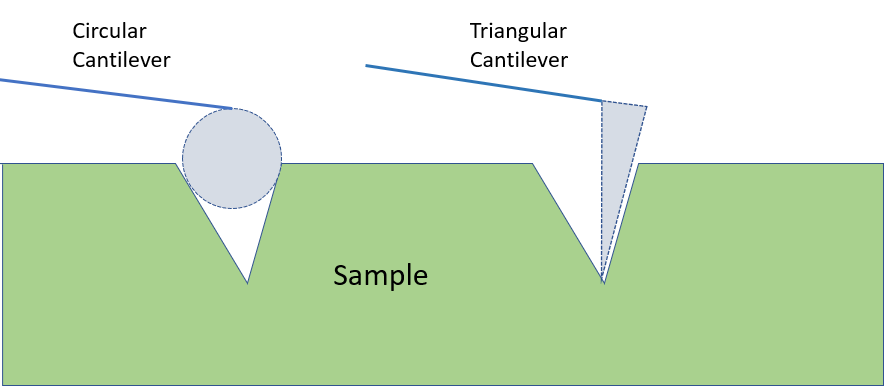
\includegraphics[width=110mm]{chapter2/Tip Shapes.PNG}
\end{center}
\caption{Above is shown the difference between tip shapes and types - where the tip with a circular geometry on the end is unable to enter fully into the crevasse on the sample, the thinner triangular one is. As a result, the output image/data will differ between the two tips, while the underlying structure remains the same, potentially leading the user to incorrectly interpret data.}
\label{fig:tipshape}                 % Reference label to the figure.
\end{figure}

As this tip is brought into contact with the surface it is subjected to various forces. As an example the total force applied to the cantilever is a combination of van-der-Waals attractions and electrostatic repulsion as described in chapter 1. The resultant force scales with the separation distance of the tip from the surface, \textit{h}. When the tip is in direct contact with the surface, the  elasticity of a surface can be directly probed. When the tip is physically in contact with the sample, piezo movement into the surface is directly translated into bending as the cantilever is forced away. This process can also be used to determine the elasticity of surfaces by intentionally pressing the tip into a surface.

For the majority of AFMs in use today, the raw unprocessed data given by a machine boils down to the piezo extension and position of the reflected laser on the photodiode, as well as the piezo's z positional height, which is tied to its total operational range. This data is fed into the feedback control loop in order to adjust the tip's position to stay within operational parameters. This process is tied to the software's main cycle loop time, which occurs faster than the operator can respond to it - on the order of miliseconds, or even less. The operator instead of having a direct involvement in the cantilevers positioning and control instead sets boundaries for a range of variables depending on the operation type, but in general the speed, the force applied to the surface and the operational window (the start distance to intended end distance).

\begin{figure}[h!]     %Insert a figure as soon as possible
        \begin{center}
          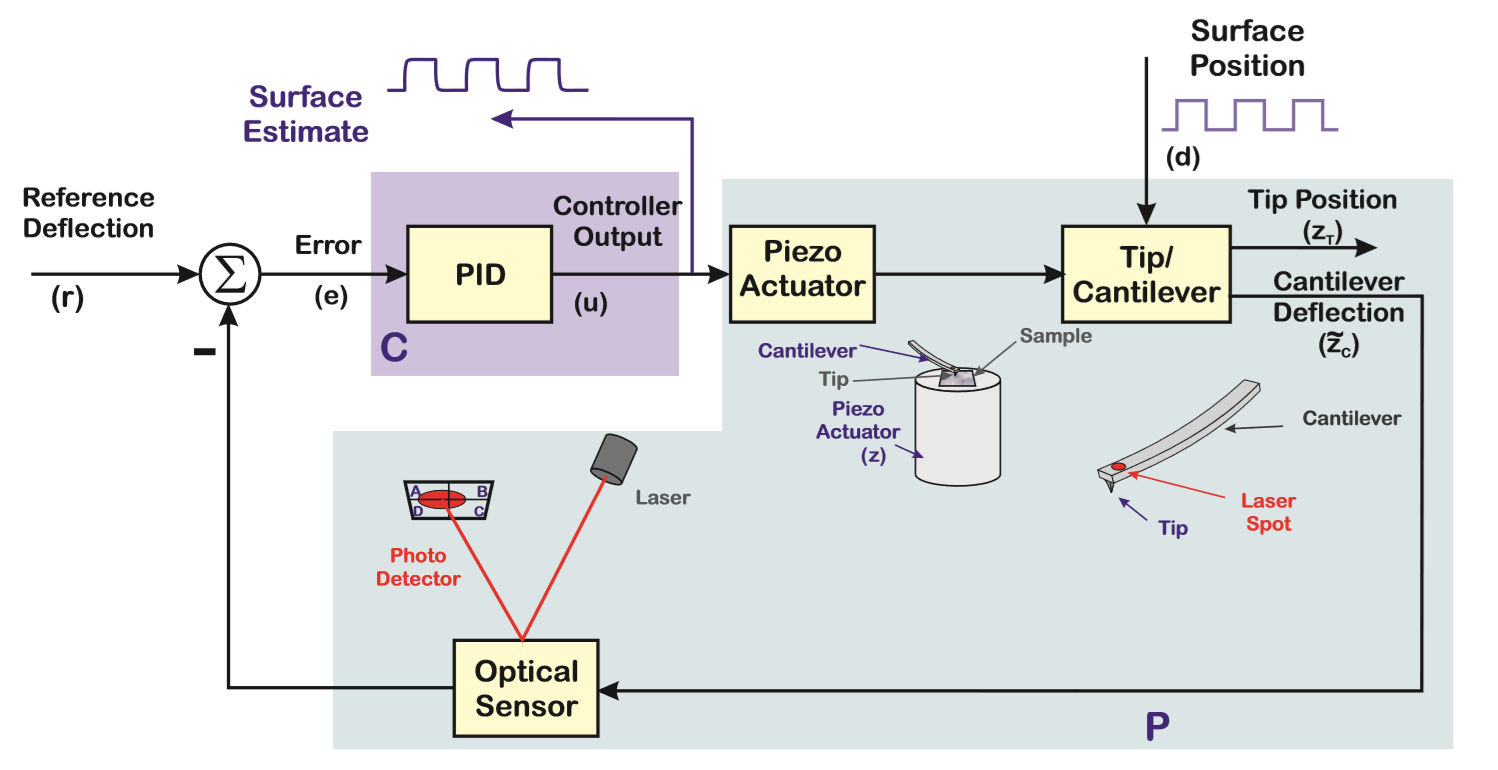
\includegraphics[width=110mm]{chapter2/Feedback.png}
\end{center}
\caption{A diagram demonstrating the basic feedback loop control for an AFM. In this case an example for an AFM operating in imaging scanning mode is shown, which is elaborated in the next section. Image adapted from \cite{AFMTut}}
\label{fig:Feedback}                 % Reference label to the figure.
\end{figure}

From these parameters, the cantilever is controlled in a feedback loop. First a reference signal is generated and cross referenced against the cantilever deflection. From this the gain is tweaked to attempt to apply a constant force to the tip across measurements (known as the setpoint).

%\begin{figure}[h!!!]     %Not needed anymore - too indepth into mechanics.
%        \begin{center}
%          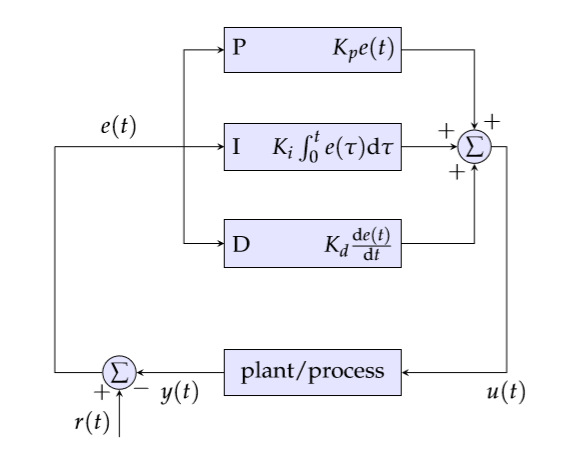
\includegraphics[width=110mm]{chapter2/PID.PNG}
%\end{center}
%\caption{A basic schematic of an PID-controller circuit where \textit{r(t)} is the setpoint, \textit{y(t)} is the reference signal and \textit{u(t)} is the difference. \textit{P} calculates the weight of the error signal input, \textit{I} weights the sum of previous errors and \textit{D} calculates the change in error over time to predict future errors. Image adapted from \cite{GoodAFM}.}
%\label{fig:PID}                 % Reference label to the figure.
%\end{figure}

From this loop, the tip position and the cantilever deflection is recorded. This loop helps to ensure that a constant force is applied to the tip, to reduce tip and sample damage as well as the reduction of errors in the system, as AFMs usually operate at a rate faster than human control. \cite{GoodAFM}\cite{AFMTut}

%The cantilever itself 

Using this loop the tip can then be exposed to various ranges, with corresponding forces acting upon it. These ranges are used to define various modes of operation such as: contact mode; where the tip comes into full contact with the surface, tapping mode; where the tip only lightly grazes the surface and non contact mode; where the tip is only affected by the long range forces. As you move the tip further away from the surface the force applied on the surface is reduced, which is particularly useful for softer samples. For force curves however, the force measured is generally across the spectrum. \cite{GoodAFM}\cite{AFMTut}

\begin{figure}[h!!!]     %Insert a figure as soon as possible
        \begin{center}
          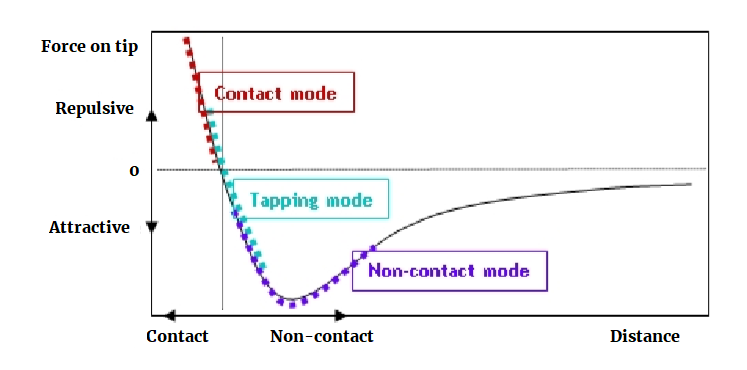
\includegraphics[width=110mm]{chapter2/Regions.png}
\end{center}
\caption{A Van-der-Waals potential with corresponding regions imposed over the curve to demonstrate the ranges each of the modes have in relation to the forces applied to the cantilever. Image adapted from \cite{GoodAFM}.}
\label{fig:Regions}                 % Reference label to the figure.
\end{figure}

For the non-contact modes the probe is set to oscillate at the resonance frequency of the cantilever. When the tip comes close enough to the sample to be affected by the surface forces it causes a dampening of the oscillation, resulting in a phase shift. Using this method, the speed and accuracy of mapping is improved. Tapping mode is similar, except that the nadir of the oscillation is brought into contact with the sample.

From these methods and mechanisms AFM has branched out into performing a range of functions, the two most common being imaging and force profiling which rely on this tip-surface interaction to generate the surface and interaction profiles of samples respectively.

\section{Tip Calibration}
\label{chap:cali}

Tuning a cantilever for use under imaging mode is generally one of the simplest methods of calibrating an AFM. By sweeping a cantilever over a range of drive frequencies a maximum peak of cantilever amplitude can be found. From this the resonance frequency is assumed. However issues can arise when calibrating a tip for use under liquid as the viscous drag of the liquid dampens the oscillations of the cantilever. As a result non contact methods are generally not applicable for imaging samples under a solution and rely on contact methods.

In general however, for cantilevers used in air the thermal noise spectra can be mapped to a simple harmonic oscillator, with a noise floor added to compensate for the baseline noise found in the system. This relies on the cantilever being longer than it is wide, and the the quality factor being greater than the sum of the oscillation. The power spectral density $PSD(\omega)$ as a function of angular frequency is a function that describes how the power of a signal or time series is distributed with respect to frequency.

The $PSD(\omega)$ is used to analyze the cantilever's thermal noise spectrum. The cantilever, when not being externally driven, will still oscillate due to thermal energy (Brownian motion). These thermal oscillations create a noise spectrum that can be analyzed to extract useful information about the cantilever, such as its resonant frequency and quality factor.

the $PSD(\omega)$ is given by:

\begin{equation}
PSD(\omega) = A_{white} + \frac{A_0 \omega^4}{(\omega^2 - \omega^2_r)^2 + \frac{\omega^2 \omega^2_r}{Q^2}}
\end{equation}

where $\omega$ is the Angular frequency, $\omega_r$ is the resonant angular frequency of the cantilever, $A$ is the Peak amplitude of oscillation, $A_0$ is a scaling factor for the peak amplitude, $A_{white}$ is the noise floor, a constant representing the baseline PSD, and $Q$ is the ratio of energy stored to energy dissipated in one cycle. The quality factor is a dimensionless term which correlates to how underdamped said oscillation is - i.e. it is the loss of energy across one oscillation period. 

Generally for imaging mode AFM the thermal tune method of calibration for cantilevers is adequate. One of the major benefits to this method is how it is non damaging to the tip and relies on the thermal energy driving the oscillation of the tip itself in air. From this the spring constant of the cantilever can be detected by using the equipartition theorem which relates the thermal energy of a cantilever to it's spring constant. The output value is then generally sanity checked by cross referencing with the manufacturer's ranges, or in the case of a cantilever created by the operator themselves, a more in depth calibration may be used. Calibration can also be used as a rudimentary method to detect damage to the tip during processing - as degradation of the tip will alter the oscillation of the cantilever leading to results outside of expectations. 

The spring constant of the cantilever is calculated using:

\begin{equation}
\frac{1}{2}k_{B}T = \frac{1}{2}kx^{2}
\end{equation}

Which can be simplified to:

\begin{equation}
k = \frac{k_{B}T}{\langle x^{2} \rangle}
\end{equation}

where k\textsubscript{B} is Boltzmann's constant (1.38064852 × 10\textsuperscript{-23} m\textsuperscript{2} kg s\textsuperscript{-2} K\textsuperscript{-1}) and T is temperature in Kelvin. x\textsuperscript{2} is distance in respect to the power spectral density (PSD), which is fit to the simple harmonic oscillator mentioned above. \cite{ThermalCalc, JankThesis}

\begin{figure}[h!!!]     %Insert a figure as soon as possible
        \begin{center}
          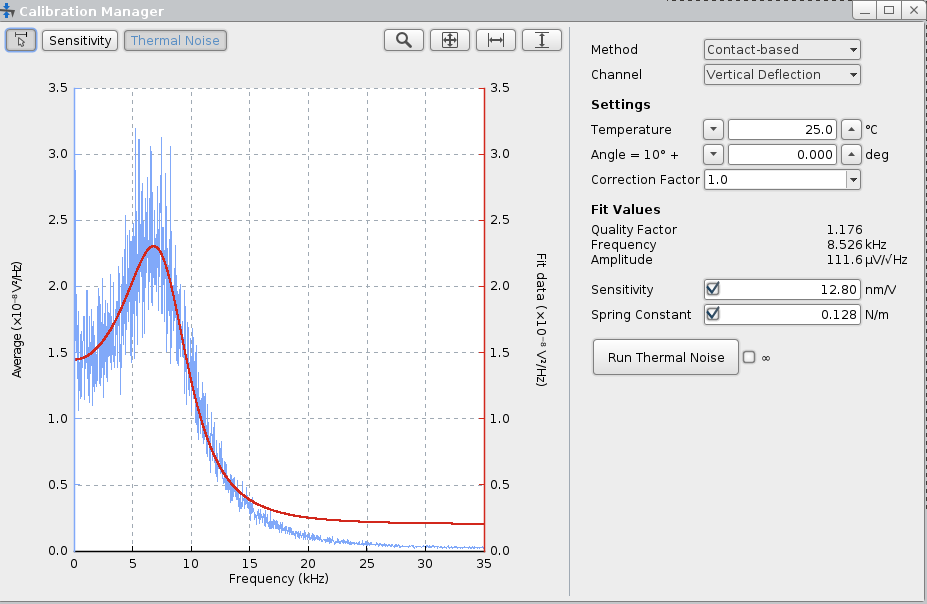
\includegraphics[width=110mm]{chapter2/caliEg.png}
\end{center}
\caption{An example of a thermal tuning calibration software interface.The blue line is the raw signal from the AFM and the red line is the fit over that data. The operation itself is automatic, requiring the user to only press the run thermal noise button for the spring constant to be given.}
\label{fig:caliEg}                 % Reference label to the figure.
\end{figure}

%cite yt vid Tbr8zjLywHI

%Copy paste From wiki do not uncomment: {The quality factor or Q factor is a dimensionless parameter that describes how underdamped an oscillator or resonator is. It is approximately defined as the ratio of the initial energy stored in the resonator to the energy lost in one radian of the cycle of oscillation.}
%Why do people hate defining their terms

After the laser has been aligned the system can detect changes in the cantilever, in particular bending. However, for this bending to be converted into force applied to the cantilever and/or surface, the system itself must be able to translate bending into force. Unlike imaging mode where the peak resonance is the main factor in determining a good calibration, the force instead relies more on a spring constant coupled with the inverse optical lever sensitivity (InvOLS). This is due to the force being calculated, rather than imaging producing a height map based off the cantilever deflection. In the case of force; 

\begin{equation}
F = kz
\end{equation}

where k is the spring constant of the cantilever and z is the cantilever deflection. The cantilever deflection is in turn calculated using:

\begin{equation}
z = InvOLS\Delta V
\end{equation}

Where $InvOLS$ is the Inverse optical lever sensitivity (m/V), and $\Delta V$ is the change in the voltage measured by the photodiode. $\Delta V$ is given as a raw value from the machine.

InvOLS is dependant on a range of different factors such as spot size, position, cantilever length and electronic gains in the system, however this calculation can be bypassed by taking the slope of the curve on a hard surface, then finding the difference needed to convert said slope to be equal to one (Figure \ref{fig:InvOLS}). 

\begin{figure}[h!]     %Insert a figure as soon as possible
        \begin{center}
          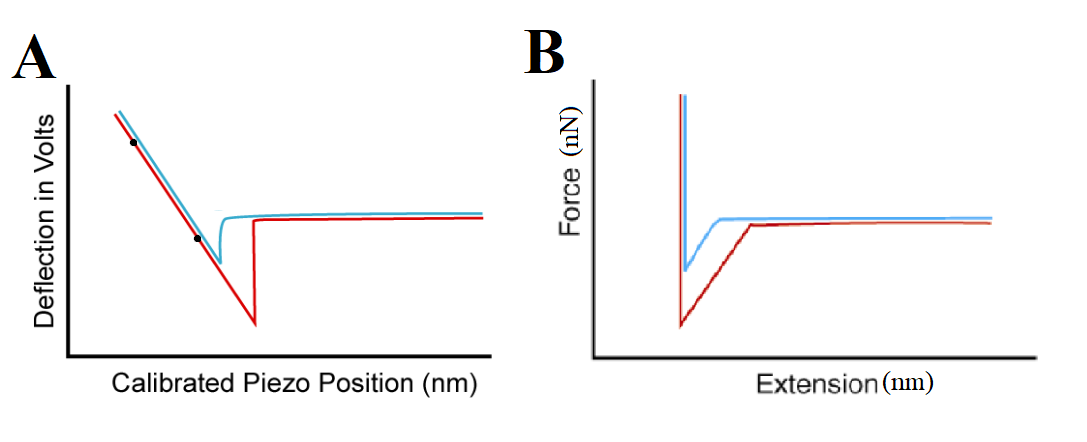
\includegraphics[width=100mm]{chapter2/InvOLS.png}
\end{center}
\caption{A diagram demonstrating the translation of InvOLS to force, A demonstrates the raw data plotted, B demonstrates the data adjusted with InvOLS into a force. Adapted from \cite{AFMTalk}}
\label{fig:InvOLS}                 % Reference label to the figure.
\end{figure}

Both of these methods assume that cantilevers are motionless, or do not contribute any motion to the input motions dictated by the piezo controllers. In reality this is not the case, as cantilevers are always moving. Even a baseline measurement of lever deflection will deviate by 2 nm in vacuums, air and water by thermal noise.\cite{AFMTalk} \cite{AFMCalibration, AFMCalibration2}

%https://nanohub.org/resources/11221/download/2011.02.17-AFM_Workshop-L03-Moshar.pdf

% Add review here. - what review???

%Calibration of the cantilever is required to convert the raw signal produced from the AFM into force data. While an AFM under imaging mode may only need a thermal power spectral density graph plotted

%There are several parameters that can be controlled during force operation that affect the 



%\textcolor{red}{Sader method?}

\section{Common artifacts in AFM}
\label{chap:commonArtifacts}

One of the greatest strengths of AFM can quickly turn into a double edged sword in the wrong hands. Due to how the AFM physically interacts with the surface this means there is a lot more potential for unexpected interaction and unique artifacts when compared with traditional microscopy. Over the history of use of AFM certain recurring artifacts have been identified and recognised. These sources of artifacts in AFM generally come from either the tip, the scanner, vibrations, the feedback circuit, and the image processing software. 

\subsection{The tip}

The geometry of the tip is an important factor in AFM sample preparation and experimental design. this was briefly touched on earlier in figure \ref{fig:tipshape}. However there are further aspects to the geometry that can influence the results. These examples include when the tip itself is either damaged, contaminated or when the tip is dulled from excessive use. A damaged tip will cause an artificial shape up on the surface of the image as seen in figure \ref{fig:BrokenTip}. 

\begin{figure}[h!]     %Insert a figure as soon as possible
        \begin{center}
          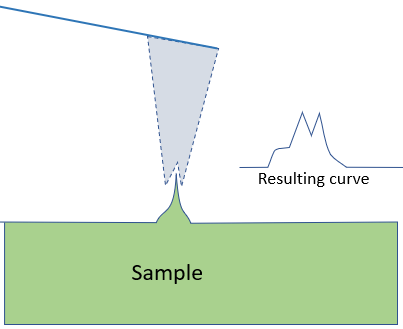
\includegraphics[width=100mm]{chapter2/BrokenTip.PNG}
\end{center}
\caption{As the damaged tip interacts with a sample surface an artificial lump is measured by the cantilever in scanning mode. This is due to the double prong defect in the probe head limiting the range of movement, incorrectly reporting a secondary feature.}
\label{fig:BrokenTip}                 % Reference label to the figure.
\end{figure}

Contaminated tips equally will affect results, but in an irregular way - as contaminants can be gained or lost during an operation. Whilst on a tip they alter the interacting geometry and chemistry of a probe. Additionally, these contaminants can change the surface profile of the sample, leading to inaccurate measurements. For example, if a sample was covered by a contaminant during force profiling, the resulting force curves would be altered by the contaminants interaction with the probe. Contaminants are generally very difficult to remove and usually require some kind of cleaning procedure to remove, hence the use of clean rooms for some sensitive AFM operations.
%this is fluffy - might be better in force curve section

A dull tip from overuse will decrease the sharpness and potentially the length of the tip - essentially widening it's interaction profile. This causes the interacting surface area to widen as well as widening any topology measured by the system. As such it's standard practice to regularly use fresh tips.
%Does this need an image?

Generally these sorts of artifacts provide a repetitive and unusual profile upon the surface, and can be checked by using multiple tips to profile the same sample. If the results are consistent across tips then it's unlikely to contain artifacts created by the tip itself.

\subsection{Scanner error}

The source of scanner error fundamentally derives from the piezoelectic scanner's physical properties. A piezo electric scanner will increase in sensitivity from constant use, or will slowly depolarise and increase in sensitivity when left idle. As a result, piezo electric scanners require regular maintenance to compensate for these effects. In addition to this phenomenon the extension of a scanner in any direction is not linear with its driving signal, which affects all z and x, y movements. When a piezo electric scanner is not properly calibrated this is usually reflected in dimensional distortion in the data. These sorts of artifacts have a constant presence and adjustment to any data generated and as such mandate the proper maintenance of any AFM. 

Correcting for these artifacts is either done by software or hardware and are usually not performed by the operator, instead handled by the manufacturer. Though nonlinearity effects are much less pronounced on the Z axis due to the reduced range of movement and these sort of effects only matter for very precise measurements when height profiling. 

Hysteresis is also a consideration when AFMs are cyclically scanned across a profile - these can cause a lateral shift along a trace and retrace curve causing an asymmetric step height. In the same vein rows can have drift, though this is due to a disconnect between in time steps between voltage driving movements. This usually presents itself as a bending drift across rows shown in figure \ref{fig:Creep}. Equally, this is why "zooming" into a scanned profile is difficult - these effects will displace the frame of reference by a certain offset when moving due to the change in cantilever scan velocity. 

\begin{figure}[h!]     %Insert a figure as soon as possible
        \begin{center}
          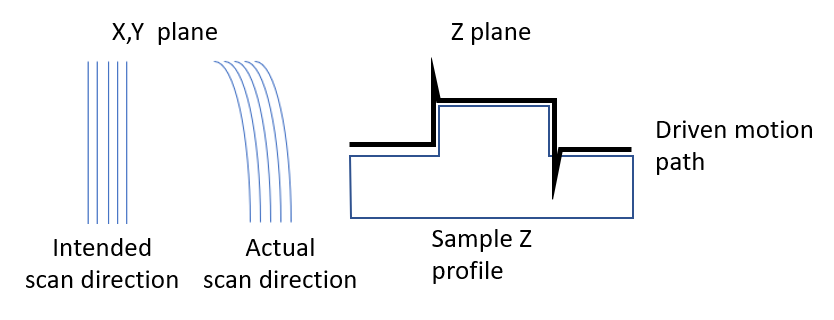
\includegraphics[width=100mm]{chapter2/Creep.PNG}
\end{center}
\caption{Creeping drift can occur across the motion of a scan. In the x, y direction this manifests as a bending motion, whereas in the z plane this can result in an overshoot of driven motion. In both cases the effects are exaggerated to convey the effects.}
\label{fig:Creep}                 % Reference label to the figure.
\end{figure}

%Too much detail - simplify? Maybe just spam images

In some cases of AFMs there is a parabolic arc attached to the x and y axis component of the piezo movement, which will cause bowling in the resultant image. Additionally, the sample itself cannot be atomically flat when inserted into the AFM. These two effects combine to cause an intrinsic tilt on the resultant image.

Finally thermal drift can cause changes in physical properties which will cause deviations from a thermally calibrated cantilever and the new properties. In the case of high resolution images small areas of thermal flux can cause issues, requiring the operator to wait until thermal equilibrium is reached.

The majority of these effects are dealt with either by hardware/software compensations outside of the standard use of AFM. During the data interpretation phase several mathematical transformations are performed on the data set to adjust for these effects.

\subsection{Vibrations}

Vibrations in the building, either due to foot traffic, wind, or even speech can cause physical displacements between the tip and sample. These vibrations can cause sudden shifts in the trace/retrace profile of a cantilever - leading to dramatic changes in the data. These are relatively easy to isolate as one time events however, and can be managed by operating the AFM in a quiet room with minimised background noise.

\subsection{Incorrect user parameters and feedback errors}

A large part of the AFM operation relies on the user to correctly set parameters during use. Generally these parameters are concluded during the operation to ensure that the output images are satisfactory. If incorrect parameters are set, then erroneous results can be easily produced. For example soft samples' profiles may be incorrectly compressed from a contact force too high, leading to a shorter than true height. As part of the feedback and correction mechanism relies on these input parameters the automatic corrections can further conflate errors in the resulting dataset.

For the majority of cases these artifacts are ironed out and compensated for over the course of sample familiarisation and as a result AFM tends to have a higher difficulty curve when compared to other microscopy techniques. Whereas other microscopy techniques will generally provide some sort of visual representation the sample imaging, improper use of AFM can result in phantasmagorical images without the appropriate care and consideration, leading to incorrect conclusions. \cite{AFMBook1}
%I really like the use of phantasmagorical here, but will it survive the review process?



%This whole section is spotted throughout with the orange book - cite it


\section{Imaging mode AFM}

Imaging mode focuses on using the AFM operation to measure the z-height of a sample across an x, y scan range. The positions are recorded in a three dimensional array, with the distance between each x, y entry value being constant. The major operation is much the same as described above, with the requirement of a piezo controlling x, y movement as well as z movement. The surface of the sample is imaged across using a raster pattern. This raster motion attempts to keep the respective z height at a specific force/deflection value as it progresses along the surface. In the case of non contact or tapping methods the oscillation dampening effect is kept constant across each position. The resultant array is often converted mathematically into a height map to display the surface profile of the imaged sample. 

Some AFM setups also provide other images during scanning; a phase image, an amplitude (or deflection) image and a friction image depending on the operational mode of the AFM. Generally two operational modes are available for the operator; contact and non-contact mode. Contact mode physically brings the tip in contact with the surface, then drags it across the surface. This is useful for measuring friction, reducing current effects on the tip in a liquid AFM situation and physically interacting with surface objects on the nanoscale. However this does have a shear force effect on the sample, and can damage particularly sensitive samples, such as biological material. Non-contact mode oscillates the cantilever above the surface, only allowing the tip to touch the surface gently at the nadir of the oscillation. By subtracting the input oscillation from the physical oscillation of the cantilever the phase can be determined. This indicates the softness of a surface, as harder surfaces dampen the movement to a greater degree, reducing the angle of the reflected laser.

\begin{figure}[h!]     %Insert a figure as soon as possible
        \begin{center}
          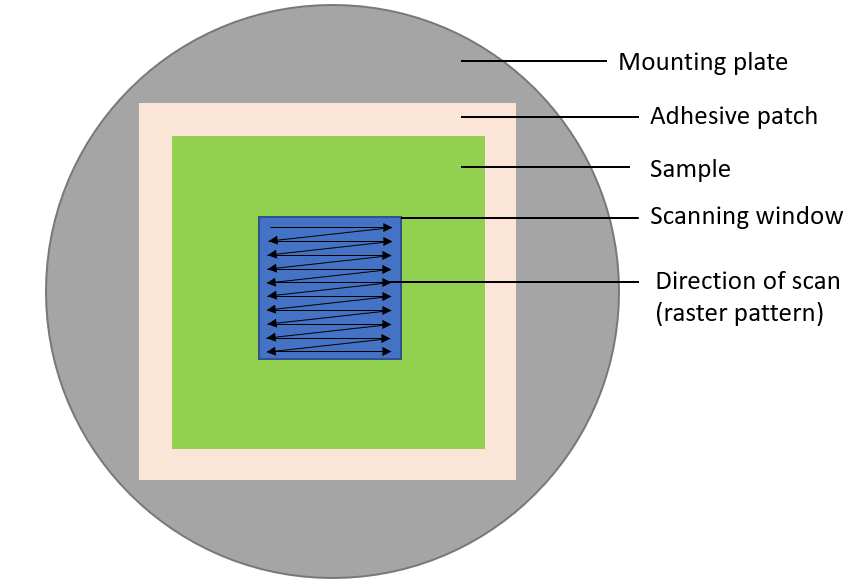
\includegraphics[width=100mm]{chapter2/SampleExample.PNG}
\end{center}
\caption{A diagram demonstrating the model setup for a sample. The geometry of each of the layers in the sample setup is an example in this case and can vary with application and requirements. The scanning window is non physical and is a projection of the area scanned by an AFM upon the surface of a sample.}
\label{fig:SampleExample}                 % Reference label to the figure.
\end{figure}

During use the operator defines a field of view (aka the scanning window) -  a range of coordinates that the AFM will take points of. This field of view is then broken up into number of points per line, which defines the aforementioned distance between each data point.

The raw export data is generally saved as a file, either to be adjusted in software or externally. This final data export however isn't reflective of the surface profile yet however - as the geometry and the local angle of the surface will alter the resultant output array. To compensate for the drift in the AFM and for the angle of the surface below the cantilever probe a few mathematical transformations are generally applied.

\subsection{Mathematical alignment and error correction of AFM images}

The use of AFM has proliferated across the sciences due to its wide range of applications and data output. However in some cases the image produced is assumed to perfectly reflect the surface of the sample, when in reality there are a number of mathematical, physical and operational effects that can vastly affect the output image. Mathematical transformations are applied to the raw data via image processing. Physical errors can occur from the situations the tip is exposed to and the condition of the tip. Finally operational errors can occur from improper use. As a result it is important to consider where these transformations and errors can arise to ensure that the image produced from the machine is a reflection of the true surface of the sample.

A part of the image processing process is done to compensate for the unavoidable artifacts discussed in \autoref{chap:commonArtifacts}. However this can be a source of error itself, as over reliance on multiple correction methods can introduce artificial profiles into the image. Other filters, such as a low pass filter can smooth out or remove sharper features in a data set. As such it is important for the operator to justify and consider any transformations upon the underlying data set.

%Example of "bad" paper with obvious tip defects/poor analysis? Can I even call out people like that?

\begin{figure}[h!]     %Insert a figure as soon as possible
        \begin{center}
          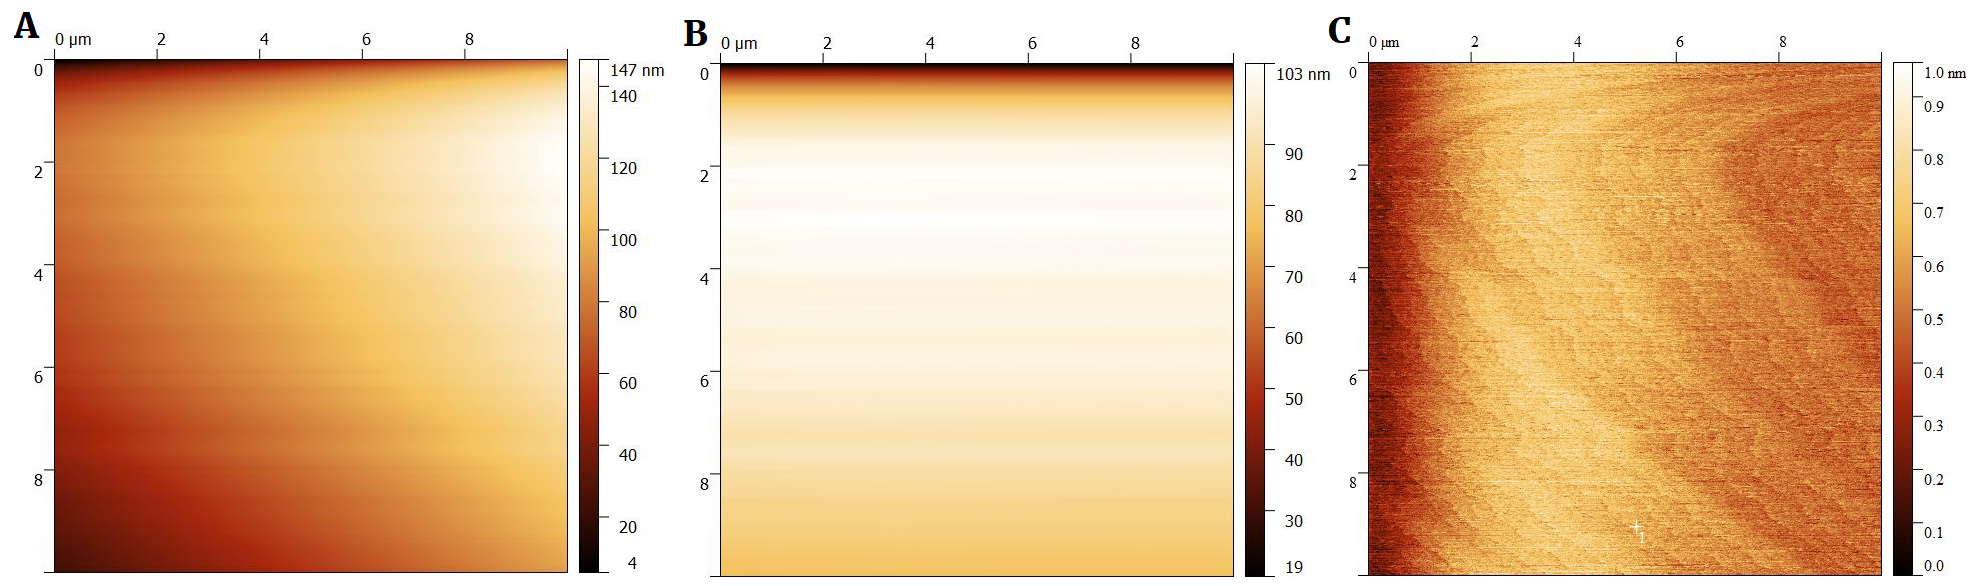
\includegraphics[width=140mm]{chapter2/MathOp.png}
\end{center}
\caption{A figure demonstrating a standard mathematical operation applied to raw data. A demonstrates the array shown direct without any processing, B has had a mean field plane subtraction applied and C has had a row alignment applied to it. The image itself is of a freshly cleaved mica surface which is reflected in the final image C.}
\label{fig:MathOp}                 % Reference label to the figure.
\end{figure}

Mathematical operations are performed on all images as the data generated does not account for the tilt of the surface, therefore a degree of mathematical transformation is required. Initially a heatmap of the the output will look similar to Figure \ref{fig:MathOp}. A mean field plane subtraction is used to determine the plane on which the data was generated, this is then removed across the dataset. This is to normalise the raw height data on a theoretical flat plane as an attempt to remove the tilt present on the sample stage. Next the rows of data are aligned by taking the representative height of each row and aligning each row to that height, this is done by several different methods, such as polynomial or median methods. As a result the features on the surface of a sample are kept intact, but it is possible that sharp differences observed on a row by row basis can be obfuscated due to image processing. The size of a pixel is dependant on the scan size (for example a 10$\mu$m by 10$\mu$m image with 512 data points per line means that each pixel is approximately worth 20 nm). Though, this does not represent the interacting surface area between the tip sample surface. In order to reduce errors like these and to resolve features that may be hidden by pixel weight larger scan sizes are often coupled with smaller scan sizes to give both the larger order topography with the smaller detail analysis. It is important for an user to not perform too much image processing without explanation and reasoning as each additional correction can be a further abstraction from the truth.

\begin{figure}[h!]     %Insert a figure as soon as possible
        \begin{center}
          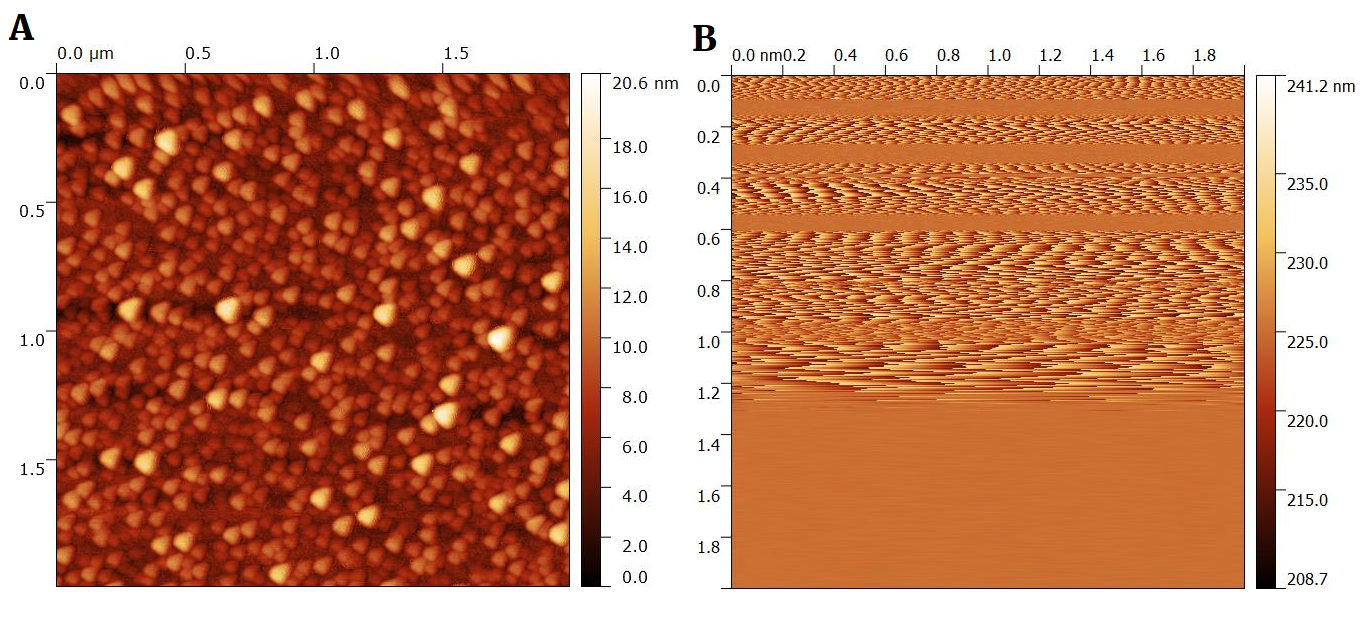
\includegraphics[width=140mm]{chapter2/Error.png}
\end{center}
\caption{A figure demonstrating different errors and operations on the output images produced from an AFM.  A.  demonstrates  a  physical  complications produced by contaminants on tip damage.  B. highlights an example of the zigzag patterns that can be produced from operation error, as well as the blank areas where the tip is not in contact with the surface.  }
\label{fig:Errorr}                 % Reference label to the figure.
\end{figure}

Another consideration with AFM is that since the image is scanned over time rather than instantly there is a degree of physical error introduced during operation. Thermal fluctuations, piezo-error, vibrations and air fluctuations. Generally the error of an AFM in imaging mode is given to be +/-1 nm on the x and y length scale and +/-1 \AA{}ngstrom on the z length scale. Issues are made worse within liquid conditions where current effects induced by probe movement, vibrations, sample setup and approaching the surface can frustrate results. The change in refractive index in the liquid means that the laser has to be realigned and re-calibrated in more difficult conditions. Additionally it is important to assess images produced for unusual mechanical errors, such as the double tip effect, where the tip becomes damaged during scanning and the defect in the tip's geometry is reflected onto a sample. There runs the risk of papers being published with potential double tip effects within their AFM analysis to an unknowing operator, the double tip effect is shown in Figure \ref{fig:Errorr}.A.

The operator is able to adjust several variables whilst operating an AFM. How much force is exerted on the surface as a result of the tip's proximity is altered; too light and the output image is unclear, but  increasing force causes increased tip degradation rate. The scan rate is how fast the AFM scans, faster speeds increase image production, reducing the effects of drift, piezo error and thermal fluctuations. However, a high scan rate can result in unclear images and an increase in tip degradation. Finally gain can be adjusted, the values of which vary on the sample, setup and device. Images produced with incorrect settings can result in wavy mechanical patterns or poor image quality. An example of a tip that hasn't engaged the surface properly, therefore resulting in a poor pattern is shown in Figure \ref{fig:Errorr}.B. \cite{AFMBook2, AFMBook1}

%HMM maybe move house of horrors before
\section{Surface Force profiling}

Force microscopy operation of an AFM differs from imaging mode in that the x, y movement of the piezo is removed, and instead a static sample is placed underneath, with several curves taken of a single site. This uses the mechanical nature of AFM to quantify forces applied upon the tip of the cantilever. These forces cause the cantilever to bend away in the event of repulsive forces, or towards the surface in the event of an attractive force. The interacting surface chemistry and profiles of both the tip and sample determine these force interactions. This contact area is also influenced by the solution that this area is immersed in, such as ions within the solution screening charges between the two profiles.

Having an accurate spring constant of the cantilever is paramount for these kinds of operations, as the measured parameter is the deflection of the cantilever reported by the photo diode. This can be then translated into force using the calibration methods discussed in section \ref{chap:cali}. This is one of the reasons why calibration is still performed for manufactured tips with given spring constants.

\subsection{Anatomy of a force curve}

A force curve is fundamentally the force ``felt" by a cantilever as it is moved along a z axis. From this seemingly simple motion, several events commonly occur across this simple motion. 

\begin{figure}[h!]     %Insert a figure as soon as possible
        \begin{center}
          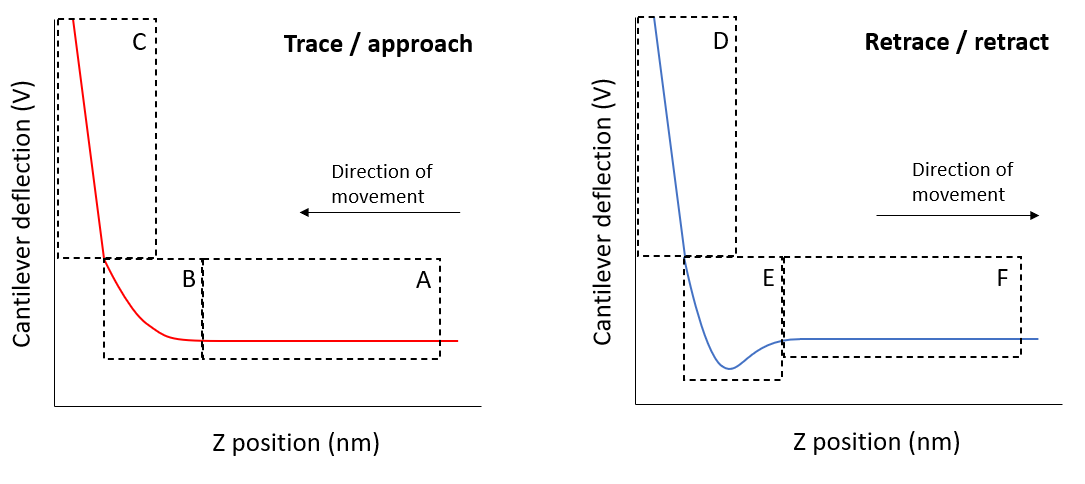
\includegraphics[width=140mm]{chapter2/forceCurveAnatomy.PNG}
\end{center}
\caption{A diagram showing a model force curve event. The leftmost image corresponds to the trace (aka approach) curve the first part of the force profiling event. The trace force curve proceeds from the bottom right up to the top left, passing through the A,B and C events in order. After this motion the piezo movement reverses, retracting the cantilever away from the surface, this begins the start of the retrace curve. In reverse fashion the cantilever progresses through the D,E and F sections in order.}
\label{fig:forceAnatomy}                 % Reference label to the figure.
\end{figure}

Given above in figure \ref{fig:forceAnatomy} is an unprocessed model force profile across one single scan. The first event labelled as A is the approach part of the curve - where the tip and sample are too far away for any forces to be detected by the cantilever. When the surface begins to apply force upon the cantilever it enters phase B; where the curve begins to bend away. This bending is indicative of a repulsive force between the two surfaces. When the cantilever is finally brought into contact with the surface the curve transitions into a linear profile, where any z movement is directly translated into deflection. The tilt intrinsic to this phase can be transformed away by converting deflection into force given in section \ref{chap:cali}.

In some cases it is possible for the operator to set a delay time to retain the tip upon the surface of a sample between the two curves. This is known as a delay period. Afterwards the retrace curve follow the same pattern a the trace, but in reverse, going through D,E,F. Region E indicates an attractive force between the sample and tip, bending the tip downwards. As these sample-tip bonds break the cantilever will snap up from the stress applied from bending. This can cause multiple snap up events if the interacting surface can unfold.

\newpage

\subsection{Error correction of force curves}

Since force profiling is restricted to a single axis in movement, the potential for error is reduced. The majority of artifacts and errors come from contaminants in the system, tip defects, or incorrect operational parameters. of particular note any error incurred by scanner artifacts such as drift is reduced when compared to imaging from the reduced dimensionality. Though one additional aspect does influence results that does not affect imaging mode - the relative topological differences between the interaction areas aka roughness. \cite{TipRoughness}

\begin{figure}[h!]     %Insert a figure as soon as possible
        \begin{center}
          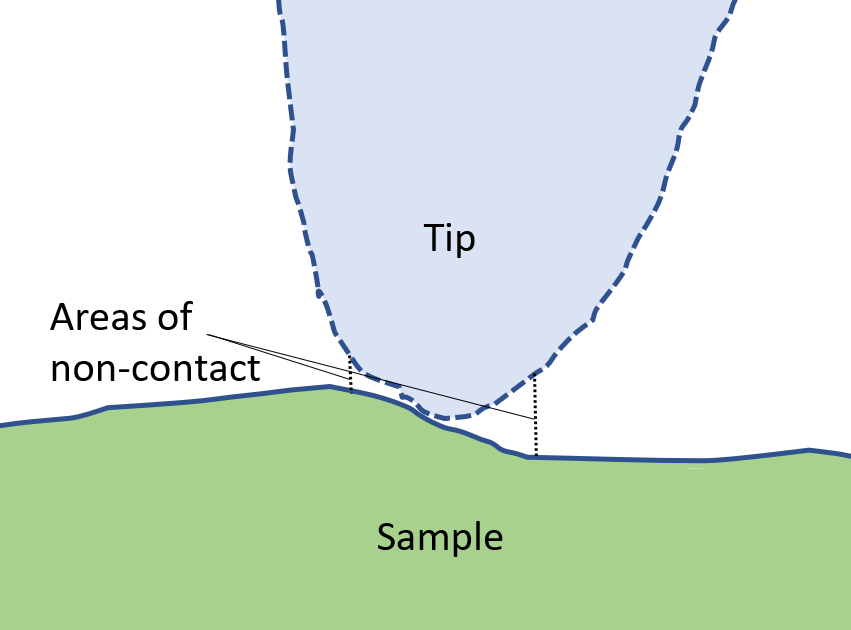
\includegraphics[width=100mm]{chapter2/tip contact.PNG}
\end{center}
\caption{A theoretical demonstration of a rough AFM tip interacting with an imperfect surface. Due to the differences in topology between the two surfaces the interacting areas generate a different sum force experienced by the tip than expected.}
\label{fig:tipCont}                 % Reference label to the figure.
\end{figure}

These differences can cause the sum force applied on the tip to be different than expected, leading to an adjusted force curve. This is due to the DLVO force profile resulting in different force effects along the different points within the contact area as shown in figure \ref{fig:tipCont}.
%Need better reference

In addition to this, because of the unstable geometry of the local area, as driving force increases, forcing the cantilever further into the sample, the tip itself can slip along the surface into a new more stable minima along the profile. This can cause sudden changes in the C/D regions mentioned in figure \ref{fig:forceAnatomy}. This effect is described in figure \ref{fig:tipSlip}. \cite{Ahmad2015}

\begin{figure}[h!]     %Insert a figure as soon as possible
        \begin{center}
          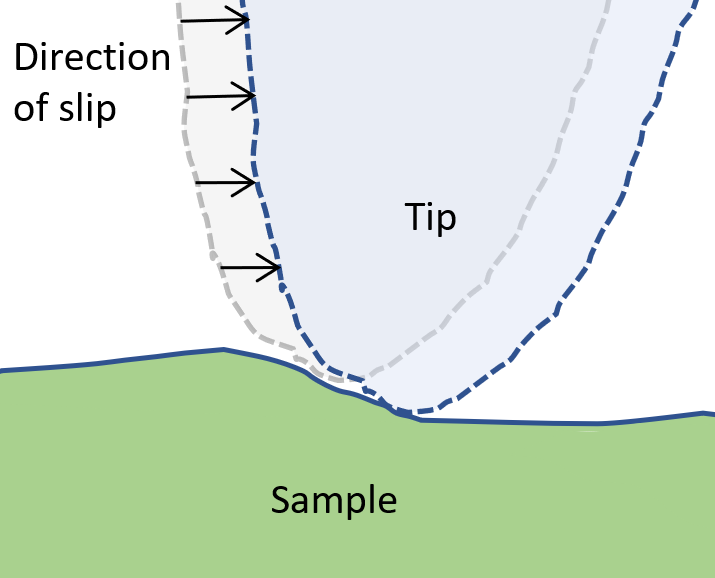
\includegraphics[width=100mm]{chapter2/tipslip.PNG}
\end{center}
\caption{A demonstration of the theoretical movement that a cantilever tip will undergo when slipping along a surface profile.}
\label{fig:tipSlip}                 % Reference label to the figure.
\end{figure}

To deal with these effects multiple force curves are generally taken across a range of sites to ensure that any localised profiles are averaged out.

One other consideration is the effects of hydrodynamic forces which will has a constant effect on the tip during motion (phases A/B and E/F in figure \ref{fig:forceAnatomy}). This only is present in samples immersed in a liquid, and generally doesn't impact the final curve too much. This effect can be profiled by running the machine in different driving speeds.

One other effect upon the resulting data profile is the driving speed of the cantilever during profiling. Depending on the measuring tick rate some nuance to the data can be smoothed out as a faster speed will have less time to measure each point in the curve. An operator will generally tune the machine and setup to find an acceptable middle ground between data points and time taken.\cite{AFMSurfaceProfile}
%Expand with a general overview


%\section{Application of Derjaguin approximation}
%moved to chapt 1



%AFM imaging
% Need more detail on attempts to clean/reduce dust on surfaces
%Need plasma images if possible (Or talk about how they didn't work)
%Need JPK images
%
\chapter{Surface Imaging}

\section{Introduction}

Atomic force microscopy (AFM) is a powerful tool for surface imaging, providing high-resolution topographical maps of sample surfaces. This technique is pivotal for understanding the morphology and texture of materials at the nanoscale. In this study, AFM was employed at various stages to quantitatively analyze the surface roughness of different materials.

\begin{figure}[h!!!!!!!]     %Insert a figure as soon as possible
        \begin{center}
          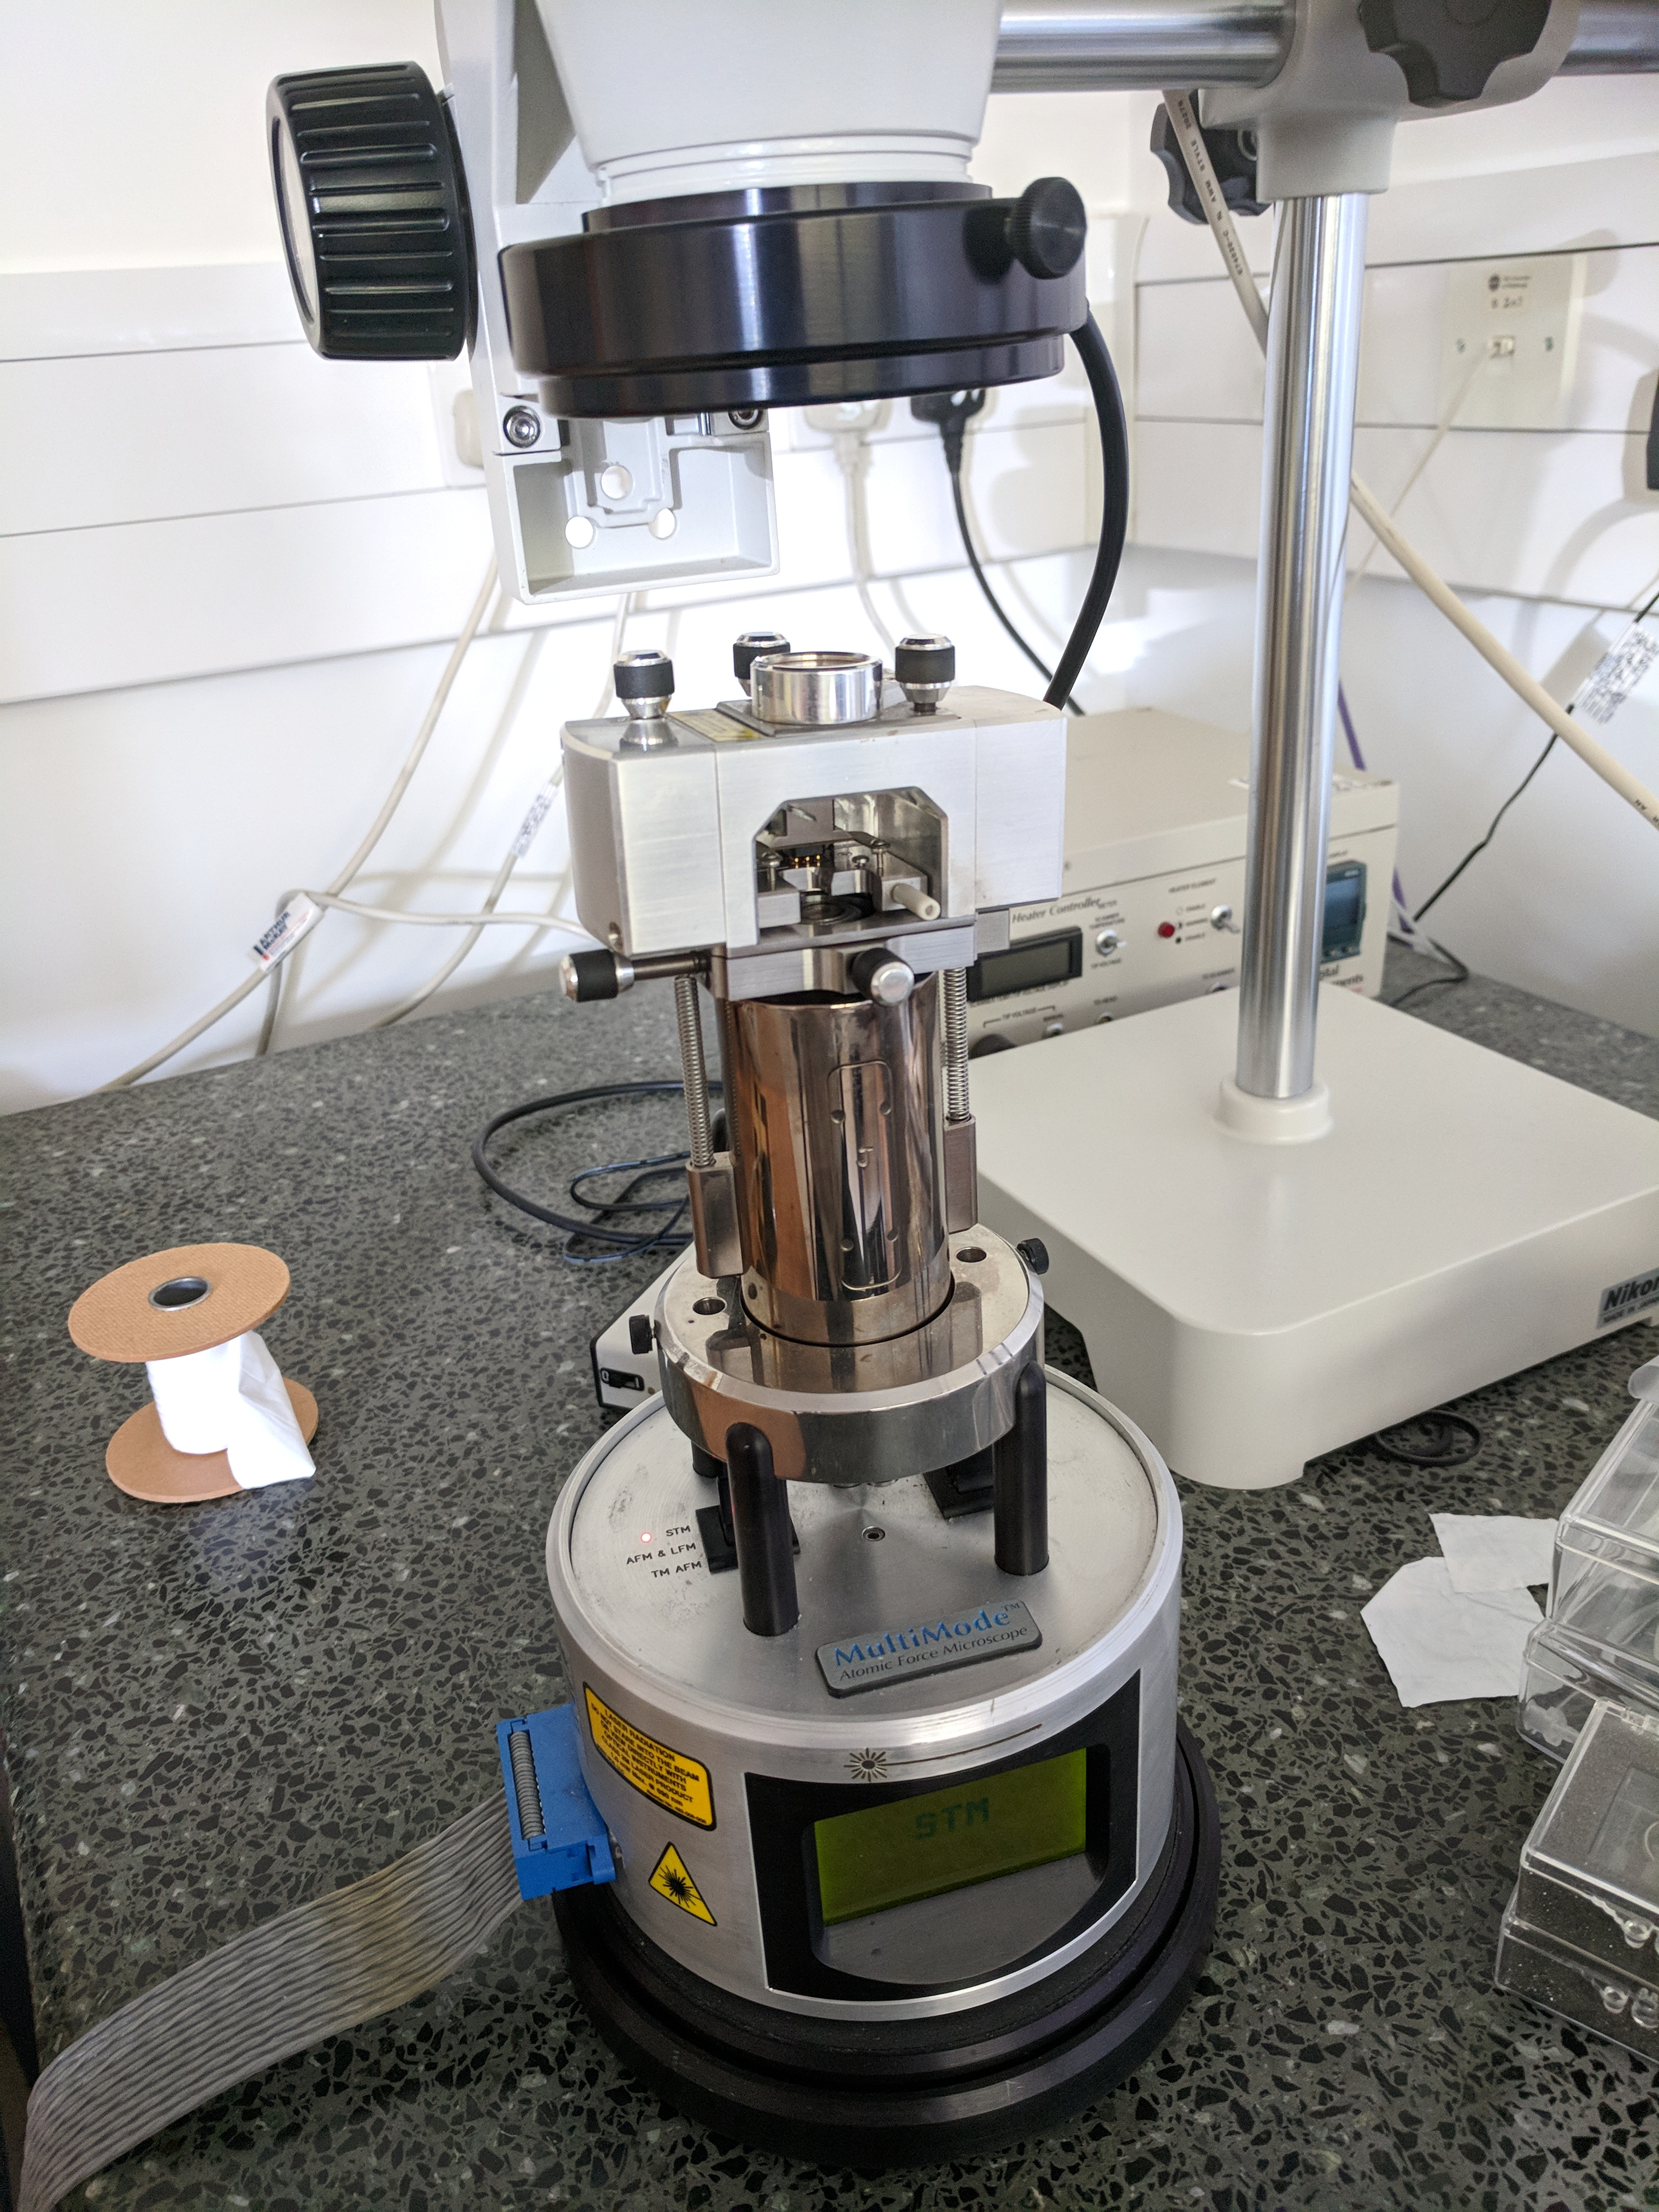
\includegraphics[width=70mm]{chapter2/ImageAFM.jpg}
\end{center}
\caption{Photograph of the operational setup for the Bruker Nanoscope 2, which was used for image measurements.}
\label{fig:ImageAFM}                 % Reference label to the figure.
\end{figure}

For the imaging purposes, we utilized the Bruker Nanoscope 2 AFM system shown in \ref{fig:ImageAFM}. This system is designed with a sample stage capable of securing a 1cm disc, integrated with the J scanner piezoelectric stage for precise movement. The optical alignment of the laser onto the cantilever is achieved using a finely adjustable mirror mechanism, with the head unit being stabilized by tension springs to ensure accurate tracking of surface contours.

\section{Surface analysis}

\subsection{Measuring the surface of mica}

In order to assess the capabilities of the AFM a freshly cleaved mica surface was scanned under the AFM. As mica is assumed to be atomically flat \cite{MicaSurf, Ostendorf_2008}. The cleavage of mica along its basal plane typically results in a smooth and featureless topography, making it an ideal substrate for AFM calibration and analysis.

\begin{figure}[h!!!!!!!]     %Insert a figure as soon as possible
        \begin{center}
          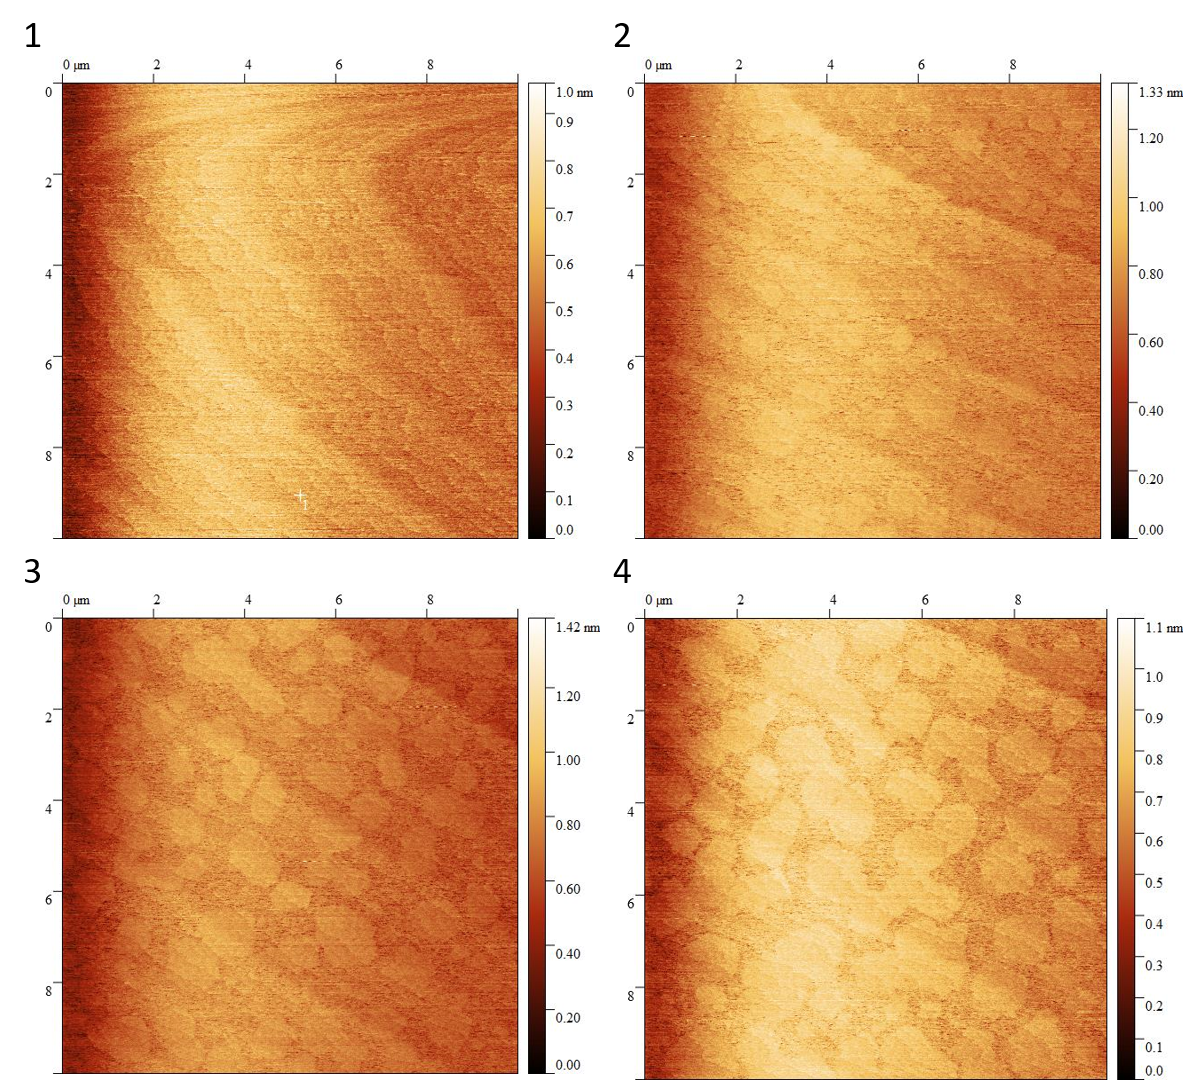
\includegraphics[width=110mm]{chapter3/Mica hydration.png}
\end{center}
\caption{Time-lapse AFM tapping mode images of a mica surface showing progressive hydration. The first image was taken roughly 10 minutes after cleavage, with each subsequent image taking about 30 minutes to take. The changes in surface texture and color intensity suggest the absorption of water from the air, leading to a more pronounced hydration pattern, as seen in the increased contrast and the development of distinct features over time.}
\label{fig:ImageAFM}                 % Reference label to the figure.
\end{figure}

When a mica surface is freshly cleaved and exposed to air, it is expected to present an initially smooth and flat surface at the atomic level due to its layered crystalline structure, which allows for easy cleavage along the basal plane. However, when exposed to ambient air, the mica surface can begin to adsorb water molecules due to its hygroscopic nature, leading to the formation of a hydration layer. This process is gradual and can be observed as an increasing surface roughness or the development of hydration-related features in AFM images over time. The images you've provided suggest such a hydration process, as indicated by the visual changes that become more pronounced with time, which is consistent with the behavior of mica in a typical laboratory environment with moisture present in the air. \cite{MicaSurf, MicaHgryo, Koishi2022WaterAdsorption}

\subsection{Silica Surface Analysis}

 One common sample that was regularly imaged across the entire investigation was silica, be it a silica sphere or borosilica glass surface. A range of different types of silica surfaces was investigated as well as surface treatment techniques performed on the same glass surface. Initially borosilicate glass capillaries were investigated. This investigation intended to resolve the uniformity of a borosilicate capillary across multiple capillaries by profiling the surface topology and roughness across a range of different points. This glass capillary was then cross referenced against the petri dish in use, to ensure that the surface of the petri dish was representative of borosilicate glass. This surface was then referenced against scanning electron microscopy images of the tips, alongside inverted AFM imaging of the tip.

Initially the inside of a glass capillary was imaged. The inside of the capillary was imaged by scoring the glass with a diamond tipped pen, with pressure applied on the outside to break the glass cleanly open \ref{fig:figure8}. This glass reference was used as a representation for the borosilica glass roughness used in Chapter 4 and 8, as the petri dish used in chapter 4 was too large to fit into the AFM.

\begin{figure}[h]     %Insert a figure as soon as possible
        \begin{center}
          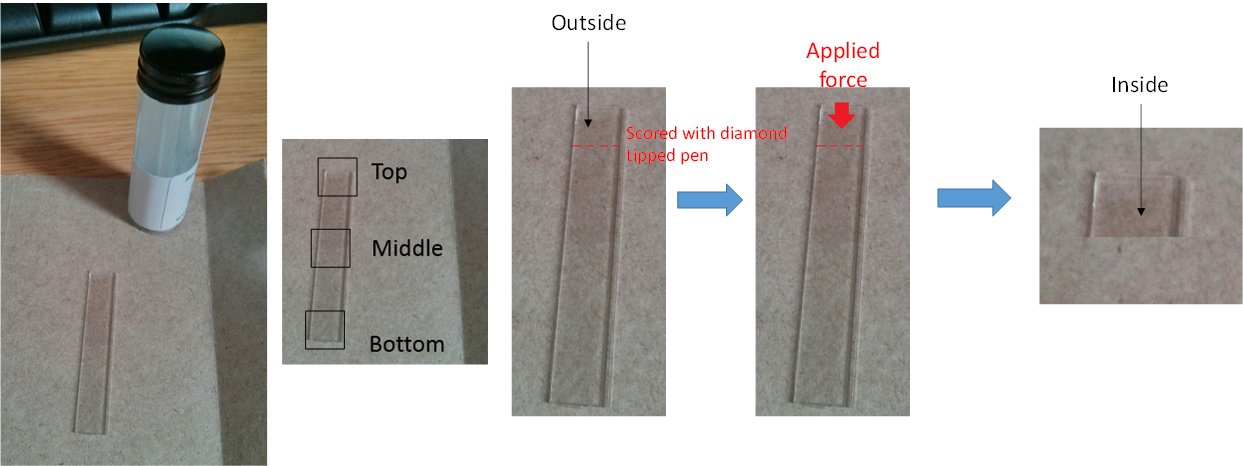
\includegraphics[width=120mm]{chapter3/Figure8.png}
\end{center}
\caption{A diagram demonstrating how the glass capillary was broken and how samples were extracted from the capillary.}
\label{fig:figure8}                 % Reference label to the figure.
\end{figure}   


The sample was then loaded inside up into the AFM under tapping mode operation in air. Multiple antimony doped silicon tips (Bruker RFESP-40 tips) were used to scan several samples each, giving a range of tips used for imaging. This was done to reduce any tip artifacts or degradation of tips so that image quality was retained throughout. A constant scan rate of 0.4Hz across all samples with the integral and proportional gain determined using the initial sample, then kept constant at 0.22 and 0.63 respectively. This was done to produce images that were similar as possible to one another from a parameter point of view. Large hysteresis effects present in the pizeo was negated by a small dummy scan window, where the AFM was left to run for a few seconds then reset to the origin of the scan. Each capillary was imaged 12 times at a 10$\mu$m x 10$\mu$m scan size followed by a 2$\mu$m x 2$\mu$m scan size. Images were taken at the top, the middle and the bottom of the capillary with a repeat image taken per site. Finally, two capillaries were imaged giving a total of 24 images. Scan sizes were chosen to give a larger view of the surface, while also scanning an area similar in size to the cantilever head used during the preliminary exploratory experiments (1.6$\mu$m x 1.6$\mu$m). The bead size was later increased to 6.6$\mu$m during the course of the exploration, representing the final dataset (see chapter 4). 

In the case where dust was present in the images, to allow the applicability of a wider dataset, a standard method was used to handle dust. This involved two steps: image processing and visual inspection. After mean plane subtraction to correct for image tilt and alignment using a 5th order polynomial transformation, the images are closely examined. Dust is recognized by its consistency across all open-air images. To isolate and remove dust from the analysis, the z-axis range is adjusted, effectively minimizing the prominence of the dust in the visual representation. This method enhances the clarity of the underlying surface topology in the resultant images. Dust was only present in a small selection of the images.

\begin{figure}[h]     %Insert a figure as soon as possible
        \begin{center}
          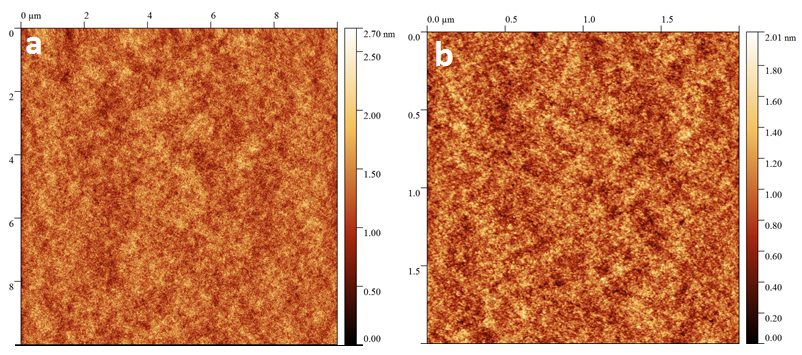
\includegraphics[width=120mm]{chapter3/Figure9.png}
\end{center}
\caption{Two sample AFM images of untreated borosilicate glass at two different scan sizes: (a) displays an image with a scan size of 10$\mu$m x 10$\mu$m, while (b) demonstrates a scan size of 2$\mu$m x 2$\mu$m.}
\label{fig:figure9}                 % Reference label to the figure.
\end{figure}   

\newpage
\subsubsection{Results}

The images for the top part of the glass are shown below:

\begin{figure}[h!!!!]     %Insert a figure as soon as possible
        \begin{center}
          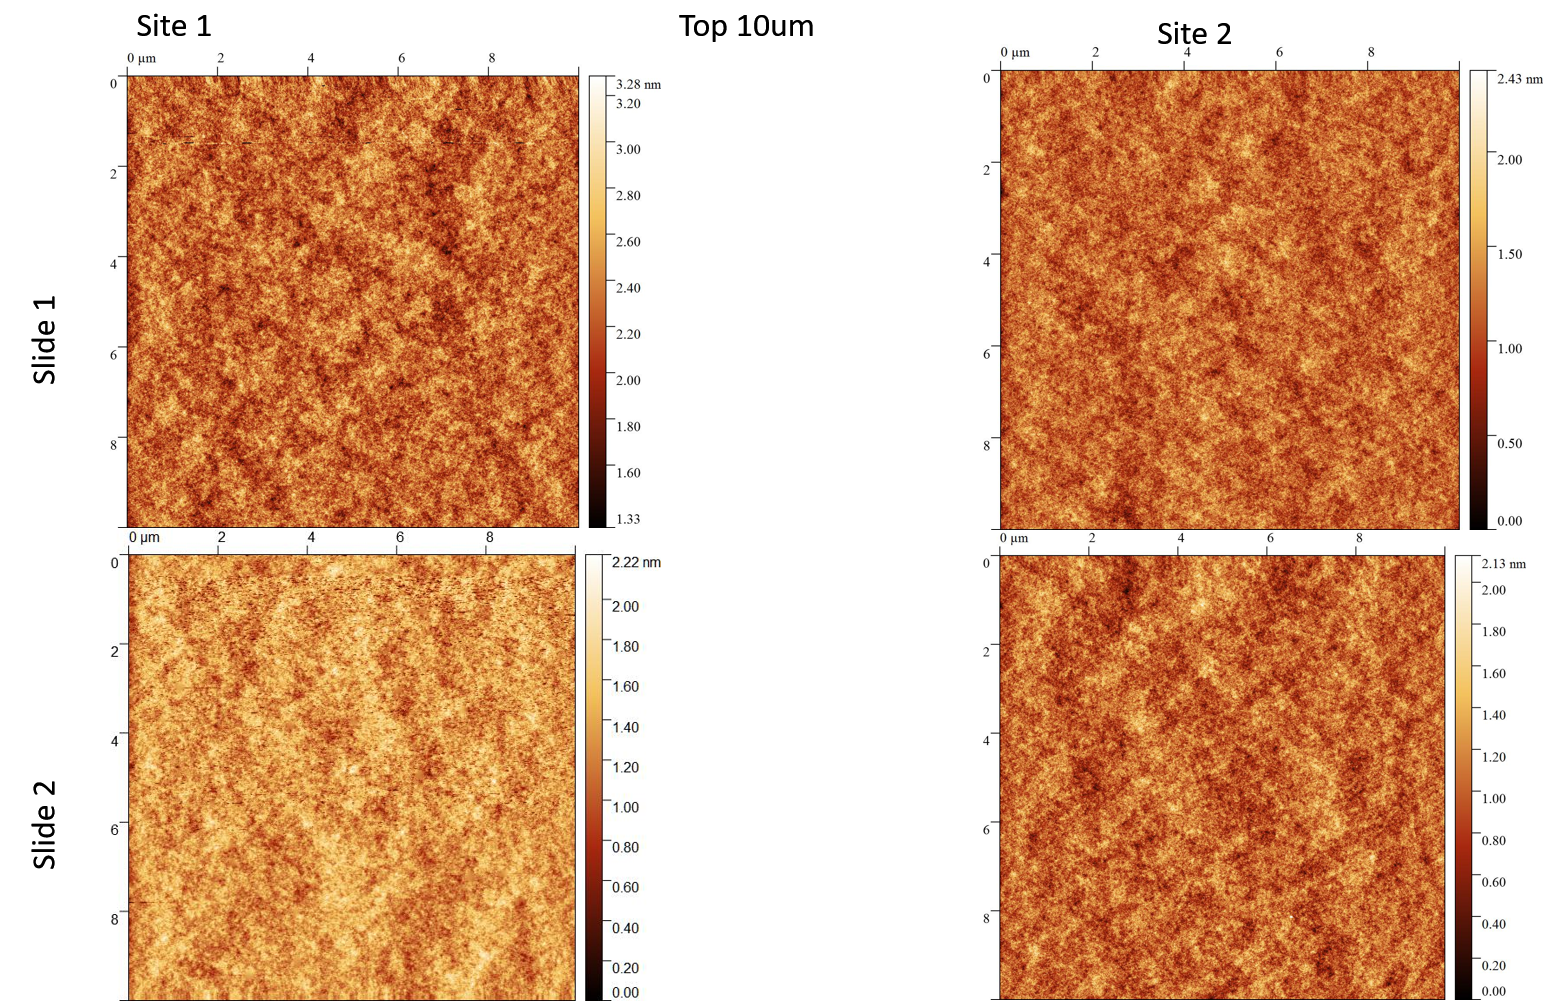
\includegraphics[width=100mm]{chapter3/Top 10um.png}
\end{center}
\caption{Four AFM images of untreated borosilicate glass on two different glass surfaces, with two sites per glass slide. The image has a scan size of 10$\mu$m x 10$\mu$m.}
\label{fig:figure9}                 % Reference label to the figure.
\end{figure}   

\begin{figure}[h!!!!]     %Insert a figure as soon as possible
        \begin{center}
          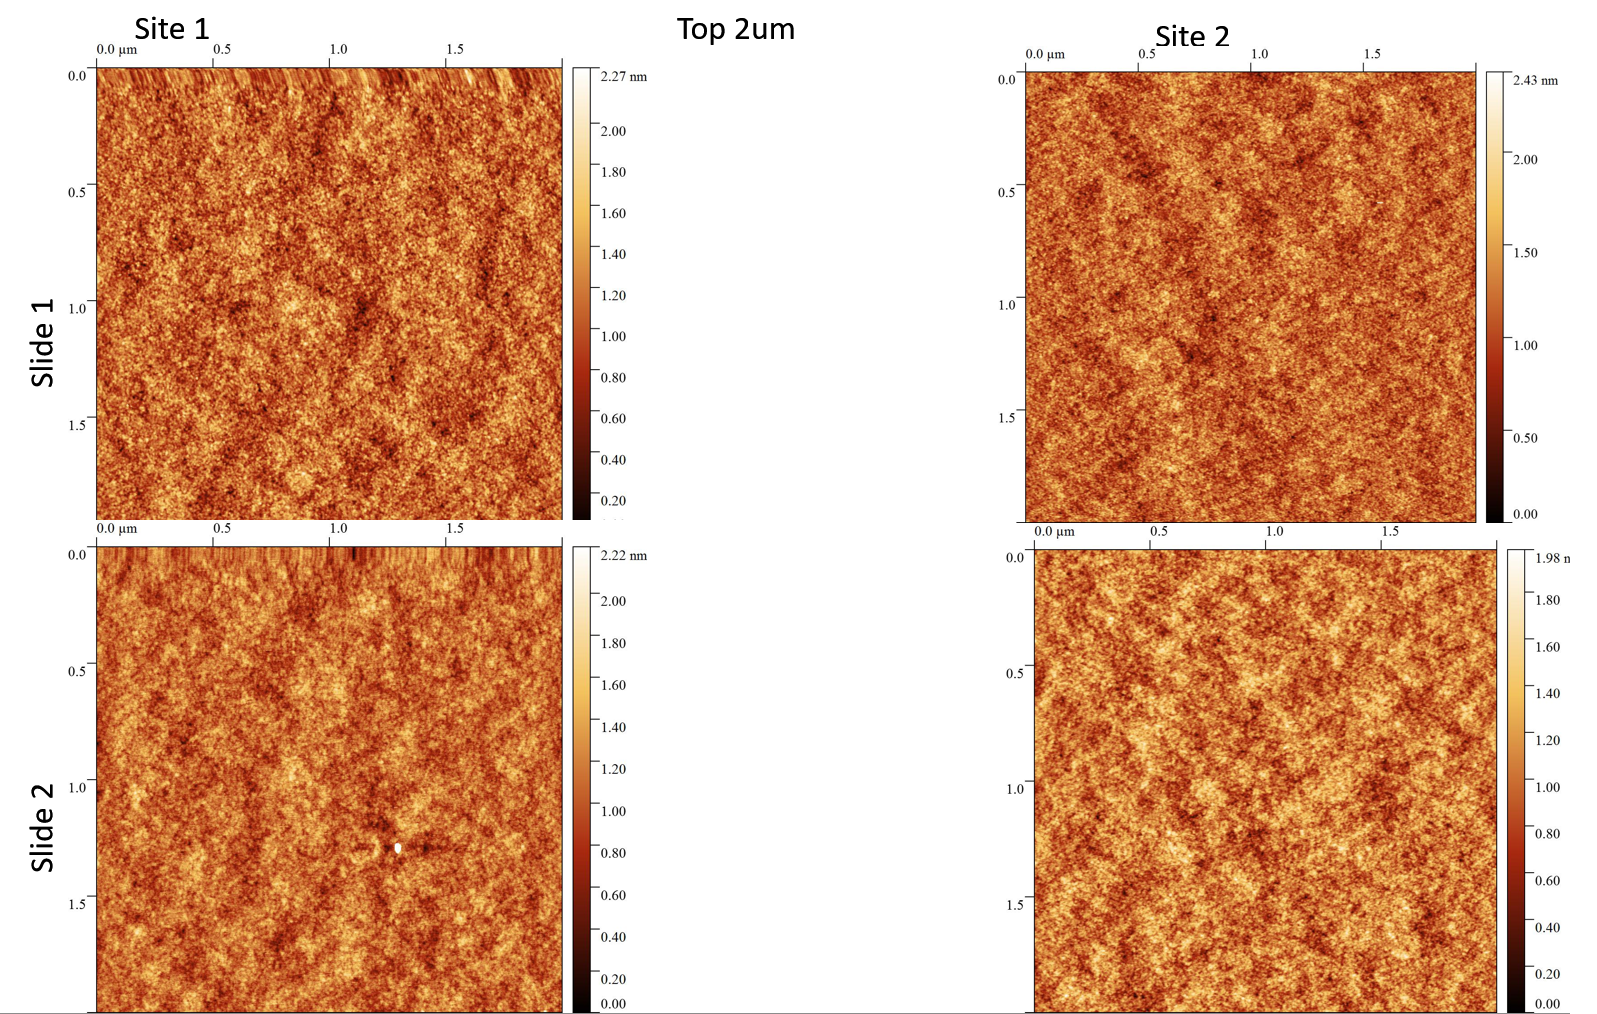
\includegraphics[width=100mm]{chapter3/Top 2um.png}
\end{center}
\caption{Four AFM images of untreated borosilicate glass on two different glass surfaces, with two sites per glass slide. The image has a scan size of 2$\mu$m x 2$\mu$m.}
\label{fig:figure9}                 % Reference label to the figure.
\end{figure}   

\newpage
The images for the middle part of the glass are shown below:

\begin{figure}[h!!!!]     %Insert a figure as soon as possible
        \begin{center}
          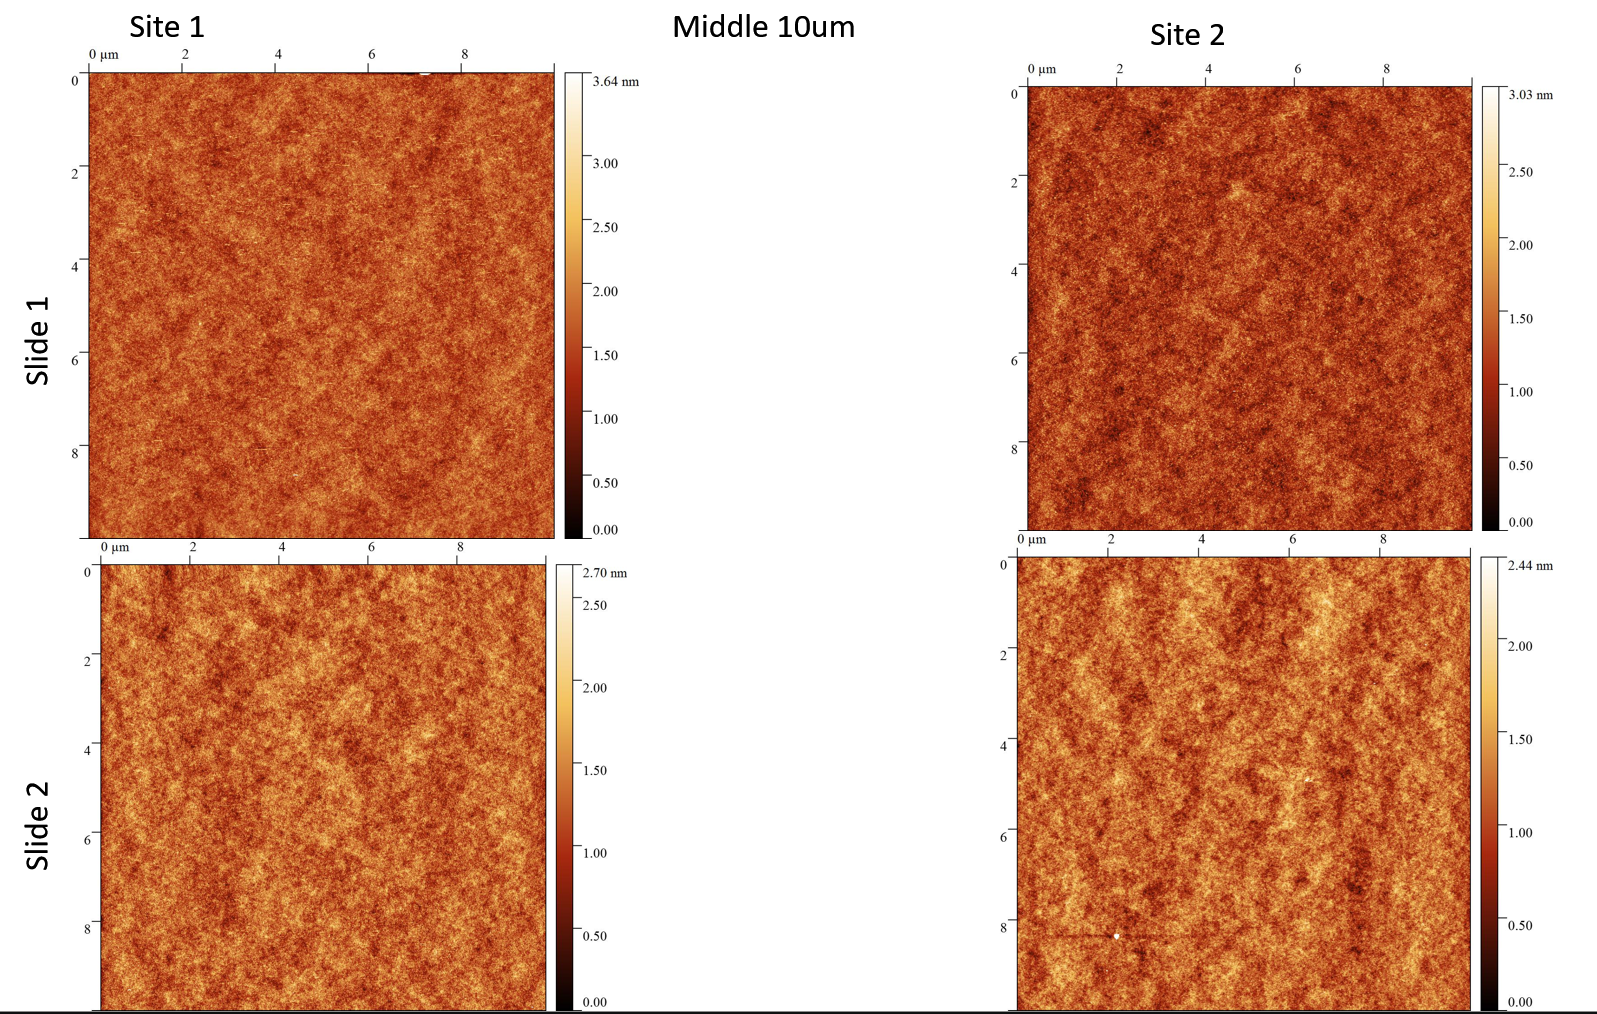
\includegraphics[width=100mm]{chapter3/mid 10um.png}
\end{center}
\caption{Four AFM images of untreated borosilicate glass on two different glass surfaces, with two sites per glass slide. The image has a scan size of 10$\mu$m x 10$\mu$m.}
\label{fig:figure9}                 % Reference label to the figure.
\end{figure}   

\begin{figure}[h!!!!]     %Insert a figure as soon as possible
        \begin{center}
          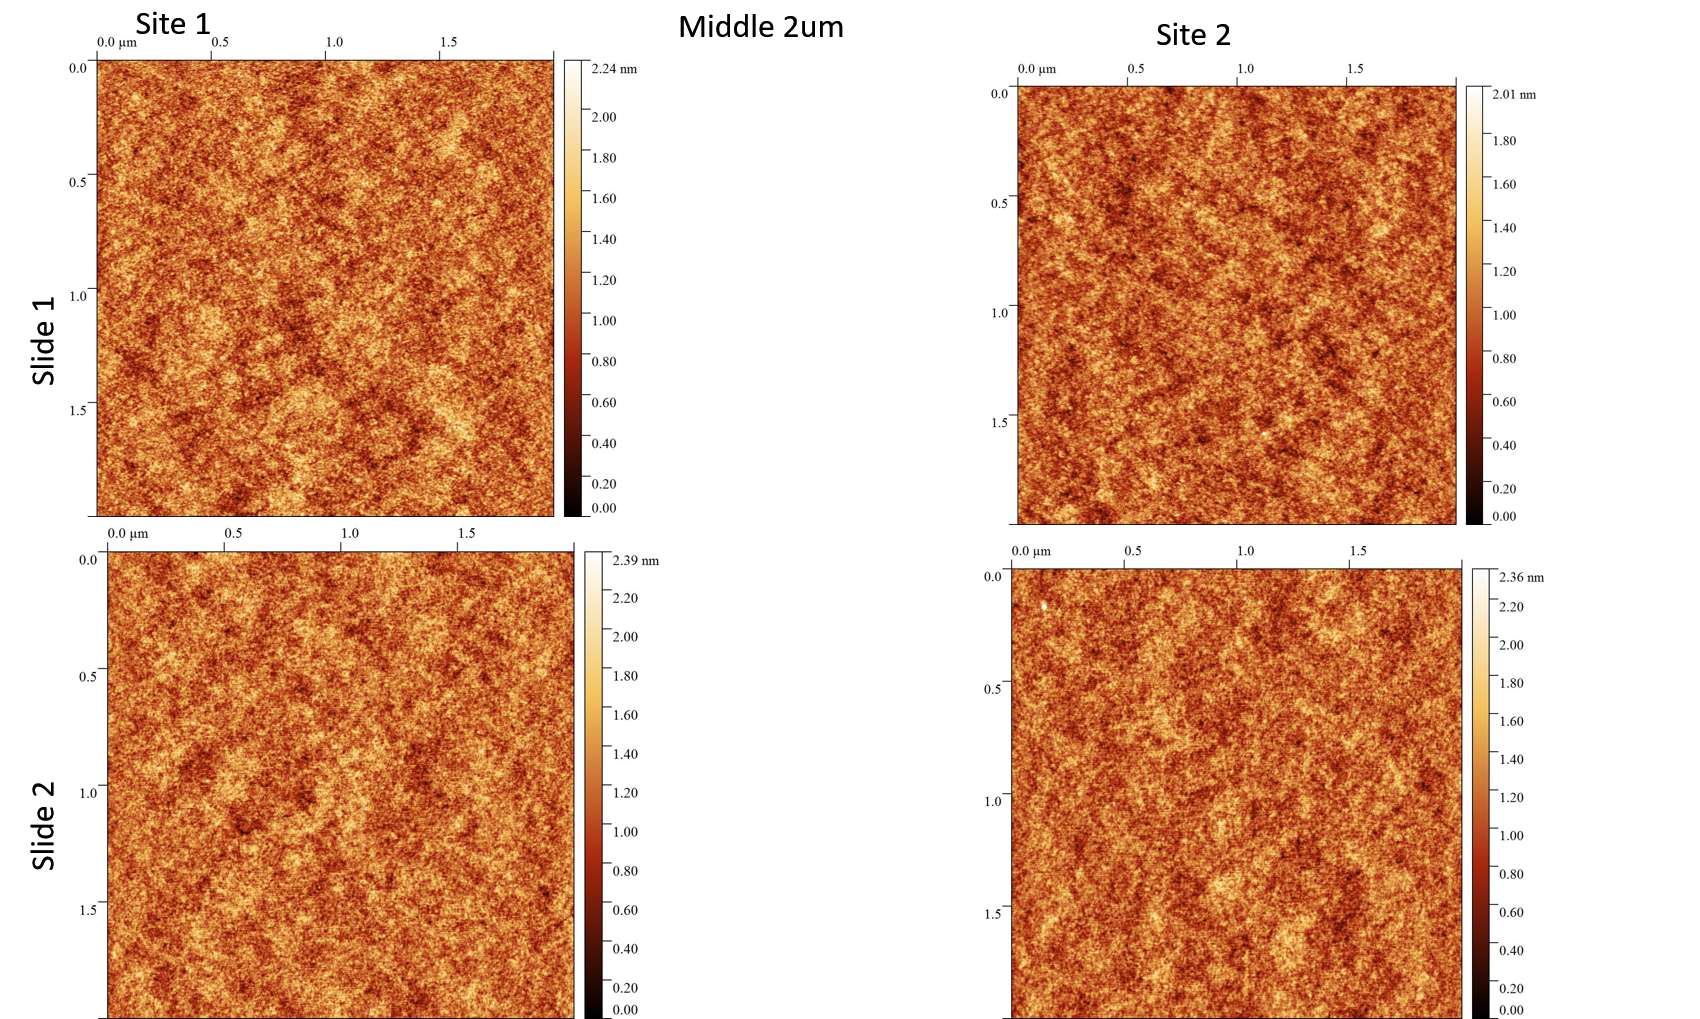
\includegraphics[width=100mm]{chapter3/mid 2um.png}
\end{center}
\caption{Four AFM images of untreated borosilicate glass on two different glass surfaces, with two sites per glass slide. The image has a scan size of 2$\mu$m x 2$\mu$m.}
\label{fig:figure9}                 % Reference label to the figure.
\end{figure}   

\newpage
The images for the bottom part of the glass are shown below:

\begin{figure}[h!!!!]     %Insert a figure as soon as possible
        \begin{center}
          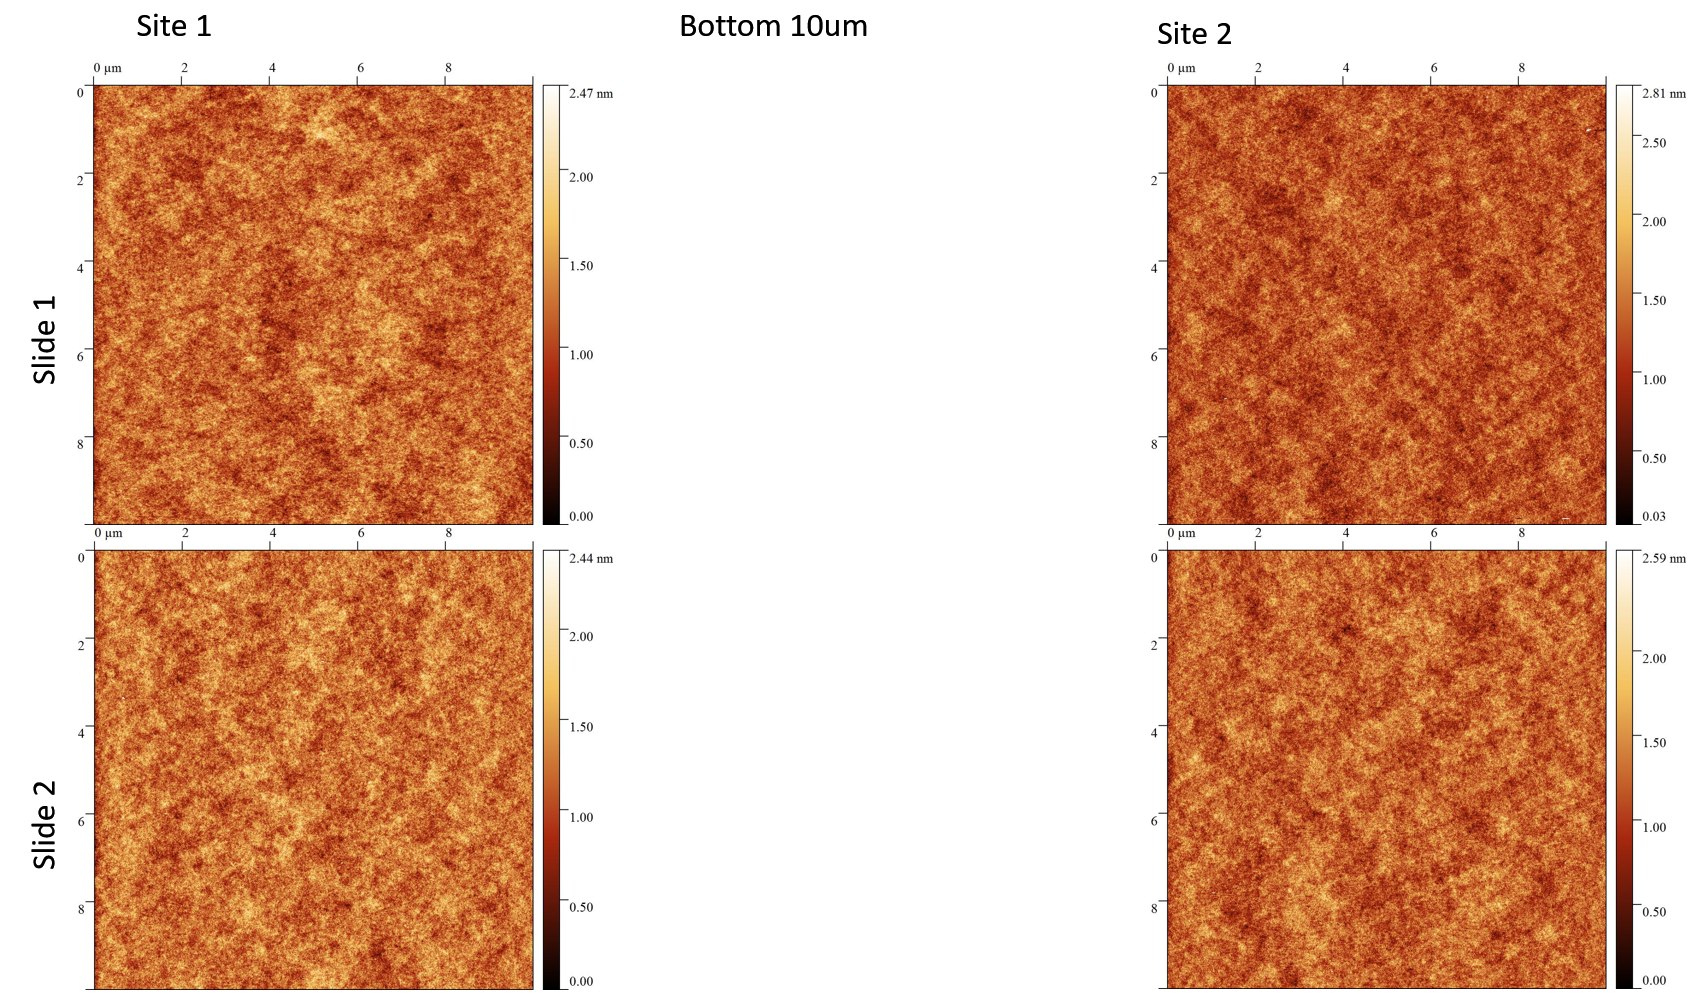
\includegraphics[width=100mm]{chapter3/bot 10um.png}
\end{center}
\caption{Four AFM images of untreated borosilicate glass on two different glass surfaces, with two sites per glass slide. The image has a scan size of 10$\mu$m x 10$\mu$m.}
\label{fig:figure9}                 % Reference label to the figure.
\end{figure}   

\begin{figure}[h!!!!]     %Insert a figure as soon as possible
        \begin{center}
          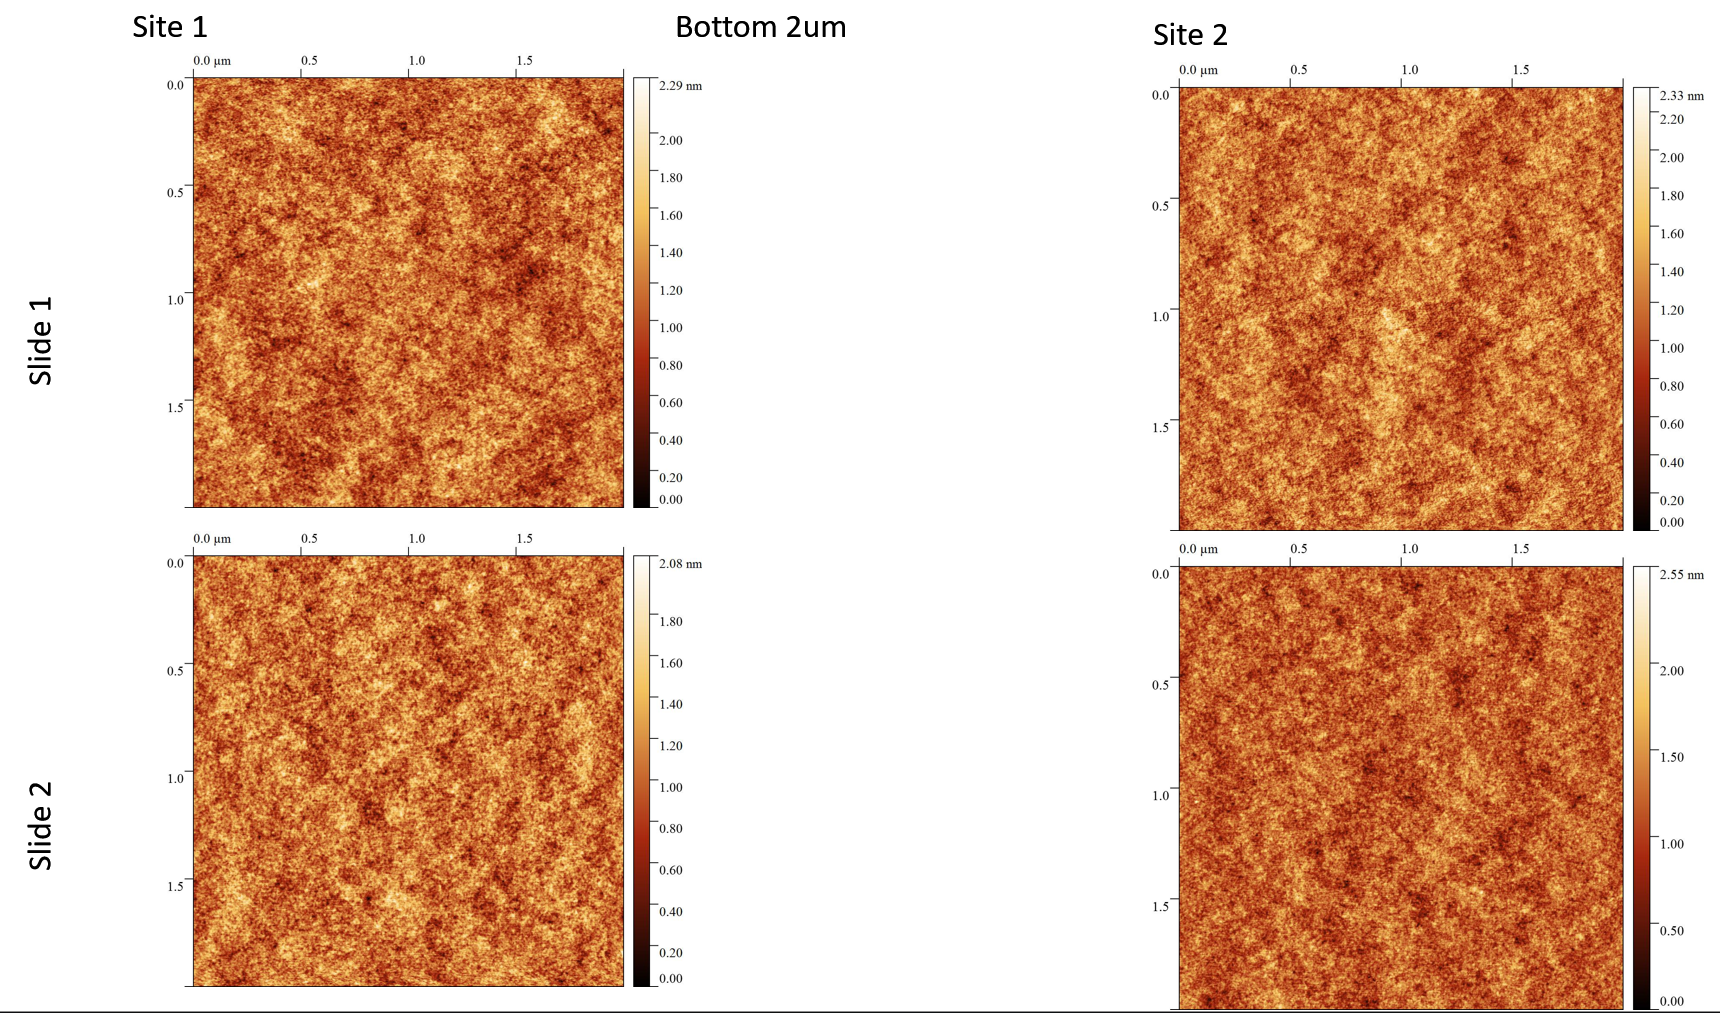
\includegraphics[width=100mm]{chapter3/bot 2um.png}
\end{center}
\caption{Four AFM images of untreated borosilicate glass on two different glass surfaces, with two sites per glass slide. The image has a scan size of 2$\mu$m x 2$\mu$m.}
\label{fig:figure9}                 % Reference label to the figure.
\end{figure}   

The AFM analysis of borosilicate glass surfaces demonstrated remarkable uniformity across the dataset of 24 images. The root mean square (RMS) roughness is a statistical measure of surface texture, calculated from the height data obtained in AFM imaging. RMS roughness is determined by taking the square root of the average of the squares of the height deviations from the mean plane of the surface within the scanned area. This gives a quantitative assessment of the surface's vertical irregularities. Additionally, peak-to-peak roughness in Gwyddion refers to the difference in height between the highest and lowest points within the scanned area, providing a direct measure of the surface's vertical variation.\cite{gwy}

Notably, the maximum peak-to-peak roughness was measured at 3.64nm for images with a scan size of 10$\mu$m x 10$\mu$m, and 2.55nm for those at 2$\mu$m x 2$\mu$m. The average root mean square (RMS) roughness values, calculated from the height variations across the scanned area, were 0.244 nm +/- 0.014nm for 10$\mu$m x 10$\mu$m images and 0.236nm +/- 0.015 nm for 2$\mu$m x 2$\mu$m images. These RMS values reflect the average height deviations from the mean plane with the standard deviation, providing a quantifiable measure of surface texture. Together the RMS was 0.240nm +/- 0.015nm. The consistency of the RMS roughness across both image sizes and sites indicates a homogenous surface texture irrespective of the scan area. Figure \ref{fig:figure9} presents representative images from each scan size category, illustrating the general surface topology observed. The consistent topology and roughness throughout the capillary's length and across multiple capillaries suggest that the surfaces used in the main investigation bear a similar structure to those depicted in Figure \ref{fig:figure9}.\cite{AFMbactPaper}
  

\subsubsection{Drift anaylsis}

In order to ensure that any error incurred by physical drift was accounted for an investigation into the x, y and z axis drift was explored. The AFM was left to image the same glass sample repeatedly in order to produce the same image several times. This image was then two dimensionally cross correlated with the next image in the sequence and the difference removed between the two z data points. The results are displayed in Figure\ref{fig:CrossCor}.

\begin{figure}[h]     %Insert a figure as soon as possible
        \begin{center}
          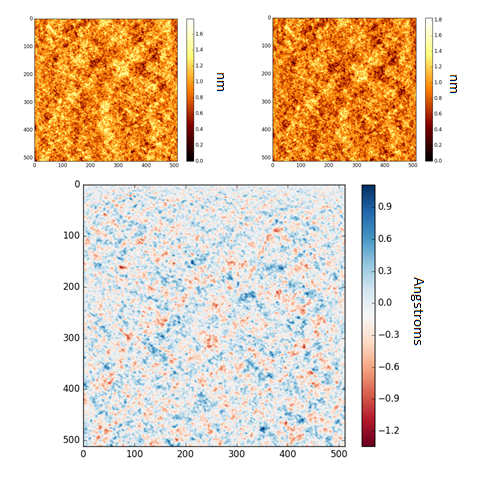
\includegraphics[width=120mm]{chapter3/CrossCor.png}
\end{center}
\caption{The output image of the 2D cross correlation function between the two images. The two smaller images are the input images into the script. The x and y values are the location of the z values in the 2D matrix dataset. The z scale is labeled respectively.}
\label{fig:CrossCor}                 % Reference label to the figure.
\end{figure}

Due to the drift experienced while scanning, the rows were found to be increasingly misaligned towards the bottom of the image. The result of this is shown by the gradient seen from the top of the image downwards , as the first image scanned from the bottom up, then the second image was scanned from the top down. The process was repeated on a row by row alignment basis and the resultant drift between the two images was found to be approximately 1 angstrom on the z axis, 8nm on the y axis and 28 on the x axis. However given the speed of the scan was low at 0.4Hz each image took approximately 40 minutes to image, giving an approximate drift of 0.1nm by 0.5nm drift per minute.

It was concluded from this analysis that the artificial effects of drift on the measured surface roughness would ultimately be negligible. Due to the small drift observed over time the influence of the resulting plane angle at points drifted towards would not have a large enough influence to impact the calculated roughness.

%Surface treatment



%\section{Glass surface cleaning}

%In order to ensure that the glass used in experiments was free of contaminants a study was performed to determine the cleanliness of the surface.



%SILICA TIP SURFACE

\section{Silica particle surface resolution} % MOVE TO CHAPTER 3 PLEASE

In order to determine the surface roughness of a silica sphere, a range of 1.5$\mu m$ silica spheres were placed upon a suitable surface and imaged. The objective was to discern any roughness variances between a flat silica surface and a spherical one. The methodology was influenced by the AFM tips used in in Chapter 4, which involved cantilevers with silica spheres attached.



\begin{figure}[h]     %Insert a figure as soon as possible
        \begin{center}
          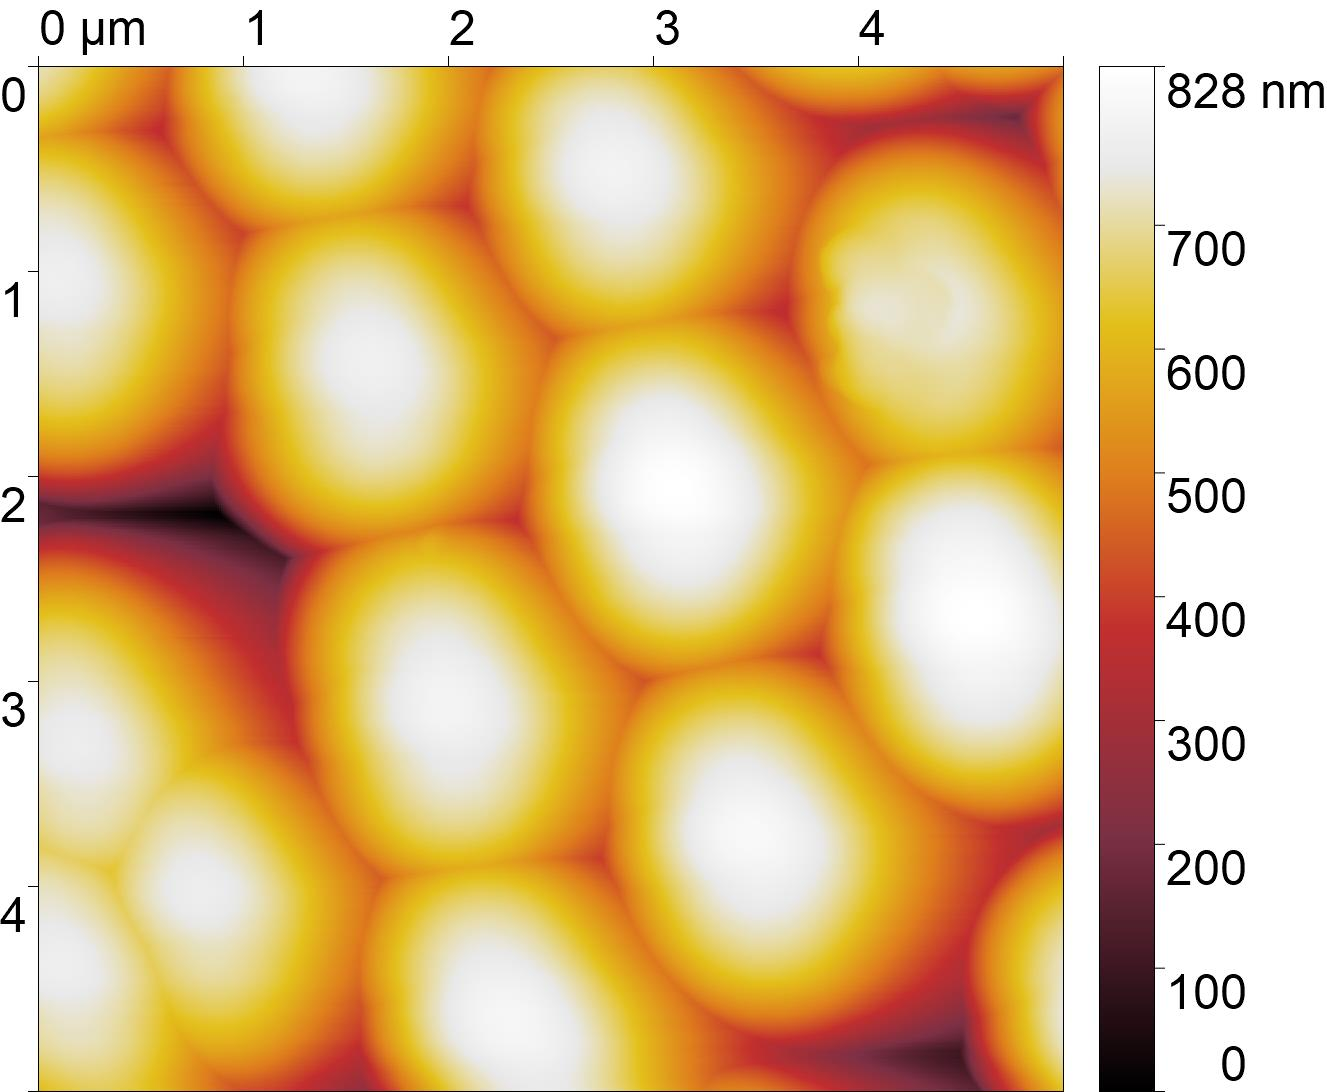
\includegraphics[width=110mm]{chapter3/5umareat2.jpg}
\end{center}
\caption{The observed surface of a silica sphere.}
\label{fig:SiliSph1}                 % Reference label to the figure.
\end{figure}

Initially, several scans were required in order to "zoom in" on an individual sphere. Due to the AFM's limit of 512 data points per line, the resolution of an individual sphere suffered unless it was the focus of the scanning frame. However, due to the drift in location due to pizeo error, attempting to suddenly zoom into a specific surface would dislocate the frame of reference from the intended area. As a result, an individual sphere was slowly zoomed in until it was the focus of the frame. This greatly reduced the range of images that could be taken and used.

Another feature of these sphere is their hexagon appearance under AFM. This is due to the tip's geometry, which limits the area it can reach, and therefore probe. As the geometry of the tip is pyramidal in shape and the true shape of the sphere is spherical, the areas that are unreachable by the probe are reported with a straight line and the height around the sphere are erroneously high. However, due to the intent of the procedure being focused on mapping the surface of a sphere, this does not affect the results as an area outside of this interference was chosen.



\begin{figure}[h]     %Insert a figure as soon as possible
        \begin{center}
          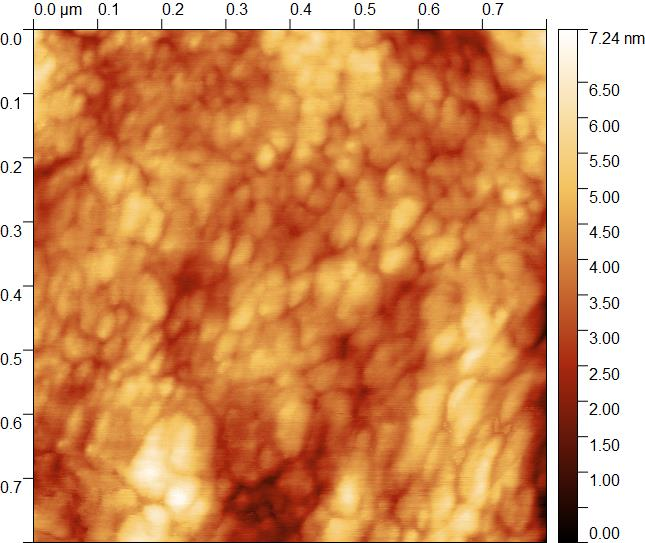
\includegraphics[width=100mm]{chapter3/Sphere3.jpg}
\end{center}
\caption{The flattened surface of a silica sphere.}
\label{fig:SiliSph2}                 % Reference label to the figure.
\end{figure}

The curvature inherent to the spherical geometry of silica beads presents a unique challenge for AFM analysis. Subsequent to imaging, any dataset inclinations or plane shifts were computationally rectified to ensure an accurate representation of the surface topology. This step was performed to remove any systematic tilt or distortion that could obscure the genuine surface features being studied. To isolate the surface characteristics accurately, advanced image processing techniques were employed. A 5th order polynomial fit was applied to \ref{fig:SiliSph1} in order to produce \ref{fig:SiliSph2}, effectively removing the curvature and normalizing the data to a flat plane. Further refinement was achieved by cropping the image, ensuring that only the relevant surface area remained within the data frame.

An AFM imaging of 3 1.5$\mu$m silica spheres was performed, and spherical deconvolution was subsequently executed using Gwyddion software \cite{gwy}. From three functional sites across different spheres, an average RMS roughness of 0.646 nm was discerned, highlighting a notable difference in roughness compared to borosilicate glass. This suggests that silica spheres exhibit a higher degree of surface roughness.

\begin{figure}[h!!!!!]     %Insert a figure as soon as possible
        \begin{center}
          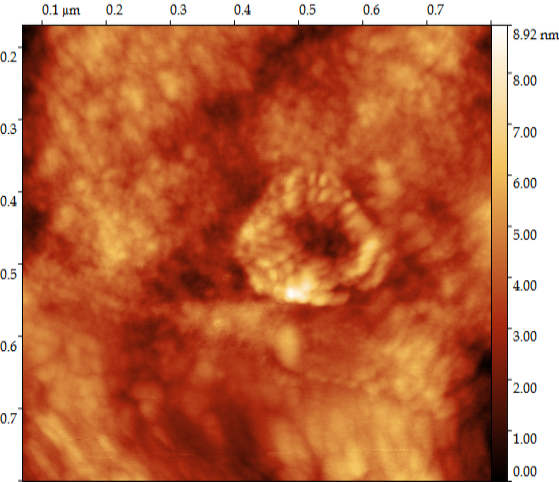
\includegraphics[width=100mm]{chapter3/Sili2.png}
\end{center}
\caption{The flattened surface of a silica sphere with a uniquely seen feature. The RMS roughness of this image was 723.5pm, the highest one in the dataset.}
\label{fig:SiliSph3}                 % Reference label to the figure.
\end{figure}

The unique feature observed in \ref{fig:SiliSph3} could originate from various sources: a surface defect, an impurity, manufacturing-induced irregularities like bubbles or pits, or possibly artifacts related to the AFM process, such as tip convolution effects. Further investigative work is suggested to understand the adhesive interactions between silica particles and to determine if the central ``pit" seen in the images is a consequence of the sonication process used to create the silica spheres. \cite{SilicaGrowth}

\newpage

%AFM force curve operation
%Done
%AFM methodology development.

%glossary nomenclature

%Have done
%Experimental setup
%AFM overview
%Script mechanics

%Todo
%Tidy MFP overview - Done
%Update Debye graph with new version - Done
%JPK overview and experimental setup - Done?
%JPK Script mechanics - Done
%Use example graphs to plot the narrative though a single example case for bin size

\chapter{Atomic force spectroscopy analysis}

\section{Introduction}

This chapter explains the experimental methods used for force curve collection as well as the computational methods used to interpret them. Over the course of data collection the process was refined to a repeatable method across a consistent experimental setup. While two different AFMs were used across the analysis, encouraged by technical limitations, they were used in such a way to complement one another. Both of these AFMs were used to produce force curves, and were interpreted using the same scripts.

\section{MFP-1D} %possibly put this first 

\begin{figure}[h!]     
        \begin{center}
          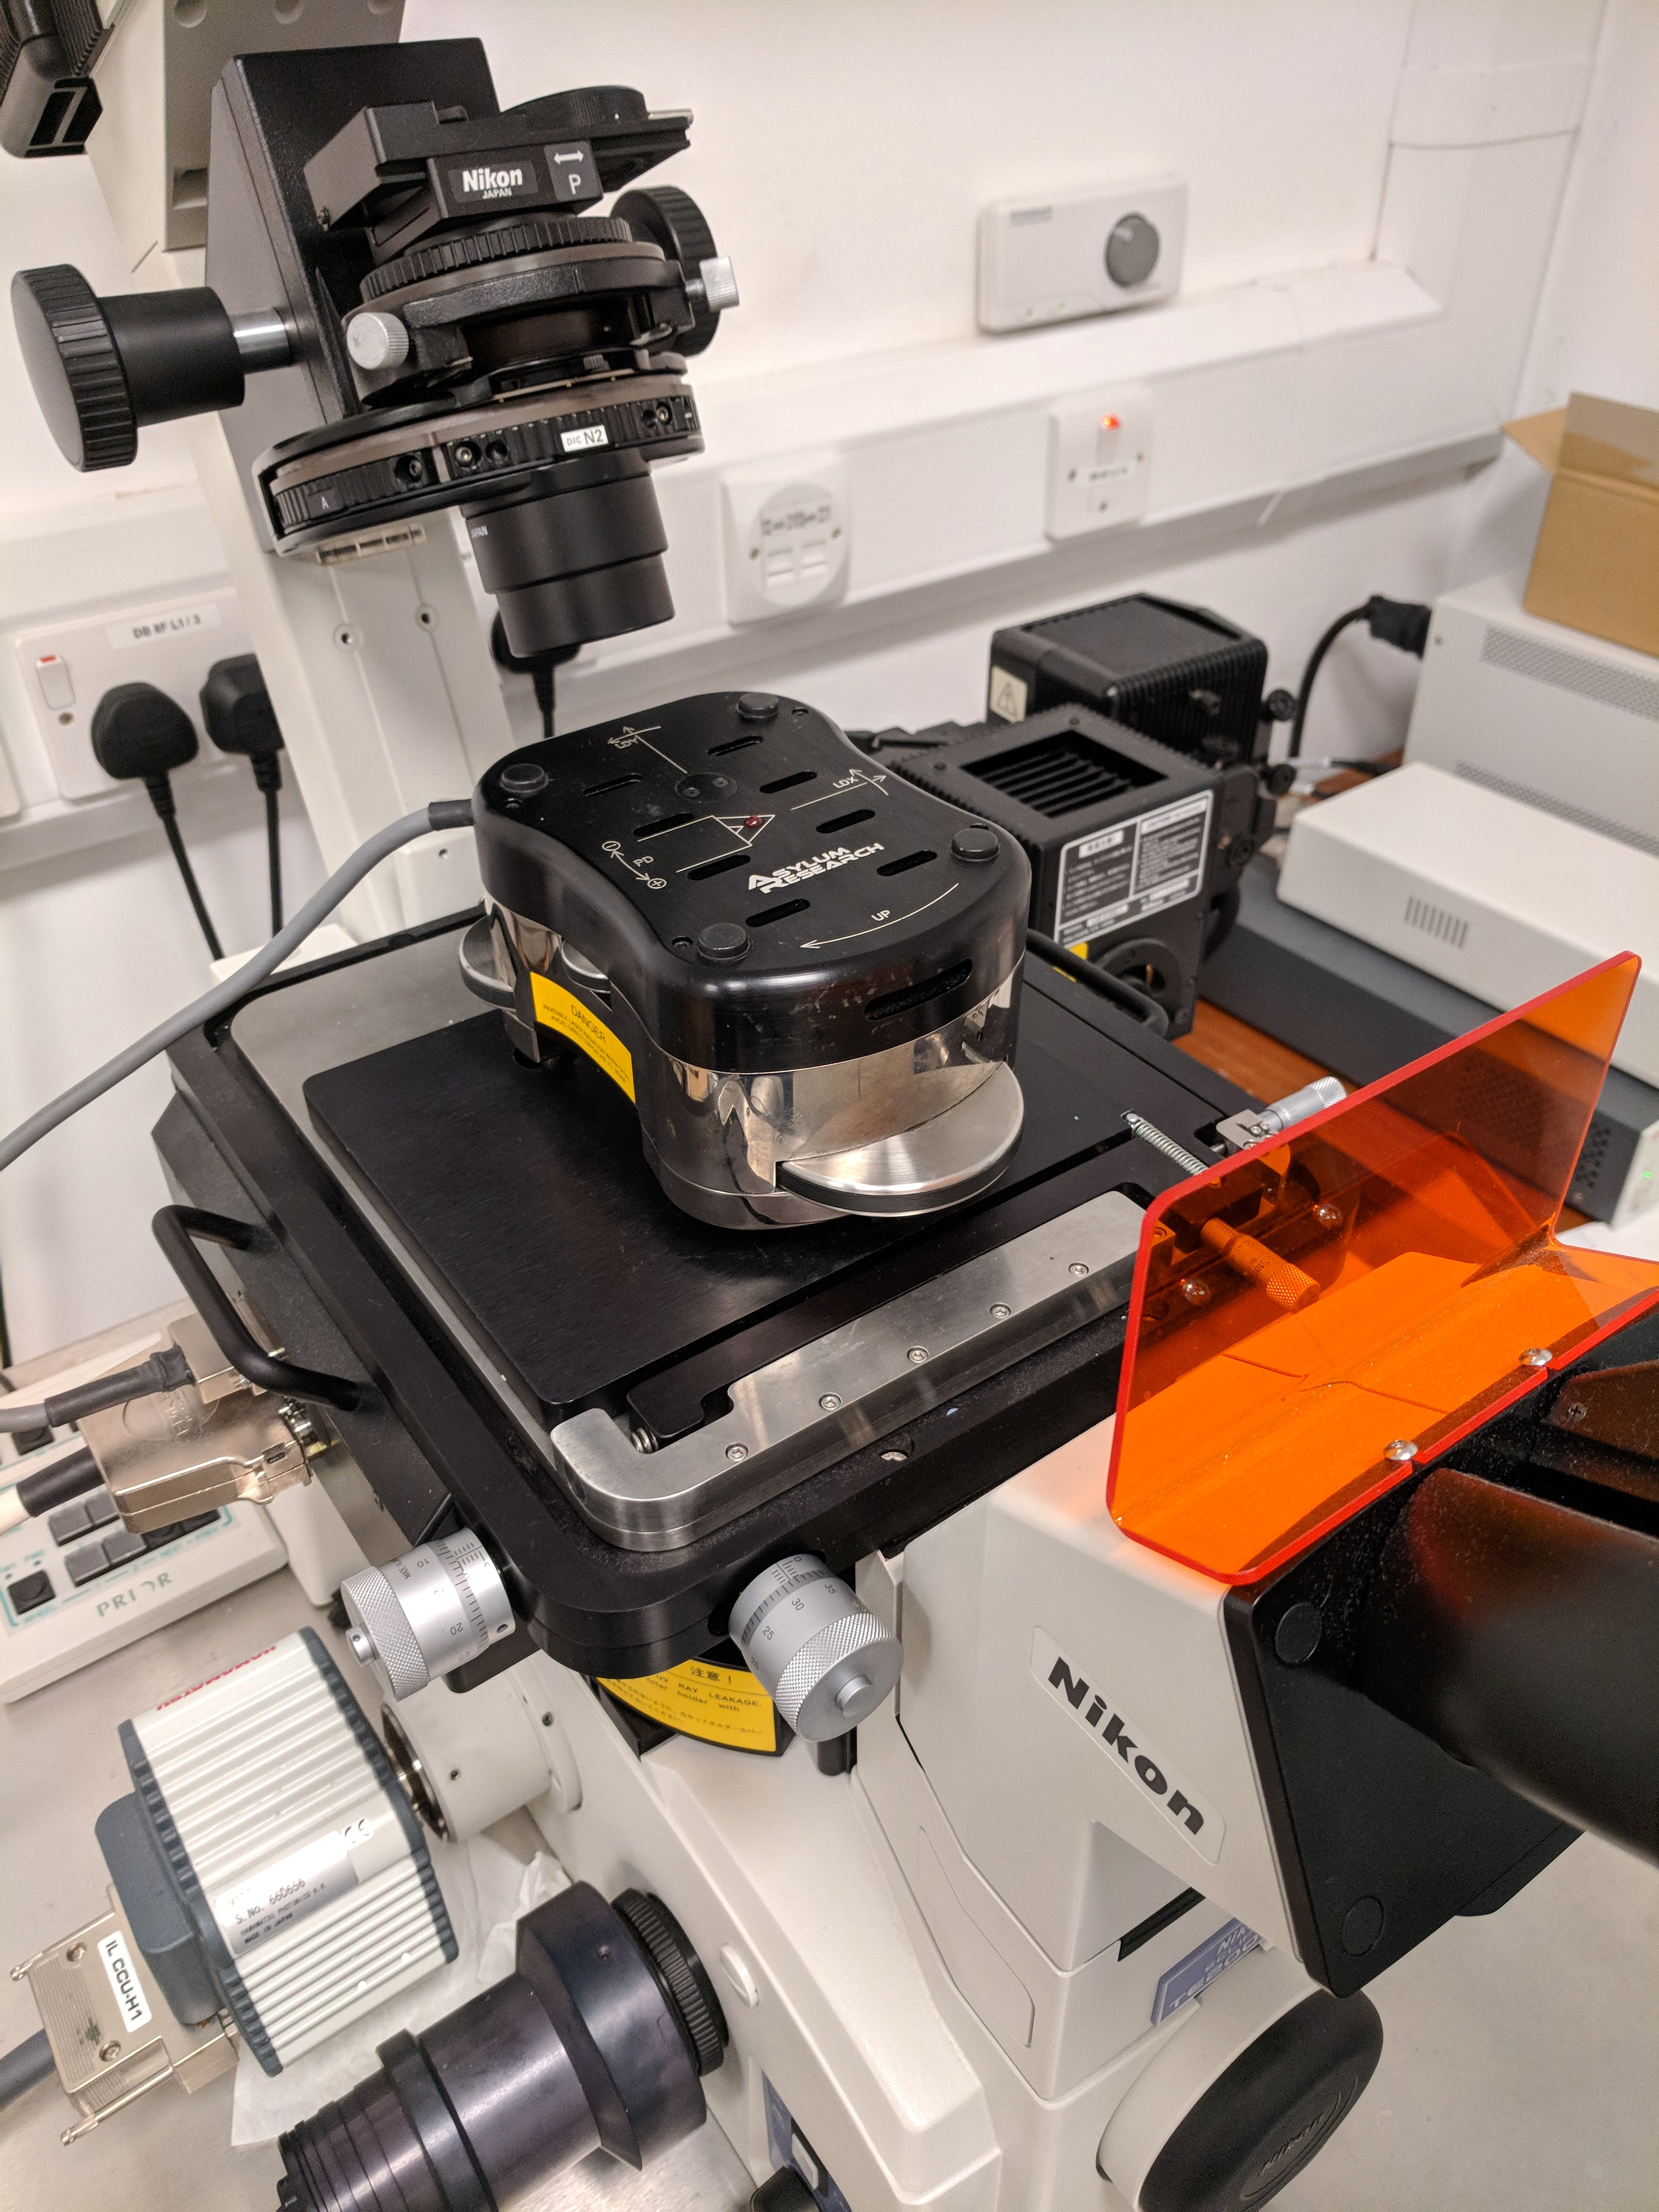
\includegraphics[width=80mm]{chapter2/forceAFM.jpg}
\end{center}
\caption{Operation setup for the MFP-1D AFM that was used for force measurements.}
\label{fig:forceAFM.jpg}                 
\end{figure}

For the force spectroscopy setup a MFP-1D from Asylum Research was used. The MFP-1D is an AFM mounted on top of an inverted light microscope, with the sample placed between the scanning head and the stage of the light microscope. In the AFM head the cantilever is mounted using tweezers in a holding apparatus. This head is immobile in the X,Y direction, horizontal movement is instead controlled by manlipulation of the stage. In the Z direction there are two possible movements - the 3 legs of the head can be moved vertically using the wheels for coarse movement, either to bring the tip in contact with the sample, or to level the head so the contact of the tip with the surface is uniform. The other control over the vertical height is via the piezoelectric transducer (piezo) mounted in the center of the head. This piezo has a travel range of roughly \SI{15}{\micro\metre}. A laser is then emitted from inside the head and directed onto the cantlever, towards the sample. (See fig ~\ref{fig:Head.jpg})

For laser alignment on the AFM head an inverted microscope is used. First the cantilever is brought into focus under the microscope, then the position of the laser is aligned atop of the intended cantilever. Afterwards the laser is focused upon the center of the tip using the sum output given by the photosensitive diode. The diode converts incident light into an output voltage, this allows the position of the laser focal point to be determined with respect to the diode boundaries.  Finally the deflection of the laser is set to 0; a central position between the positive and negative extremes. Deviation of the laser's focal point from the center point of the photodiode allows movements of the cantilever to be detected. This detects any bending (and thus attraction/repulsion) of the cantilever. 

In terms of the structure of the device, it differs slightly to the imaging AFM explained in the previous chapter; the components are more tightly packed, mounted atop of the z-piezo directly, which then brings the apparatus down onto the sample, unlike the z-piezo raising the sample up to be imaged. In addition a linear variable differential transformer (LVDT) sensor is mounted inside of the head to correct the movement of the z-piezo (closed-loop piezo) thus improving z-piezo accuracy (See fig \ref{fig:Head.jpg}).

\begin{figure}[h!]     %Insert a figure as soon as possible
        \begin{center}
          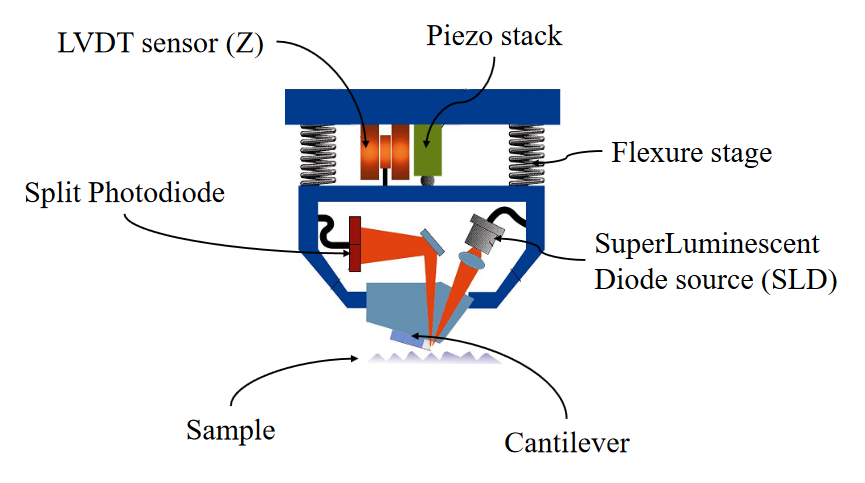
\includegraphics[width=80mm]{chapter2/Head.PNG}
\end{center}
\caption{Operational setup for the MFP-1D AFM that was used for force measurements. Adapted from \cite{AFMTalk}} %remake in jost style to reduce concerns
\label{fig:Head.jpg}                 % Reference label to the figure.
\end{figure}

%Add how vibrations in the building resolve into experimental noise and therefore dupe the system into thinking it's hit the surface.

Due to this feedback loop from the LVDT relying on previous data to define the voltage control from the next approach, the peak force (the intended maximum force applied on the cantilever per curve) was set to a relatively low number 8 nN. This was done to limit the amount of tip damage during operation. In cases where the tip fails to engage with the surface in the previous approach, this low peak force ensured re-engagement of the tip with the surface in the current loop was as gentle as possible. Noise in the data was attributable to the effect of vibrations on the operation of the instrument. When errant vibrations reach the AFM, this energy is transferred through to the cantilever, which then causes it to oscillate. This oscillation usually presents itself as a sudden spike in deflection on the curve. It is these sorts of curves that are selected and removed from the dataset. In most cases the total amount of removed curves is minimal, usually 1 or 2 per site, with a total of 100 or more curves used for processing. While it was rare that any datasets were rejected for purely noise based reasons, there is one notable set that was repeated at a later date due to a storm causing significant, persistent errors in the data. While the AFM was mounted on an anti-vibration table, the noise observed in the machine is still present.

Additionally, the standard speed of tip movement was set to \SI{1}{\micro\metre/s} (unless otherwise stated). This was done to compromise between the total dataset recording time and reduction of strain upon the cantilever and tip.

\subsection{Experimental setup}

\begin{figure}[h!]     %Insert a figure as soon as possible
        \begin{center}
          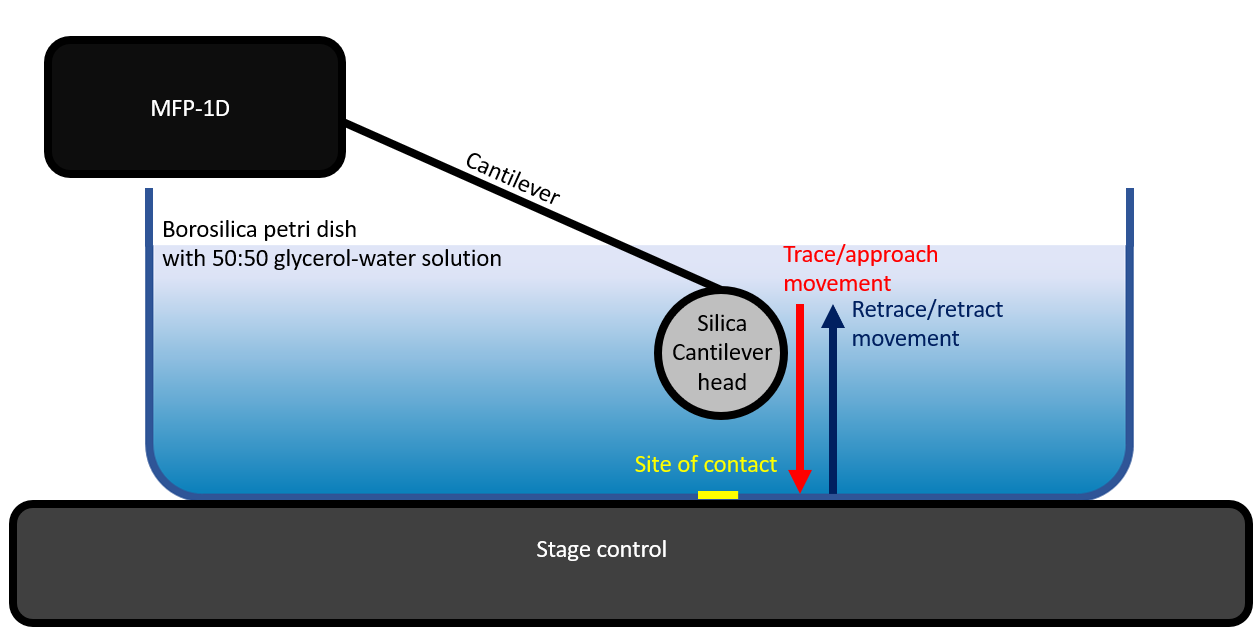
\includegraphics[width=110mm]{chapter4/Chapter4ExperiSetup2.PNG}
\end{center}
\caption{Experimental schematic of MFP-1D during operation. The AFM is abstracted away into a back box to highlight the motion that the cantilever takes with respect to the surface. The stage control provides horizontal control, and therefore moves the projected site of contact along the petri dish surface.} 
\label{fig:Chapter4ExperiSetup}                 % Reference label to the figure.
\end{figure}

%Diagram of interaction!!!!

\subsubsection{Initial Setup and Challenges}

Initially the experimental setup was focused on investigating the interactions between two silica particles. Given the difficulty in aligning two micron sized particles for interaction, the geometry of a silica particle and a flat silica surface was chosen. In order to facilitate this approach a silica particle was glued to a cantilever (see fig \ref{fig:Chapter4ExperiSetup}). These types of cantilevers are produced commercially, with the gluing process as part of the manufacturing, and were purchased to reduce experimental setup time. This cantilever was then brought into contact with a silica surface, with the results transformed using the Derjaguin approximation (See chapter 1). 

The first setup involved a \SI{1.6}{\micro\metre} diameter tip brought into contact with a silica surface glued to the inside of a plastic petri dish. This setup allowed for a liquid solution to be placed on top of the surface, contained within the plastic petri dish. A 50:50 (by volume) solution of deionised water and glycerol with a controlled concentration of LiCl was added. This ratio was chosen by volume to ensure consistent mixing and ease of preparation, given the liquid nature of both components. Glycerol was chosen for its high viscosity and low volatility, which help stabilize the solution during AFM measurements by reducing evaporation and maintaining a consistent environment for the silica particles. The increased viscosity allows for more controlled measurements of the forces between particles, providing insights into how these forces scale from single-particle interactions to multi-particle interactions within a viscous medium. This solution was brought up to completely cover the tip, ensuring the head of the AFM was submerged.

The initial setup involved calibrating the cantilever tip on a separate calibration surface (see chapter 2), then removing this surface and replacing it with the experimental one. Initially approaching the glass surface in air was of little issue, but the greatest difficulty arose in finding contact with the glass surface under liquid. Given that the liquid in use was of similar optical density to glass, the interface between the two was no longer visible under the microscope. As a result; the initial approach was slow, methodical and careful, as recklessness would break the tip. 

\subsubsection{Issues Identified and Interim Solutions}

Problems with the setup were identified after a test run, after a sweep of 4 different concentrations it was found that the resulting Debye lengths for all the curves were above 6 nm. These were directly contrary to the expectation that Debye length should decrease to theoretically 0 at increasing salt concentrations. The anomalous readings were considered to be the result of unidentified contaminants. Given the setup with the AFM was open by necessity as well as the difficulty in getting the sample under the tip in an expedient manner, there was little protection against airborne contaminants. Additionally, contaminants originating from the the plastic of the petri dish and glue were identified as a source of problems. The method of cleaning the surface was also called into question. %considering rewriting for flow
%EXPECT A VIVA QUESTION HERE!

In order to address these issues, a few changes were implemented over a series of experiments. The surface used was exposed to an improved washing protocol. This washing protocol used deionised water to clean the surface over a greater period of time. Ethanol was considered, but due to the glue holding the surface down, there were concerns over the surface having a stable platform. Additionally the method of approach was revised slightly, with a large part of the distance between the surface and the tip performed in air, with the liquid solution injected using a glass pipette slowly. This injection relied on the surface tension of the water to slowly fill the dish, resulting in a slightly higher volume use. This was done to minimize any dramatic flow from damaging the tip, emulating a normal approach submerging mechanics. %Finally any glass wear use was limited to one use only instead of attempting to clean. - I mean that's kind of standard in anything, worth mentioning?
%VIVA QUESTION POTENTIAL

Contamination issues were still present after these revisions. In order to maximise contaminant removal, the plastic petri dish was replaced with a borosilicate glass one. Instead of gluing a surface on top of the petri dish, the surface of the dish itself became the sampled area. While there had been previous considerations of the stability of the glue influencing the resulting force curve, the approach had been focused on solving the contaminant problem first. By using the surface of the dish itself, any concerns regarding glue induced artifacts could be laid to rest. This new dish permitted the use of ethanol in the cleaning procedure, as well as plasma treatment of the surface. The silica bead diameter on the cantilever was also increased to \SI{6.6}{\micro\metre} to increase the area of contact. 

Plasma cleaning was performed under a vacuum within a sealed chamber. After the chamber was evacuated a low quantity of pure oxygen gas is flowed across the surface at 0.4 bar, with the vacuum pump still active. This plasma cleaning technique cleans off any residual organic matter, resulting in water and carbon dioxide by-products. These byproducts are pumped away by the constant vacuum. \cite{PlasUV} \cite{PlasTreat} \cite{SilicaAFMCleaning}

%At this point the strong electric fields rip electrons out from the oxygen gas, forming plasma in the surrounding area. This plasma then lets off ultraviolet light, which breaks the organic bonds present on any surface contaminants. Additionally the energetic oxygen species bind to these broken bonds, resulting in water and carbon dioxide byproducts. These byproducts are pumped away by the constant vacuum. \cite{PlasUV} \cite{PlasTreat} \cite{SilicaAFMCleaning}
%(Actual values are in 2nd lab book, will be corrected after quarantine)
%Ensure this is correct

\subsubsection{Final Protocol}

In response to the ongoing contamination problems, a final protocol was established to ensure the integrity and reliability of the experimental results. The plastic petri dish was replaced with a borosilicate glass dish. Rather than gluing a surface on top of the petri dish, the surface of the dish itself was used as the sampled area. This change removed concerns related to glue-induced artifacts and facilitated a more thorough, efficient and effective cleaning method.

The glass petri dish and lid were cleaned with ethanol and water, then followed by plasma treatment. The plasma cleaning process was conducted under a vacuum within a sealed chamber, with a controlled flow of pure oxygen gas at 0.4 bar. This procedure  removed residual organic matter, further minimizing potential sources of contamination.

During the AFM setup and operation, the cantilever was carefully mounted into the AFM head, and the laser was aligned as precisely as possible to the center of the photodiode. The petri dish was then placed under the AFM head, and its surface was utilized to calibrate and calculate the spring constant of the cantilever. Following this, the cantilever was retracted by a known amount, and the liquid solution was pipetted in. After the liquid had settled, the laser was recentered to account for the change in optical density, and the tip was brought into contact with the utmost care,  relying on deflection readouts due to limited visibility. When contact was established, between 100 and 200 curves were collected for each site. In cases where multiple sites were sampled, the tip was slowly retracted, the dish was repositioned, and the approach phase was repeated to ensure consistency.

When transitioning between different electrolyte concentrations, to manage contaminants and maintain tip reusability, the tip was retracted, cleaned with water, and plasma-treated along with the petri dish. Each tip was plasma-treated no more than twice to prevent excessive damage done to the tip from the procedure (see fig \ref{fig:ScorchedEarth}). For fresh tips, they were used as supplied from the manufacturer. Direct imagining of the petri dish was not possible due to incompatible geometry at the time of collection. 
\begin{figure}[h!]    
        \begin{center}
          \includegraphics[width=90mm]{chapter4/ScorchedEarth.png}
\end{center}
\caption{The view of a damaged chip from sequential plasma treatment. Normally a clean chip presents an observed silver colour on the outside, but from over-treatment the surface has worn away, resulting in the presentation seen above.}
\label{fig:ScorchedEarth}                 
\end{figure}

\subsection{Connection with Rheology}

The choice of experimental setup, particularly the use of glycerol and the attention to contaminant control, is essential not only for the accuracy of force measurements but also for drawing connections to rheology. The increased viscosity of the glycerol solution simulates environments similar to those found in industrial or biological systems, where the rheological properties of colloidal suspensions significantly influence their behavior under shear forces. Understanding the transition from single-particle interaction forces to multi-particle interactions in these systems can provide valuable insights into the design and optimization of products and processes that rely on controlled rheology, such as in pharmaceuticals, food science, and materials engineering.

The results from this setup are intended to bridge the gap between microscopic forces and macroscopic rheological properties, demonstrating how the behavior of individual particles can scale up to influence the bulk properties of a suspension. This connection is vital for applying the findings of this study to real-world systems, where controlling rheology is key to achieving desired product performance.
%47.2 - glycerol
%


%Majority of the data collected to be around the inflection point -
%This was done to apply as little operational damage onto the cantilever. - Mention it again earlier, but less focus on the data output side.
%Mention the time factor - 0.5Hz 2s per curve. Earlier, with the experimental setup of the AFM
%Discuss in more detail about how the curve is taken though put it in chapter 2 !!
%fluctuations in the system cause the AFM to "lose" track of the surface and therefore increase the voltage input into the movement, over-correcting it's movement, shifting the captured area further up. After this the error correction it reduces the voltage until it stabilises.
%Hurricane Leslie ruining data due to location in the building.

\subsection{MFP-1D force-distance curves acquisition and processing}

\subsubsection{Acquisition}

A minimum of 100 force curve readings per site was taken for each measurement site, with the raw data saved in a single file. The columns alternated with the raw deflection reading for one curve, followed by the corresponding z-piezo value. The majority of readings measured both the approach and retract in one single motion, combining both these curves into one whole column. In the case where the cantilever was held at a certain location for a period of time, a new set of columns is appended, with another one starting after it begins movement again, thus fracturing the data whenever the cantilever is stationary between periods.

From this each curve was broken down into two lists of raw unprocessed data given by the machine; the piezo height and the deflection. The piezo height is the recorded height of the end of the piezo (where the cantilever is mounted on) on a scale of \SI{0}{\micro\metre} to \SI{15}{\micro\metre}. This range corresponds to the effective movement of the base of the cantilever in the z direction, and is thus variable between datasets, as contact can be anywhere within this range. For example, if the pizeo moves the cantilever down by \SI{5}{\micro\metre}, and then comes into contact with the surface at that area, the recorded value will be \SI{5}{\micro\metre}, not \SI{0}{\micro\metre}. It is worth noting that the z height controlled by the legs of the AFM is independent, and is not measured by the machine. Contact is a combination of the leg height being set by the operator manually, and the piezo coming into contact within its \SI{15}{\micro\metre} range. The cantilever deflection is the deviation in nm from the equilibrium position, which corresponds approximately to the center of the photodiode. No deflection (i.e. no force) is associated (by appropriate alignment) with the laser beam hitting the centre of the photosensitive two-segment diode (corresponding to 0 Volts). Deviation from the center arises from when the cantilever is bent in a certain direction,  reflecting laser off the top of the cantilever to drift along the photodiode's sensory range. This voltage is recorded as either a positive or negative voltage corresponding to upwards or downwards deflection due to repulsive or attractive forces, respectively.  This deflection is saved alongside the height in individual data files during operation automatically, with any derivative graphs following the same naming convention defined by the input file, with respect to the unpacked raw curves. 

In some cases the resultant curve is not typical. This can arise when the cantilever doesn't move far enough down to find the surface, or when the cantilever starts in contact with the surface at the start of the movement. While these curves were rare, they did occur during standard use of the AFM. These curves were removed during processing. These erroneous movements were usually corrected automatically by the AFM via error correction feedback for the successive curves afterwards. In some cases, due to imperfections of the control mechanism of the AFM, tremors/ vibrations in the building or other uncontrollable factors the frame of reference can shift up, resulting in an unusable curve, simply due to the lack of a data in a specific area. These fluctuations in the system cause the AFM to ``lose'' track of the surface and command an increase to the voltage sent to the piezo, over-correcting its movement, shifting the captured area further up. After this the error correction the peizo controller reduces the control voltage until it stabilises around the maximum force specified by the operator. In addition, in the case of an uncontrollable error (primarily vibration based) the noise of a specific curve can throw off the normal processing of the script. It is in these instances that these curves are identified and removed.

Using Python\cite{python}, an automated script was constructed to process the large volume of data generated by the MFP-1D AFM, given that each site generated around 100-200 approach and retract curves, and that multiple sites were used for each concentration, this produced a sizeable volume of data of around 6,000 curves which would be unmanageable without some form of automation.

%Overly fluffy
%A bit word salad-y too

%Make it less about the data
%appendix

%parameters:
%cfit_min
%cfit_max
%dfit_win
%dfit_off

%Rough script overview:
%Kc is calculated during AFM operation which is then added into the script by hand.

%Creation of output directory first, mfp.split_curves
%Then reads the csv if present, otherwise generates raw data files using
%mfp.comp_def_deriv
%mfp.proc_force_sep


%Afterwards plots the separation graphs with mfp.plot_force_sep_res
%Finally calculates contact forces with mfp.get_contact_forces

%mfp.split_curves
%Creates directories:
%force curves (master folder)
%raw force curves:
%- (force (N) / z piezo position (m)) %I.e. where the pizeo is in the range of it's movement (max 5um)
%Approach (see later)
%Retract (see later)

%(also removes velocity wave curves as there is only one taken at the start (and it's not always there for random reasons, but probably don't mention that)

\subsubsection{Processing}

Using numpy\cite{numpy} an array was created from the data present in the raw data file for a specific site. Each of the curves for a given site was then split up into individual numpy arrays in preparation for the following functions. As it stands, this raw data requires at the bare minimum translation from a deflection vs distance graph into a force vs distance graph. This corresponding graph of force (nN) vs z-piezo position ($\mu$m) was produced. The raw deflection was converted into force using the spring constant of the cantilever with the following equation:\cite{KcConst}. %find citation
%VIVA QUESTION - NUMPY

\begin{equation}
F = K_c(\delta - \delta _{offset})
\end{equation}

Where \textit{F} is force, $K_c$ is the spring constant, $\delta$ is the deflection and $\delta _{offset}$ is the deviation intrinsic to the cantilever under no force (taken from the start of the curve). %Unnecessary?

Similarly the z-piezo position is converted into micrometers from meters (See fig \ref{fig:EgRawGraph}). This produces an individual data file for each curve. From these curve several fitting runs were performed on this unpacked dataset to hone down the script's operational parameters (ensuring areas defined as contact and non-contact were as accurate as possible).

\begin{figure}[h!]     %Insert a figure as soon as possible
        \begin{center}
          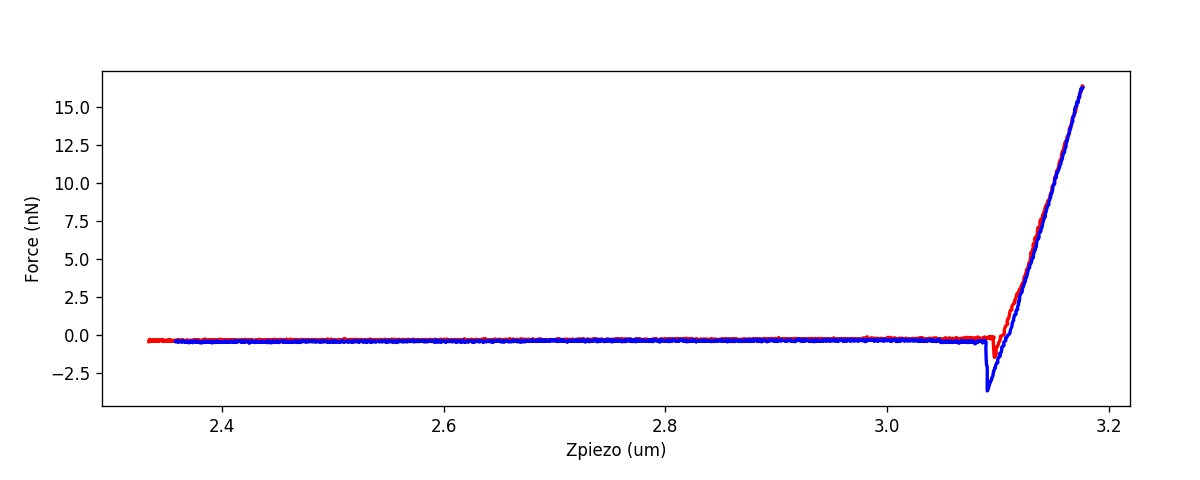
\includegraphics[width=110mm]{chapter4/EgRawGraph.jpg}
\end{center}
\caption{An example of a individual graph produced at this point. Minimal processing has been done with only the deflection converted into force (nN) vs piezo z position ($\mu$m)}
\label{fig:EgRawGraph}                 % Reference label to the figure.
\end{figure}


%Discuss how the 

In order for the script to perform correctly on each of the curves, there needs to be a long enough stretch of data for the approach and a long enough contact region. In the vast majority of cases this is true; there are a few cases where during normal operation an over correction occurs, resulting in the captured range of data to be shifted. For a given curve there are 3 identifiable regions; the approach phase, with no identifiable forces applied on the tip, the interaction phase, where the tip is either repulsed or attracted to the surface, and the contact phase, where the tip is in contact with the surface. These phases are shown in figure \ref{fig:forceAnatomy} as A, B and C respectively. A good curve will include all of these phases in it's snapshot of data, thereby allowing a clear representation of the variable forces applied upon the tip. The operational parameters of the AFM defined by the user are done so in a way to collect the most amount of data (aka setting the snapshot) during acquisition around the transitional point while reducing the amount of unneeded movement towards the surface, and equally reducing the amount of strain forced upon the cantilever during the contact region. At high strains the surface of the cantilever or petri dish can become damaged, or the cantilever can become damaged or break. As the conversion of deflection into force requires the spring constant to remain the same, and damage can cause this conversion to no longer remain true, any damage over the operation is considered by reviewing the curves over time. If there is a significant drift in the shape of the curve over the process of a site, then this is highlighted, and the experiment repeated. In the event of the cantilever breaking the AFM ceases to function and therefore data collection stops. As the retract curve immediately follows the approach curve, the retract curve inherits the same snapshot of data range.%usually followed by ample swearing

%defining the voltage input for the next step based off the previous step.

%Make frame of reference image


%Talk more about binning - find a paper

%How I know a curve is not typical by eye. Example based approach?
%Show example bad graphs

%mfp.comp_def_deriv

\begin{figure}[h!]     %Insert a figure as soon as possible
        \begin{center}
          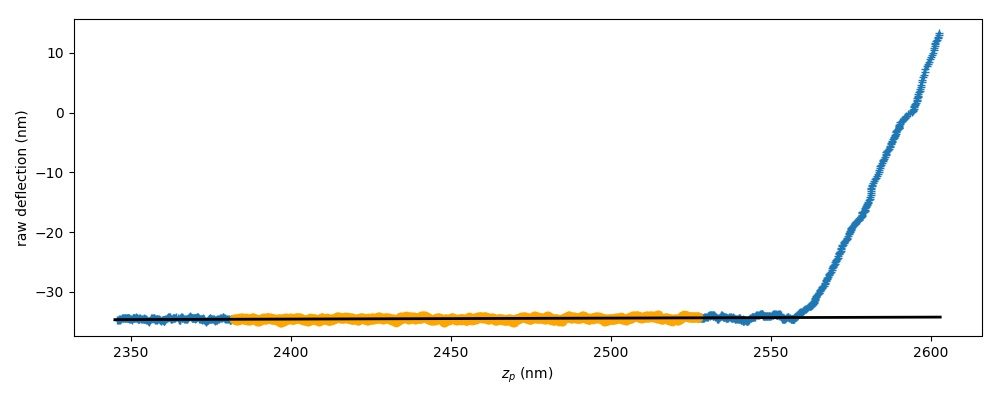
\includegraphics[width=110mm]{chapter4/farfielddrift.jpg}
\end{center}
\caption{An example of a individual graph produced for a single approach curve. The orange region of the graph is the area used in the farfield drift reduction and used to set the floor of the data to 0.}
\label{fig:farfielddrift}                 % Reference label to the figure.
\end{figure}

%proc_force_sep() and comp_def_deriv() (?)
%guess contact point and work backwards, uses np.where
%cthresh = 'first pass' guess deflection threshold for contact. cthresh is set manually
%returns de-drifted zp, df.  data used to de-drift runs from dfit_win:2*dfit_win
%remove_farfield_drift()
Each curve is then processed individually. The first step taken is to address some of the background noise. This is done by taking a linear portion of the curve (see fig \ref{fig:farfielddrift}), where any movement done by the piezo is far enough away that any forces acting between the surface and the cantilever are zero. This removes any farfield drift.  %intending to remove any gradient found along the linear non-contact region. 

This area is defined by a region along this curve, set to use points away from the initial contact area of the curve. Initially the distance traveled per datapoint is calculated by taking the adjusted range of data divided by the total number of datapoints. Based on a combination of user input and backward estimation of the contact area, the data window is carefully aligned along this linear regime. A corresponding graph is then generated to clearly highlight this selected region. This linear horizontal region is then normalised at 0, with the whole dataset translated up or down accordingly.
%Expand upon the contact area user input and estimation
%expand this paragraph

%remove_farfield_drift() end

Afterwards the data is binned into a set of variable sized bins to produce a smoother curve and reduce the effects of noise intrinsic to the system. The size of this set is determined on a case-by-case basis through an iterative process, with a bin size of 5 being most commonly used. In earlier curves where the total number of data points taken was 2000 per curve, the bin size was smaller. Subsequently the size of the data collected was larger which improved the resolution and this enhanced the data analysis. It was determined that increasing the total number of data points to 8000 was optimal. Smoothing the curve in this manner improved the accuracy in which the contact point is defined. A graph was additionally produced with a bin size sweep of $\pm$ 2 to ensure that any features were not lost during binning.
%The size of these bins were based off a paper
%describe binsize better
%Why did I pick the bin sizes that I did
%(basically binning as much data as possible to smooth the curve without losing enough data points)
%Show multiple curves to show the effect of increasing bin size? Yeh bluergh
%How do I know that changing the binsize doesn't change the result or introduce artifacts
%VIVA QUESTION

%After binning, a first degree polynomial is fitted to the selected data. In the case where a suitable fit could not be found for the curve, this set is skipped, and the curve is left untranslated.

%Review this paragraph, expand upon the "estimate produced"
Once binning was complete attention was given to the selection of the data which best represented the area in which the tip has made contact with the surface, i.e. where any piezo movement was translated into cantilever deflection. In general, this selection was defined by reviewing the graphical output from the previous steps. This selection aims to include as much as the graph as possible after the contact point, though it should be highlighted that the deflection is not a purely linear event in practice. In order to ensure that the contact region was estimated reliably, the upper and lower boundaries of the range were sweeped by $\pm$ 5 arbitrary units producing an additional series of curves with this range. This ensured that the final estimated force at contact is within a local parameter minima, i.e. the estimated contact force wasn't independently produced because of a sole artifact, but agreed with the contact forces reported from similar input values.
%Purely linear event - viva question

%Test figure to see if it's readable output in paper
\begin{figure}[h!]    
        \begin{center}
          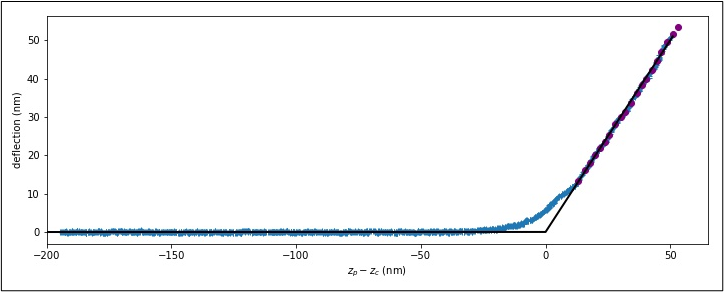
\includegraphics[width=110mm]{chapter4/contactRegion.png}
\end{center}
\caption{An example plot of an approach curve. The area used to help define contact is highlighted by the purple dots overlaying the raw curve.} %word salad
\label{fig:contactRegion}                
\end{figure}

%Put an eqn instead of word salad. Explain intercept better
%Where the extrapolation intercepts the floor line is where we define the contact point
Using this defined region, the data is extrapolated back to the intercept with the horizontal 0 force line. In the case that there is a jump to contact, the jump point is used instead of the interpolated $z_c$. Where the extrapolation intercepts the normalized floor line (i.e. where y = 0) is where $z_c$ is defined. Each curve is then normalised to 0 using z-piezo position ($z_p$) minus z-piezo contact point ($z_p$ - $z_c$) at the point of contact (see fig \ref{fig:contactRegion}). This term is defined as z-separation ($z_\text{sep}$). By defining the contact point as 0 the force at contact can be extrapolated from the curve - by taking the equivalent y-axis value when x is 0.

In some cases, particularly in the measurements made with the JPK NanoWizard AFM (see Section 8.3), intermediate data points through the jump to contact were successfully captured, providing further insights into this phase of the force profile. These data points offer a more detailed understanding of the transition and are discussed in greater depth later in the thesis.

\begin{equation}
z_\text{sep} = z_p - z_c
\end{equation}

%TODO add graph showing a jump to contact calculation

In conceptual terms $z_{sep} \textit{= 0}$ is the point in which the cantilever would come into contact with the surface under no outside stress. In some cases, when a high degree of cantilever movement is applied in the contact phase, the cantilever can bend beyond the the non-linear region of the photodiode detector. This is only present at high deflections, and thus care is taken to ensure that the analysis is done within the linear response region of the photodiode. The non-linear region is where the laser reaches the limits of the photovoltaic cells and the overall signal strength is reduced. Additionally, at higher stresses the cantilever can be subjected to non linear deformation. As the system itself assumes a constant translation from piezo movement during the contact phase into linear deflection recorded by the photodiode, these abnormal data points at the end of the curve are a result of the photodiode's limits. It is in this cases that said recorded can interfere with the processing. as a result, where the behaviour of the curve is inconsistent with the known behaviour of the machine, that said data is removed, though it is important to highlight that said abnormal data only appears after an expected linear contact phase, when the limits of the machine are met. This curve then displayed expected behaviour throughout the approach, interaction and contact phases.

Later in the thesis, particularly in Section 7.5, measurements made with the JPK NanoWizard AFM reveal additional aspects of this part of the force profile, including the "jump to contact" phenomenon. These subsequent findings provide a more nuanced understanding of the force interactions and should be considered alongside the  observations presented here for a more complete picture.
%VIVA QUESTION

After all this processing an averaged curve is is generated by taking all of the individual curves and averaging them together. This is done by progressing along the $z_{sep}$ list, combining their points into a binned point, averaging each bin, then calculating the standard deviation of each bin.

\begin{figure}[h!!!!]    
        \begin{center}
          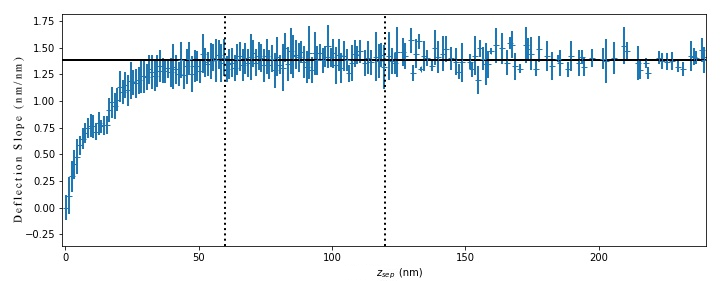
\includegraphics[width=100mm]{chapter4/gradientGraph.png}
\end{center}
\caption{An example plot of the averaged approach gradient. The "approach gradient" in this context refers to the slope of the deflection as the AFM tip approaches the surface. Specifically, it is the rate at which the deflection changes as the AFM piezoelectric element moves the cantilever closer to the sample surface. This gradient provides insight into the force interactions occurring as the tip nears the surface, which is critical for understanding phenomena like the "jump to contact." This graph focuses specifically on the region after contact and the area used to define contact is highlighted by vertical dotted black lines (aka the defined contact region). The horizontal black line indicates the extrapolation of the data. in this case the data is binned to reduce noise. The height of each blue bar indicates the standard deviation for each point.} %units, better y axis
\label{fig:EgAvgDeriv}                
\end{figure}

%Add equation
In order to ensure that the region defined by the operator is correct, a number of diagnostic graphs were produced in order to aid the selection process. The gradient of the deflection is calculated with respect to the stage height in order to highlight the transition between the movement phase and the contact phase of the graph. This is done for individual curves as well as an averaged curve (see \ref{fig:EgAvgDeriv}).

\newpage

These curves are then all plotted on top of one another to check that all curves follow the same rough shape (see fig \ref{fig:proc_force_sep_mastercurve}).

\begin{figure}[h!]     %Insert a figure as soon as possible
        \begin{center}
          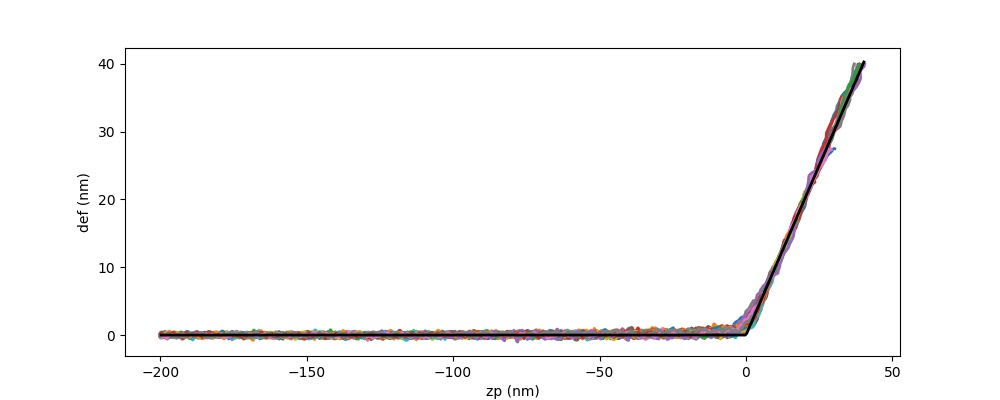
\includegraphics[width=110mm]{chapter4/proc_force_sep_mastercurve.jpg}
\end{center}
\caption{An example plot of all the curves for a given site processed up until this point. A reference black line is overlaid demonstrating what a curve would look like with only terminal electrostatic repulsion. This figure represents about 100 curves aligned atop one another.}
\label{fig:proc_force_sep_mastercurve}                 % Reference label to the figure.
\end{figure}

%histogram of detection slope, not sure if it's worth mentioning, mostly a quick check to see nothing crazy happens

%#mfp.proc_force_sep END

%mfp.plot_force_sep_res 



This resolves in a final averaged and binned force curve (see fig \ref{fig:EgFinalCurve})

\begin{figure}[h!!!]     %Insert a figure as soon as possible
        \begin{center}
          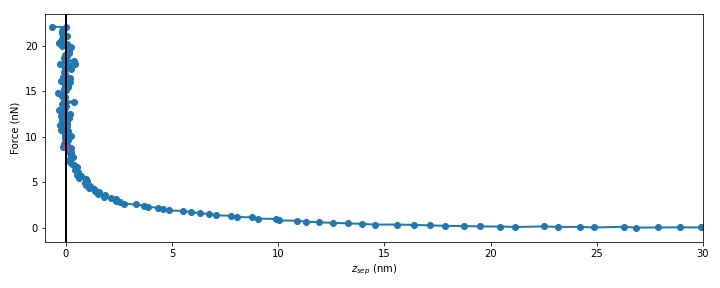
\includegraphics[width=110mm]{chapter4/EgFinalCurve.jpg}
\end{center}
\caption{An example plot of the final processed force curve. The y axis has been translated to show the distance from contact, with a black line highlighting the defined point of contact. The datapoint used to define the force at contact is highlighted in red.}
\label{fig:EgFinalCurve}                 % Reference label to the figure.
\end{figure}

%mfp.get_contact_forces

Afterwards the focus of the script changes to calculating the force applied at contact. Positive forces indicate a repulsive force, negative forces indicate an attractive force. A Savitzky--Golay filter is applied to the data to reduce the noise intrinsic to the data. \cite{SavitzkyGolay} Then the curve is followed algorithmically until it passes over the threshold point - by default, this threshold is defined as the point where the separation between the AFM tip and the surface is 0 nanometers, indicating physical contact.
%VIVA QUESTION

This is done for each individual curve, eventually resulting in a histogram of contact forces (see fig \ref{fig:EgForceHisto}). This provided an insight into the variance between each of the curves, with a wide distribution indicating improper calibration settings for some of the curves. In the cases of outliers, their individual curves were reviewed and used to improve the fitting parameters.

\begin{figure}[h!!!] 
        \begin{center}
          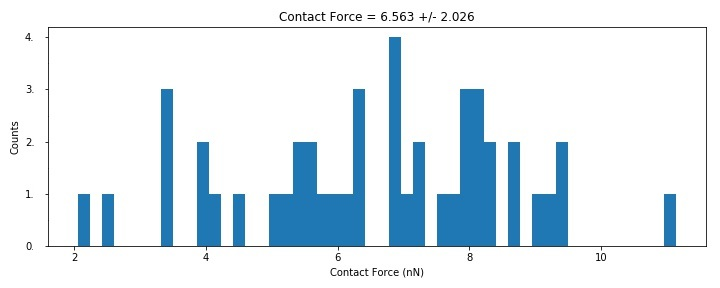
\includegraphics[width=110mm]{chapter4/EgForceHisto.jpg}
\end{center}
\caption{An example of a histogram produced from a set of curves for specific site. The mean force is given at the top with the standard deviation.}
\label{fig:EgForceHisto}              
\end{figure}
%VIVA QUESTION - statsitical properties of distribution

Contact force refers to the force exerted when the AFM tip makes physical contact with the sample surface. This force is measured at the precise moment when the separation between the AFM tip and the surface reaches zero. It can be either repulsive or attractive depending on the nature of the interaction between the tip and the sample. Positive values indicate a repulsive force, often due to surface stiffness or electrostatic repulsion, while negative values signify an attractive force, such as van der Waals forces or adhesion.

In all cases the total number of individual graphs per final force datapoint is between 80-200 curves.

\subsection{Validation of results}

In order to validate that the data produced by the procedure met the precedence set by theory, the Debye length was experimentally determined. This approximation of the Debye length ($\kappa$) was calculated using the equation outlined in chapter 1 (see eqn $1.2$). The experimentally calculated value was then checked against the approximated Debye length across a sweep of concentrations. This was in part to ensure that the procedure gave sensible results as well as a means of detecting invisible sources of contamination.

\begin{figure}[h!!]    
        \begin{center}
          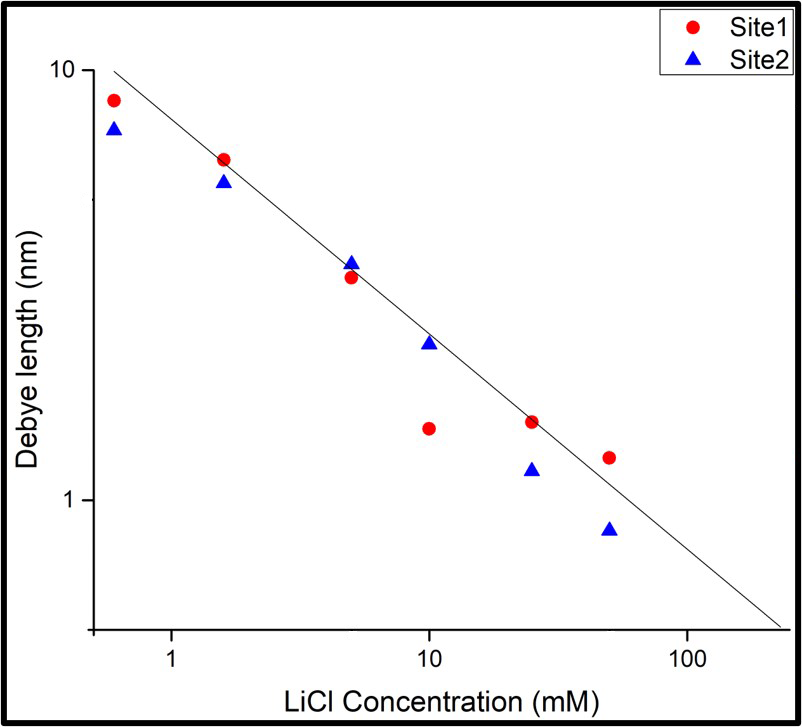
\includegraphics[width=100mm]{chapter4/DebyeLength.png}
\end{center}
\caption{A preliminary graph produced to investigate the expected Debye length vs the recorded Debye length at different salt concentrations. The black line indicates the approximated $\kappa$, whereas site one and two are two different recording areas on the glass surface.}
\label{fig:DebyeLength}                 
\end{figure}

This procedure produced sensible Debye length measurements according to the preliminary data (see fig \ref{fig:DebyeLength}). As a result this procedure was used for subsequent experiments. The Debye length of the interacting silica sphere was calculated by calculating the equation of the curve during the interaction phase and extracting the exponent component (i.e. between the approach and contact phases).
%These curves were used for analysis using the following script mechanics.

%From these results a selection of the concentrations where an observable Debye length was chosen and processed using all of the techniques outlined in this chapter. 
This Debye length measurement procedure indicates strongly that the chosen experimental and processing protocol is appropriate. Additionally the influence of contaminants have been reduced to a minimum from said revised protocol.

\newpage

\section{Nanowizard}

Over the course of the investigation the availability of an alternative AFM became available. When compared to the MFP-1D, the setup is very similar, with one notable exception. This AFM allows for free horizontal control coupled to the AFM head, instead of requiring the operator to disengage each time. Aside from the time saved between changing sites, this allows for techniques such as force mapping to be used (See chapter 2). The setup procedure remained the same as defined before during use with this AFM with any difference being software based, and thus an unnecessary detail for this report. 

\begin{figure}[h!]     
        \begin{center}
          \includegraphics[width=80mm]{chapter4/Nanowizard.png}
\end{center}
\caption{Operation setup for the Nanowizard AFM that was used for force measurements \cite{NWizardPic}.}
\label{fig:Nanowizard.png}                 
\end{figure}

Fortunately the previously established sample preparation and cleaning procedure was adapted with little difficulty with the experimental throughput considerably increased. The tip speed was set to the previously defined speed, \SI{1}{\micro\metre/s} as well as the peak force at 8 nN, unless otherwise stated.

\subsection{Analysis differences for JPK NanoWizard} %What is this an RPG tabletop for scientists?

The output from the Nanowizard was exported from the proprietary JPK file format and refitted to work with the script described above. While the differences in output data structure is dramatic, this was handled by a short reformatting script to translate the data into a usable format. The only differences of note between the two is that the JPK format has fewer significant figures compared to the previous methods.

In the case of force mapping, there are considerably less curves per site. At this point, the previously established curves produced by the MFP-1D for each concentration were used for comparison. Each of the curves is then processed by the script, with a note taken of its x,y $\mu$m offset. Afterwards the averaged contact force (for approach) or adhesive force (for retract) is plotted on a heat map. For each heat map a 10$\times$10 grid was processed, with at minimum 3 curves per site taken, with a \SI{1}{\micro\metre} distance between each site. It should be noted that the software processes an entire grid first, which is to say each site is repeated after all sites of the current grid are done.

\section{Development and Significance of the Force Curve Analysis Software}

The analysis software developed during this research plays a pivotal role in the extraction and interpretation of force curves obtained via Atomic Force Microscopy (AFM). The ability to automatically process large volumes of data with high accuracy and consistency is a key contribution of this thesis, making the software not just a tool, but a significant contribution to the field.

Traditional methods of AFM data analysis often rely on manual interpretation of force curves, which can introduce variability and error due to human judgment. While earlier software tools provided some level of automation, they often lacked the flexibility to handle complex datasets or adapt to the specific needs of different experiments. Equally, the availability of the software is often tied to specific manufacturers and distributors, which limits accessibility. The software developed in this thesis builds on these earlier approaches by offering a more robust, adaptable, and user-friendly platform that can be adapted to any set of results.

This software was designed to address several key challenges. Firstly, by incorporating advanced smoothing techniques, such as the Savitzky-Golay filter, the software effectively reduces intrinsic noise while preserving critical features of the data, such as the 'shelf' observed in certain force profiles. Secondly, the variable-size binning approach allows for more precise control over data smoothing, enabling the detection of subtle force interactions that might be lost in more rigid binning protocols. Finally, the software automates curve fitting to theoretical models, reducing the need for manual intervention and ensuring that the analysis is both consistent and reproducible across different datasets.

One of the significant improvements brought by this software is its robustness against the variability inherent in AFM data. This robustness is particularly evident when comparing the software's performance with older systems that may produce noisier data. The ability to extract meaningful information from such data extends the lifespan of older AFMs, making them viable for current research without the immediate need for expensive upgrades.

The software’s robustness was validated through the analysis in this thesis, given in the following chapters. The consistency of the Debye length calculations across different concentrations, as well as the successful extraction of the 'shelf' feature in noisy data, are testaments to its reliability.

By making this software open source and accessible to the broader scientific community, this thesis not only contributes to the field of AFM but also democratizes access to high-quality data analysis tools. The flexibility of the software allows researchers to adapt it to their specific needs, potentially leading to new discoveries and innovations in surface force studies. It bridges the gap between traditional manual methods and the need for high-throughput, consistent analysis in modern AFM studies.


%TODO: INSERT HEAT MAP HERE LATER AFTER SCRIPT IS DONE BECAUSE AAARGGH

%Show example heatmap

%include any changes observed here. Only difference so far is that it's a faff and that the sig figs is lower on the JPK file format.


%%%Review later:




%%Insert graph showing selection window
%Possibly go into more detail
%Actually do
%Just not right now, your mind can't make sense of it

%Problem solution cycle !!!
%Approach curve analysis
%Process 1/5th curves
%Process new AFM curves
%Write new AFM wrangle code
%Experimental difficulties (DIRT)
%Problem solution cycle
%%%%%%%%%
% TO DO %
%%%%%%%%%
% Expand intro
% Redo graphs from graphing program, expand scope, involve 
% More detail
% Actually describe motivation again
% Rewrite into based off previous chapters


%Don't write too much
%Write what is needed in the text
%The more you write, the higher probability of making mistakes - keep to the point
%Describe results
%Explanation after desc
%Have to be phrases that make sense/say something
%Have a purpose

\chapter{Analysis of Approach Force Curves in Colloidal Systems}
\label{chap:approach_force_curves}

This chapter aims to serve a simple goal. To provide a clear route to extract the force at contact from raw data.  As the raw unprocessed data represents a large volume of data (10,000+ force curves total) the scope of this chapter is kept to one goal, provide the data and justification for the contact forces calculated for each concentration, site and parameter. The results of this analysis is then concluded in Chapter 7, which, is free of the need to justify every data point and thus focuses on the conclusions from this data. 

This data, along with the further analysis provided in chapter 7 is expanded upon, and insights are drawn from this in turn. In order to aid readability/referenceability, this chapter focuses on the data collected during the 

\section{MFP-1D contact force derivation}

For the data collected from the MFP-1D the analytical approach to this elucidation is given in Chapter 4. This section will overview the results for the following LiCl concentrations: 0.6mM, 1.6mM, 5mM, 10mM, 25mM, 50mM, 230mM, 550mM. For each concentration multiple sites are analysed, highlighting features of each curve in preparation for analysis. 

\subsection{A note on rejected curves}

 During the process, several curves were rejected from the data set as part of the processing method, due to the large volume of curves involved in this analysis. This was either due to machine failure to engage in the surface, or due to significant noise due to mechanical failure (over-correction in piezo movement by the AFM or vibrations in the building.) While the initial curves taken on the machine were too noisy, further repeats and refinements to the procedure eventually resulted in usable curves. In some of the data collected, the impact from residual vibrations was mitigated in later datasets by operating the AFM in the night. Other improvements were found by optimising the AFM parameters  - such as tip speed, data collection rate and target force. The optimal parameters found were 0.5Hz for tip speed, setting the data collection rate to maximum and a target force of 8-12 nN. 

\begin{figure}
    \centering
    \includegraphics[width=0.65\linewidth]{chapter5/miss_error.png}
    \caption{A graph demonstrating a rejected curve. In this case the AFM failed to reach the surface for the recorded data, leading to a single up and down motion. In this case red is the approach curve and blue is the retrace curve.}
    \label{fig:miss-error}
\end{figure}

The other reason for rejected curves was due to the shift of the snapshot window providing too little data in either the approach phase or the contact phase (covered in Chapter 4). 

\subsection{Contact force calculations}

In this results section, the contact force graphs displayed represent only a subset of the total analyzed graphs, selected to illustrate the most significant aspects of the analysis procedure. The ones chosen here represent the typical majority of the curves, with outliers not reflected in the dataset. Outliers may be demonstrated, and will be commented on if presented. The remainder of the curves, not shown here, played an instrumental role in guiding the parameter optimization process for the data processing script. This process involved the review and refinement of several hundred thousand curves in order to deal with the noise intrinsic to the system. Ensuring a good fit for these curves is paramount; otherwise, one risks obtaining erratic and misleading graphs that could compromise the integrity of the data interpretation. The selection process for the resulting curves involved the exclusion of certain outliers and repeat measurements, a necessary step taken to refine the data and enhance the clarity of the observed trends. Three types of graphs were chosen for their analysis of the fitting parameters and results: the histogram of contact forces provides a statistical view of the interaction forces at the point of contact, demonstrating the range of forces across the graph. The log-linear plot of the force as a function of the Z-piezo position (in nanometers), highlighting of the separation distance between the AFM tip and the sample surface during the interaction phase. At the top of the graph the transition to the contact phase can be seen. This point of transition is the contact force. The logarithmic scale for force highlights the sensitivity of the AFM in detecting forces at the nanoscale. Finally the overall approach force curve derived from binned data presents a view of the resulting averaged force curve behavior during the approach phase. Each graph was selected for its ability to support the chosen parameters and thus the resulting contact force.

\subsection{Diversity and Range of Data Points}
Each site and corresponding graph included in Chapter 5 were selected to represent the wide range of experimental conditions explored in this study. The diversity of salt concentrations (ranging from 0.6mM to 550mM) provides a comprehensive view of how the interactions between colloidal particles change under different ionic strengths. By including data from various sites, the results shown are not biased by localized effects, but are reflective of the overall behavior of the system. This approach highlights trends across the dataset, such as the transition from repulsive to attractive forces as the salt concentration increases, which is required for understanding the underlying mechanisms governing colloidal stability.

The "shelf" feature observed in some of the following force profiles is of particular interest because it indicates a potential secondary interaction mechanism that might not be explained by traditional DLVO theory alone. The inclusion of these specific sites and graphs where the shelf feature is prominent was intentional. Highlighting this phenomenon is important because it may suggest the presence of complex surface interactions, possibly related to surface roughness or heterogeneities, which could have significant implications for the interpretation of force measurements in colloidal systems.

The presence of the shelf at different concentrations and its persistence across various sites suggest that it is not a random artifact but a consistent phenomenon that warrants deeper analysis. Including these graphs provides a more complete picture of the force interactions at play and challenges us to consider additional factors that may influence colloidal stability beyond those traditionally considered in DLVO theory. A dedicated analysis of this observation is provided later in section 8.3. This shelf feature isn't without literature precedent however, as it has been observed previously. \cite{Kilpatrick2013DirectlyProbing} \cite{guleryuz2012afm}

%0.6mM
\insertapproachfigures{5}{0.6}{1}{Site one demonstrates one of the difficulties with collecting the data at the lower ranges of the molar concentrations. As the repulsive force is over a wider range there is a smaller window captured of the contact phase. This means that when trying to fit to the curve, there is less data available to provide a solid fit.  As such, a slight bowing effect is seen in the binned average curve.
Additionally, the signal to noise ratio in this curve is significantly high compared to others, with the later graphs of higher concentrations generally having a better signal to noise ratio.

38 curves in total were processed. Of these processed curves the average contact force was 5.2 nN $\pm$ 1.5 nN.}
\insertapproachfigures{5}{0.6}{2}{Site two demonstrates the lowest observed force for this concentration, highlighting a high degree of variability between sites. However, this may be due to difficulty in finding a good fit. As the maximum contact force was capped, some of the curves ended within the contact region, or just after, limiting the number of viable curves.

13 curves in total were processed.  Of these processed curves the average contact force was 3.6 nN $\pm$ 0.3 nN.}
\insertapproachfigures{5}{0.6}{3}{Site three demonstrates an ideally fitted curve, however in the log-linear plot an irregularity is seen - the point in which the contact force area is raised up the graph. This is due to the large amount of noise seen during this interface phase, giving a large variation in the contact force histogram.

29 curves in total were processed. Of these processed curves the average contact force was 4.7 nN $\pm$ 1.4 nN.}
% ... and so on for other sites and concentrations.

%1.6
\insertapproachfigures{5}{1.6}{1}{Site one represents an good example of a typical well-behaved curve, where the processing is able to extract out a clear signal from the noise, and thus a clearly distributed contact force.

140 curves in total were processed. Of these processed curves the average contact force was 2.6 nN $\pm$ 0.6 nN}
\insertapproachfigures{5}{1.6}{2}{Site 2 demonstrates an interesting feature - a region where there seems to be two contact phases. As DLVO doesn't explain any dual barrier features this is rather unexpected. One explanation may be that as the two surfaces approach one another some aspect (for example a small topographical protrusion or a small aggregate of ions) prevents full contact between the sphere and surface, which then slips or is overcome, allowing full contact later. It is important to note that this feature is present throughout the dataset, and survived the binning and averaging process, and thus is a consistent feature in this site.

113 curves in total were processed. Of these processed curves the average contact force was 4.5 nN $\pm$ 0.5 nN}

%5
\insertapproachfigures{5}{5}{1}{Site one demonstrates a similar, but weaker feature seen in 1.6 mM site 2 observable in the log-lin plot. The overall binned fit demonstrates a suitable fit, so it remains to be a feature of this site. Equally, this site demonstrates the weakest repulsive force in the set.

128 curves in total were processed. Of these processed curves the average contact force was 2.2 nN $\pm$ 0.5 nN}
\insertapproachfigures{5}{5}{2}{Site two demonstrates the same feature, but slightly less prominent again.

110 curves in total were processed. Of these processed curves the average contact force was 3.1 nN $\pm$ 0.7 nN}
\insertapproachfigures{5}{5}{3}{Site three once again has the feature seen across all of the force curves at this concentration

114 curves in total were processed. Of these processed curves the average contact force was 3.8 nN $\pm$ 0.5 nN}

1.6 mM site 2 and 5 mM presents an interesting and repeatable shelf seen in the force profiles across all different sites. There are a number of theories as to what this feature may be. For one If the AFM tip encounters a region of the sample with a topological feature that does not mesh well with the surface it could provide the observed barrier. This feature can then hold the tip back from fully sliding down until a threshhold force determined by the surface roughness is presented. Once this threshold force is overcome it then "slips" down further into contact.

%10 2 sites
\insertapproachfigures{5}{10}{1}{Site 1 demonstrates a noisy top of the graph, which can sometimes happen when the AFM oversteers and provides too much force onto the sample.

130 curves in total were processed. Of these processed curves the average contact force was 1.8 nN $\pm$ 1.1 nN}
\insertapproachfigures{5}{10}{2}{119 curves in total were processed. Of these processed curves the average contact force was 3.8 nN $\pm$ 0.4 nN}
\insertapproachfigures{5}{10}{3}{124 curves in total were processed. Of these processed curves the average contact force was 4.4 nN $\pm$ 0.5 nN}

%25 3 sites
\insertapproachfigures{5}{25}{1}{Site 1 demonstrates a high degree of noise in the binned average curve and demonstrates towards what curves could be without the involved processing

144 curves in total were processed. Of these processed curves the average contact force was 2.2 nN $\pm$ 1.7 nN}
\insertapproachfigures{5}{25}{2}{Site 2 also demonstrates a shelf feature.

124 curves in total were processed. Of these processed curves the average contact force was 2.7 nN $\pm$ 1.1 nN}
\insertapproachfigures{5}{25}{3}{76 curves in total were processed. Of these processed curves the average contact force was 3.9 nN $\pm$ 1.5 nN}

%50 2 sites
\insertapproachfigures{5}{50}{1}{50mM both demonstrates the presence of the shelf feature, as well the contact force following the trend of decreasing over time.

104 curves in total were processed. Of these processed curves the average contact force was 3.3 nN $\pm$ 0.6 nN}
\insertapproachfigures{5}{50}{2}{105 curves in total were processed. Of these processed curves the average contact force was 2.8 nN $\pm$ 0.7 nN}

%230 2 sites
\insertapproachfigures{5}{230}{1}{230mM demonstrates the point in which the repulsive force observed is close to 0. The shelf feature observed in the 230mM data is particularly significant because it suggests a region of weak attraction following the initial contact. This feature is not consistently observed in all graphs, which could be due to variations in local surface roughness, heterogeneity in the colloidal particles, or slight differences in the approach speed of the AFM tip.

109 curves in total were processed. Of these processed curves the average contact force was 2.2 nN $\pm$ 0.3 nN}
\insertapproachfigures{5}{230}{2}{84 curves in total were processed. Of these processed curves the average contact force was 0.8 nN $\pm$ 0.4 nN}

%550 3 sites
\insertsnowflakefigures{5}{550}{1}{500mM marks the situation where the charge screen starts to overcome the electrostatic repulsion, giving way to an attractive force instead. Interestingly the shelf effect is still observed despite the attractive nature of the two surfaces.

84 curves in total were processed. Of these processed curves the average contact force was -0.3 nN $\pm$ 0.1 nN}
\insertsnowflakefigures{5}{550}{2}{107 curves in total were processed. Of these processed curves the average contact force was -0.1 nN $\pm$ 0.1 nN}
\insertsnowflakefigures{5}{550}{3}{89 curves in total were processed. Of these processed curves the average contact force was -0.1 nN $\pm$ 0.1 nN}

\section{Overall force vs LiCl concentration graph}

The forces calculated at the point of contact were subsequently plotted on a graph. For the values, the average was taken, the standard deviation was calculated by:

\begin{equation}
Stdev_{avg} = \sqrt{\frac{{x_1}^2 + {x_2}^2 + {x_3}^2}{n_{num}}}  
\label{eq:Stdevavg}
\end{equation}

Where $x$ is the site's standard deviation and $n_{num}$ is the number of sites in the calculation (i.e. where there were 3 sites, this value was 3).

 In the case of a LiCl concentration of 550 mM, the attractive force was utilized in the plot due to the alteration in the nature of the force curve.

\begin{figure}
    \centering
    \includegraphics[width=1\linewidth]{chapter5/Average Approach.png}
    \caption{All sites' calculated force at contact with standard deviation error bars. There is an observed trend of increasing LiCl concentration leading to a decrease in repulsive force, until the repulsive force becomes attractive.}
    \label{fig:site1cont}
\end{figure}

The overall graph demonstrate the force at contact appears to decrease with increasing LiCl concentration. The reality for each of the sites is that they were exposed to different tips and different sites. As the AFM used was unable to save site locations, site 1, 2 and 3 aren't the same spacial location on the glass between salt concentrations.

An interesting observation however is in the error bars and thus the variability or uncertainty of the measurements. Larger error bars at middling concentrations, especially noticeable at 25mM, might suggest greater variability in the interaction forces measured at these points.

The dotted line was added to guide the rough direction of the plots, which indicates that as salt concentration increases, the force requires for silica particles to come into contact decreases, eventually giving way to an attraction between the particles. This is likely due to the higher salt concentrations screening the electrostatic interactions. However, another interesting aspect is an observed plataeu between 5 - 50mM ionic strengths, potentially indicating a critical ion concentration needed to disrupt the electrostatic repulsion enough in this region.

These calculated forces are then expanded upon in chapter 7, with further analysis into potential reasons as to why these trends are observed.

\section{Discussion of Force Measurements and Salt Concentration Effects}

The interaction forces between silica surfaces in electrolyte solutions have been a significant area of study in surface science, particularly in understanding the influence of varying salt concentrations on adhesion forces. The results obtained in this thesis, particularly regarding the influence of LiCl concentration on the contact forces between silica particles, align with and extend findings from previous studies such as those by Guleryuz et al. (2012) and Kostakis et al. (2006). \cite{Kostakis2006} \cite{Guleryuz2012}

Guleryuz et al. (2012) performed AFM measurements of forces between silica surfaces in the presence of NaCl and reported that increasing the salt concentration significantly reduces the electrostatic repulsion between the surfaces. This reduction in repulsion allowed for a more pronounced adhesion force as the surfaces approached closer under the influence of the van der Waals attraction. Specifically, their study showed that at higher pH levels, where the silica surface is more negatively charged, the presence of high NaCl concentrations reduced the Debye length, thereby diminishing the range of the electrostatic double-layer repulsion and resulting in a higher adhesion force. In the context of the findings presented in this Chapter, a similar trend was observed, with LiCl instead, where increasing concentrations led to a decrease in the repulsive forces and a corresponding increase in the adhesion forces measured between the silica particles. \cite{Guleryuz2012}

The work by Kostakis et al. (2006) further complements these findings by exploring the stabilization of bubbles by silica particles in high salt concentrations. They noted that at high NaCl concentrations, the surface structures, such as polysilic acid chains, collapsed, leading to a significant reduction in steric repulsion and an increase in adhesion. This observation parallels the results of Chapter 5, as it suggests that the reduced repulsive force, and thus increased contact forces observed at higher LiCl concentrations could be due to a similar collapse of surface structures on the silica particles, thereby allowing closer surface contact and stronger adhesion.  \cite{Kostakis2006} 

The similarities in the behavior of silica surfaces in NaCl and LiCl solutions across these studies reinforce the hypothesis that the ionic strength of the solution plays a crucial role in modulating the balance between repulsive and attractive forces in colloidal systems. The increased adhesion forces observed in the presence of high salt concentrations, as reported by Guleryuz et al. and Kostakis et al., provide a valuable comparison point for the results discussed in this thesis. This comparison highlights the generality of the observed phenomena across different electrolytes, confirming that the reduction in electrostatic and steric repulsion with increasing ionic strength is a robust effect influencing contact forces in AFM measurements.

It emphasizes the importance of considering both the chemical nature of the electrolyte and the pH of the solution when analyzing AFM force profiles, which is one aspect that is expanded upon in Chapter 7. The observed increase in adhesion force with higher LiCl (salt) concentrations is consistent with the broader body of literature, and leads us into our next chapter, which focuses on the adhesive nature of the silica tip to the borosilica surface.




%Retract curve analysis
%Process 4/5th curves
%New AFM wrangling
%CHAPT 6
\chapter{Retract force curves}

\section{Introduction}

\subsubsection{Analysis of Silica-silica retract curves}

Further analysis is currently being performed on the retract curves utilizing an adapted version of the approach script. This is done in a similar method to the previous, with parameters refined by eye, then the range tested by adding or subtracting 10nm to the contact fitting region. The literature surrounding silica-silica force curves taken in salt usually omit the retract curves, while only a few mention them \cite{Retrace}. 

\cite{John}.

\newpage

\subsection{0.6mM}
%This is saved locally
\newpage.
\newpage

\subsection{1.6mM}
.
\newpage.
\newpage

\subsection{5mM}
.
\newpage.
\newpage

\subsection{10mM}

\newpage

\subsection{25mM}

\newpage

\subsection{50mM}

\newpage

\subsection{230mM}
.
\newpage.
\newpage

\subsection{550mM}
.
\newpage.
\newpage

\section{Effects of hydrodynamics}
.
\newpage.
\newpage

\section{Dwell time effects}
.
\newpage.
\newpage.
\newpage

\section{pH effects}
.
\newpage.
\newpage

\section{Force mapping}

\chapter{Force event analysis and conclusions}
\newpage

%Bad graphs
%Thesis correction post viva
%Priority based management of time
%Computed the time I have left

%Bacterial
%\chapter{Bacterial colloids AFM}

\section{Introduction}

In addition to this in liquid force curves were produced from probing bacteria. The possibility of force mapping a bacterial surface was investigated, but ultimately ruled impossible on the current machine. However efforts have been made to procure access to a more suitable AFM (See section 2.1).

\subsection{AFM tip treatment} %Is this worth mentioning?

Successful adaption and development of the glass treatment to AFM tips was performed. In particular a tip was treated with DCDMS surface coating. This tip was planned to be used with force mapping to investigate the presence of adhesive patches theorized by the group \cite{Teun1} and other literature \cite{Patchy}. 

\subsection{Attaching bacteria to a cantilever}
\newpage

\section{Bacterial force curves}

\newpage
\newpage
\newpage

\chapter{Conclusion}



\backmatter

\singlespace

\phantomsection
\addcontentsline{toc}{chapter}{\bibname}
% Choose a bibliography style to suit your taste here
% This one was downloaded from http://web.reed.edu/cis/help/latex/bibtexstyles.html (June 2012)
\bibliographystyle{ChicagoReedweb}
%\bibliography{chapter2/chapter2bib}
\bibliography{chapter1/chapter1bib,chapter2/chapter2bib,chapter3/chapter3bib,chapter4/chapter4bib,chapter5/chapter5bib}

\end{document}
